%!TEX TS-program = xelatex
%!TEX encoding = UTF-8 Unicode

\documentclass[a4paper,11pt,twoside]{book}
\usepackage{upatras-thesis}


%
% These commands need to be defined in order to produce a correct and personalized document
%
\newcommand{\shortdoctitle}{Διπλωματική Εργασία}
\newcommand{\doctitle}{Επεξεργασία \& Απεικόνιση Μεγάλου Όγκου Οικονομικών Δεδομένων}
\newcommand{\docsubtitle}{}
\newcommand{\division}{Ηλεκτρονικής \& Υπολογιστών}
\newcommand{\lab}{Ενσύρματης Τηλεπικοινωνίας}

\newcommand{\me}{Γεωργίου Λυδάκη}
\newcommand{\studnum}{227547}
\newcommand{\keywords}{forex, data visualization, recommendation systems}
\newcommand{\monthyear}{Σεπτέμβριος 2016}

\newcommand{\supname}{Κωνσταντίνος Μουστάκας}
\newcommand{\suptitle}{Επίκουρος Καθηγητής}
\newcommand{\headofdivision}{Νικόλαος Φακωτάκης}
\newcommand{\headofdivisiontitle}{Καθηγητής}

\author{\me}


% PDF settings
%
\hypersetup
{
    pdfauthor={\me},
    pdftitle={\shortdoctitle},
    pdfsubject={\doctitle},
    pdfkeywords={\keywords}
}

\begin{document}


\pagenumbering{roman}
%set the number of sectioning levels that get number and appear in the contents
\setcounter{page}{3}

\begin{titlepage}
\begin{center}
% Upper part of the page
\textsc{\textbf{\large ΠΑΝΕΠΙΣΤΗΜΙΟ ΠΑΤΡΩΝ - ΠΟΛΥΤΕΧΝΙΚΗ ΣΧΟΛΗ}\\
\large ΤΜΗΜΑ ΗΛΕΚΤΡΟΛΟΓΩΝ ΜΗΧΑΝΙΚΩΝ\\ΚΑΙ ΤΕΧΝΟΛΟΓΙΑΣ ΥΠΟΛΟΓΙΣΤΩΝ}\\[0.5cm]


\includegraphics[width= 5cm]{up_stamp}\\[0.5cm]  

\textsc{\Large τομέας: \division \\
εργαστήριο: \lab }\\[1cm]

\textsc{\uline{\LARGE{\shortdoctitle }}}\\ [0.5cm]
του φοιτητή του Τμήματος Ηλεκτρολόγων Μηχανικών και Τεχνολογίας\\
Υπολογιστών της Πολυτεχνικής Σχολής  του Πανεπιστημίου Πατρών\\[1cm]

\textsc{\LARGE \me }\\[0.5cm]
\textsc{\Large αριθμός μητρώου: \studnum}\\[1cm]

\uline{\large Θέμα}\\[0.5cm]
\textbf{\large \doctitle }\\[1cm]
\uline{\large Επιβλέπων}\\[0.5cm]
\large \suptitle \, \supname \\[1cm]
\large{Αριθμός Διπλωματικής Εργασίας: }\hspace{3cm}
\vfill
% Bottom of the page
\large{Πάτρα, \monthyear}
\end{center}
\end{titlepage}

\clearemptydoublepage

\pagestyle{empty}
\begin{center}
{\LARGE ΠΙΣΤΟΠΟΙΗΣΗ\\[1cm]}
\large Πιστοποιείται ότι η διπλωματική εργασία με θέμα\\[1cm]
\textbf{\large \doctitle }\\[1cm]
του φοιτητή του Τμήματος Ηλεκτρολόγων Μηχανικών και Τεχνολογίας Υπολογιστών\\[1.5cm]
\me \\[0.5cm]
(Α.Μ.: \studnum )\\[1.5cm]
παρουσιάτηκε δημόσια και εξετάστηκε στο τμήμα  Ηλεκτρολόγων Μηχανικών και Τεχνολογίας Υπολογιστών στις\\[1cm]
\Large{\_\_/\_\_/\_\_\_}\\[1.5cm]
\end{center}
\begin{minipage}{0.5\textwidth}
\begin{flushleft} \large
Ο Επιβλέπων\\[4cm]
\supname \\
\emph{\suptitle}
\end{flushleft}
\end{minipage}
\begin{minipage}{0.5\textwidth}
\begin{flushright} \large
Ο Διευθυντής του Τομέα\\[4cm]
\headofdivision\\
\emph{\headofdivisiontitle}
\end{flushright}
\end{minipage}

\clearemptydoublepage

\pagestyle{empty}
\begin{center}
\Large{Στοιχεία διπλωματικής εργασίας}\\[1cm]
{\large Θέμα:}
\textbf{\large \doctitle}\\[1cm]
\large {Φοιτητής: \textbf{\me}\\[1cm]
\large{Ομάδα επίβλεψης}\\
\textbf{\suptitle \, \supname}\\
\textbf{Βαθμίδα και Ονοματεπώνυμο Συνεπιβλέποντα}\\
\textbf{Ονοματεπώνυμο Διδακτορικού Φοιτητή}\\[1cm]
Εργαστήρια\\
\lab \\[1cm]
Περίοδος εκπόνησης της εργασίας:\\ Μήνας Έτος - Μήνας Έτος\\[1cm]
Η εργασία αυτή γράφτηκε στο \XeLaTeX{} και χρησιμοποιήθηκε η γραμματοσειρά GFS Didot του Greek Font Society.}
\end{center}

\clearemptydoublepage

\pagestyle{plain}
\begin{center}
{\LARGE Περίληψη}\\[1cm]
\end{center}

\lettrine[findent=2pt]{\fbox{\textbf{H}}}{ } δημιουργία ενός Συστήματος Συστάσεων (Recommender System – RS) απαιτεί καλή γνώση του αντικειμένου το οποίο αφορά ο recommender. Γι’ αυτό είναι σημαντικό ένας μηχανικός να μπορεί να δημιουργήσει γρήγορα «διαισθήσεις» πάνω στα δεδομένα στα οποία δουλεύει. Η χρήση απεικονίσεων κατά τη διάρκεια του σχεδιασμού και υλοποίησης του RS μπορεί να βοηθήσει σε μεγάλο βαθμό την εξοικείωση του μηχανικού με τα δεδομένα και το πεδίο στο οποίο δουλεύει. Συγκεκριμένα, σ’ αυτή τη διπλωματική ασχοληθήκαμε με απεικονίσεις που σκοπεύουν να βοηθήσουν τον μηχανικό στη διαδικασία επιλογής χαρακτηριστικών για τον υπολογισμό ψευδο-αξιολογήσεων (pseudo-ratings) για ένα Σύστημα Συστάσεων Συνεργατικού Φιλτραρίσματος με Έμμεσες Αξιολογήσεις (Collaborative Filtering with Implicit Feedback). 

\clearemptydoublepage

\begin{center}
{\LARGE Ευχαριστίες}\\[1cm]
\end{center}

\lettrine[findent=2pt]{\fbox{\textbf{Ό}}}{σο} κι αν φαίνεται σαν ατομική δουλειά η παρούσα εργασία, στην πραγματικότητα βοήθησαν αρκετοί άνθρωποι (ο καθένας με το δικό του τρόπο) για να ολοκληρωθεί. 

\clearemptydoublepage

\pagestyle{fancy}

\tableofcontents
%\mainmatter % book mode only
\clearemptydoublepage

\pagenumbering{arabic}
\setcounter{page}{1}

%!TEX root = ../main.tex

\chapter*{Εισαγωγή}
\markboth{Εισαγωγη}{}
%\vspace{-1.3in}
\lettrine[findent=2pt]{\fbox{\textbf{Η}}}{} δημιουργία ενός Συστήματος Συστάσεων (Recommender System – RS) απαιτεί καλή γνώση του αντικειμένου το οποίο αφορά ο recommender. Γι’ αυτό είναι σημαντικό ένας μηχανικός να μπορεί να δημιουργήσει γρήγορα «διαισθήσεις» πάνω στα δεδομένα στα οποία δουλεύει. Η χρήση απεικονίσεων κατά τη διάρκεια του σχεδιασμού και υλοποίησης του RS μπορεί να βοηθήσει σε μεγάλο βαθμό την εξοικείωση του μηχανικού με τα δεδομένα και το πεδίο στο οποίο δουλεύει. Συγκεκριμένα, σ’ αυτή τη διπλωματική ασχοληθήκαμε με απεικονίσεις που σκοπεύουν να βοηθήσουν τον μηχανικό στη διαδικασία επιλογής χαρακτηριστικών για τον υπολογισμό ψευδο-αξιολογήσεων (pseudo-ratings) για ένα Σύστημα Συστάσεων Συνεργατικού Φιλτραρίσματος με Έμμεσες Αξιολογήσεις (Collaborative Filtering with Implicit Feedback). 

\clearemptydoublepage

\chapter{Χρηματηριστηριακές Συναλλαγές \& Συναλλάγμα}\label{ch:chap1}
%!TEX root = ../main.tex



\section{Εισαγωγή στις Χηματιστηριακές Συναλλαγές}

\lettrine[findent=2pt]{\fbox{\textbf{Ο}}}{ι} χρηματιστηριακές συναλλαγές (trading) είναι ένας ενεργός τρόπος συμμετοχής στις χρηματοπιστωτικές αγορές. Αντί να αναζητούν κέρδη από μακροπρόθεσμες ανοδικές τάσεις στις αγορές, οι χρηματιστές ψάχνουν για βραχυπρόσθεσμες κινήσεις των τιμών έτσι ώστε να επωφελούνται και από τις ανοδικές αλλά και από τις καθοδικές κινήσεις των αγορών.


\clearemptydoublepage

\chapter{Απεικόνιση Δεδομένων}\label{ch:chap2}
%!TEX root = ../main.tex



\section{Τι είναι η Απεικόνιση Δεδομένων}

\lettrine[findent=2pt]{\fbox{\textbf{Κ}}}{ατά} την αποτύπωση οποιουδήποτε αναλογικού σήματος $S(t)$ σε ψηφιακή μορφή $S_i$, πραγματοποιείται μια διαδικασία που ονομάζεται \emph{δειγματοληψία (sampling)} κατά την οποία ένα συνεχές σήμα γίνεται διακριτό και στη συνέχεια εφαρμόζουμε \emph{κβαντισμό} στις τιμές του, για να περάσουμε σε ψηφιακή αναπαράσταση. Όπως φαίνεται και στο σχήμα \ref{fig:sampling}, σε διακριτές χρονικές στιγμές λαμβάνουμε την τιμή του αναλογικού σήματος (μέσω ενός μετατροπέα Αναλογικού σε Ψηφιακό (ADC)) κι έτσι δημιουργούμε μια σειρά από τιμές (\emph{δείγματα}) τα οποία έχουν συγκεκριμένη και σταθερή χρονική απόσταση $T_s$. Η χρονική απόσταση έχει νόημα μόνο ως προς το αναλογικό σήμα, ενώ στην ψηφιακή μορφή των δειγμάτων αναφερόμαστε σε αυτά με ένα δείκτη $n$ και μεταξύ αναλογικού και ψηφιακού σήματος ισχύει ότι $S_i=S(nT_s)$.
\begin{figure}[h]
  \centering
  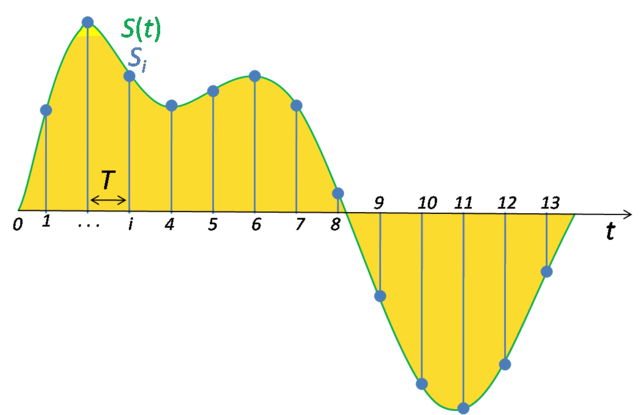
\includegraphics[width=0.6\textwidth]{Signal_Sampling}
  \caption{Δειγματοληψία ενός αναλογικού σήματος}
  \label{fig:sampling}
\end{figure}
Κατά τη δειγματοληψία ``χάνουμε'' αρκετή από την πληροφορία που περιέχει το αναλογικό σήμα, καθώς οι τιμές που βρίσκονται μεταξύ των διαστημάτων $T_s$ όπου λαμβάνουμε δείγματα δε λαμβάνονται υπόψη. Ακόμη, λόγω της πεπερασμένης ακρίβειας των ψηφιακών συστημάτων για αναπαράσταση αριθμών, η τιμή που έχει το σήμα στρογγυλοποιείται στην πλησιέστερη (είτε μεγαλύτερη είτε μικρότερη) τιμή που μπορεί να αναπαραστήσει το σύστημά μας.

Όπως γίνεται αντιληπτό, σε πολλές των περιπτώσεων η δειγματοληψία μπορεί να έχει καταστροφικές συνέπειες για το αναλογικό σήμα. Ωστόσο, υπό προϋποθέσεις, μπορεί να είναι αντιστρεπτή διαδικασία -- μπορούμε δηλαδή από τα δείγματα που έχουμε λάβει να επιστρέψουμε στην αναλογική μορφή του σήματος. Οι προϋποθέσεις αυτές ορίζονται από το θεώρημα \emph{Shannon-Nyquist} (\ref{thrm:shannon-nyquist}), ως:
\\
\begin{theorem}[Shannon-Nyquist]
	\label{thrm:shannon-nyquist}
	Ένα σήμα με μέγιστη συχνότητα $f_{max}$ μπορεί να ανακτηθεί από τα δείγματά του, αν αυτά ληφθούν με συχνότητα $f_s>2f_{max}$, ή αλλιώς με περίοδο $T_s<\frac{1}{2f_{max}}$. \cite{proakis_sampling}
\end{theorem}
\clearemptydoublepage

\chapter{Συστήματα Συστάσεων}\label{ch:chap3}
%!TEX root = ../main.tex



\section{Εισαγωγή στα Συστήματα Συστάσεων}

\lettrine[findent=2pt]{\fbox{\textbf{Σ}}}{ε} πολλά πεδία, καταναλωτές παρουσιάζονται με μια πληθώρα επιλογών και καλούνται να λάβουν κάποια απόφαση. Αυτή μπορεί να είναι ποια ταινία να δουν στο Netflix, ποιο βιβλίο να αγοράσουν από το Amazon, ή στην περίπτωσή μας ποιο ζεύγος συναλλάγματος να παίξουν σε μια πλατφόρμα Forex Trading. Τα Συστήματα Συστάσεων έρχονται να βοηθήσουν τους χρήστες τους δίνοντας συστάσεις βάση διαφόρων παραγόντων, όπως τα προηγούμενα ζεύγη που έπαιξαν, το ιστορικό αγορών τους ή τις αξιολογήσεις ταινιών που έχουν κάνει. 

\section{Τύποι Συστημάτων Συστάσεων}

\lettrine[findent=2pt]{\fbox{\textbf{Τ}}}{α} Συστήματα Συστάσεων μπορούν να χωριστούν σε δύο κατηγορίες ανάλογα με τη προσέγγιση που ακολουθούν· τα Βασισμένα σε Περιεχόμενο (Content Based) και τα Συνεργατικού Φιλτραρίσματος (Collaborative Filtering). Τα πρώτα σκοπεύουν στη δημιουργία ενός προφίλ για κάθε χρήστη ή κάθε προϊόν τα οποία χρησιμοποιούνται για να βρεθούν σχέσεις μεταξύ των χρηστών και προϊόντων. Τα προφίλ μπορούν να περιέχουν στατιστικά ή απαντήσεις από σχετικά ερωτηματολόγια και γενικότερα εξωτερικές πληροφορίες, που μερικές φορές είναι δύσκολο να συγκεντρωθούν. Ένα γνωστό Content Based σύστημα είναι το Music Genome Project, που χρησιμοποιείται από την υπηρεσία ιντερνετικού ραδιοφώνου Pandora.

Από την άλλη πλευρά τα συστήματα Συνεργατικού Φιλτραρίσματος (CF) βασίζονται μόνο σε προηγούμενες συναλλαγές ή αξιολογήσεις, αναλύοντας σχέσεις μεταξύ χρηστών και προϊόντων. Το μεγάλο πλεονέκτημα αυτών των συστημάτων είναι ότι είναι ανεξάρτητα του πεδίου που εφαρμόζονται αλλά παρόλα αυτά είναι ικανά μοντελοποιήσουν πλευρές των δεδομένων που είναι δύσκολο να φανούν χρησιμοποιώντας Content Based συστήματα. Ενώ γενικά τα CF συστήματα είναι πιο αποδοτικά, πάσχουν από το πρόβλημα της «κρύας εκκίνησης» (cold start), δε μπορούν με άλλα λόγια να ανταποκριθούν άμεσα σε νέους χρήστες ή νέα προϊόντα—χρειάζεται το σύστημα να εκπαιδευτεί ξανά στα νέα δεδομένα. Στη διπλωματική χρησιμοποιήθηκε τέτοιου τύπο RS.

Υπάρχουν δύο βασικές υλοποιήσεις Συνεργατικού Φιλτραρίσματος. Οι μέθοδοι γειτνίασης (neighborhood models) και τα μοντέλα λανθανουσών παραγόντων (latent factor models). Τα πρώτα εστιάζουν στο υπολογισμό των σχέσεων μεταξύ προϊόντων ή μεταξύ χρηστών. Η προσέγγιση βασισμένη στα προϊόντα δίνει την προτίμηση ενός χρήστη βάση αξιολογήσεων «γειτονικών» προϊόντων του ίδιου χρήστη. Γειτονικά προϊόντα είναι αυτά που τείνουν να παίρνουν παρόμοιες αξιολογήσεις όταν αξιολογούνται από τον ίδιο χρήστη. Ενώ αντίστοιχα η προσέγγιση βασισμένη στους χρήστες χρησιμοποιεί τις σχέσεις γειτνίασης μεταξύ των χρηστών. 

Από την άλλη τα μοντέλα λανθανουσών παραγόντων προσπαθούν να εξηγήσουν τις αξιολογήσεις των χρηστών και των προϊόντων υπολογίζοντας έναν αριθμό από παράγοντες οι οποίοι συνάγονται από μοτίβα μέσα στις αξιολογήσεις. Υπό μία έννοια, αυτοί οι παράγοντες είναι τα υπολογισμένα υποκατάστατα των στοιχείων ενός προφίλ μίας Content Based μεθόδου.

Στη δική μας υλοποίηση χρησιμοποιούμε CF με τη χρήση μοντέλων λανθανουσών παραγόντων με έμμεσες αξιολογήσεις. Αυτό σημαίνει ότι οι αξιολογήσεις, που καλούνται και «ψεύδο-αξιολογήσεις», δεν έχουν δοθεί άμεσα από τους χρήστες αλλά έχουν παραχθεί από δεδομένα των χρηστών όπως ο μέσος χρόνος συναλλαγής ή τα καθαρά κέρδη και ζημιές από τις συναλλαγές τους. 

Στη βιβλιογραφία δεν υπάρχει κάποια συγκεκριμένη μέθοδος συνδυασμού των χαρακτηριστικών για να παραχθούν οι ψευδο-αξιολογήσεις, καθώς ανάλογα με το πεδίο στο οποίο δουλεύουμε διαφορετικές μετρικές έχουν νόημα. Το γεγονός αυτό αφήνει πολλά περιθώρια στον σχεδιαστή του συστήματος CF να συνδυάσει τα δεδομένα που έχει και να παράγει τις ψευδο-αξιολογήσεις. 

\section{Συνεργατικό Φιλτράρισμα με χρήση Μοντέλου Λανθανουσών Παραγόντων με Έμμεσες Αξιολογήσεις
}

\lettrine[findent=2pt]{\fbox{\textbf{Τ}}}{α} μοντέλα λανθανουσών παραγόντων αντιστοιχούν τους χρήστες και τα προϊόντα σε ένα κοινό $f$-διάστατο χώρο λανθανουσών παραγόντων, έτσι ώστε οι σχέσεις μεταξύ χρηστών και προϊόντων να μοντελοποιούνται σαν το εσωτερικό τους γινόμενο σ’ αυτό τον χώρο. Κατ’ αυτόν τον τρόπο, κάθε προϊόν $i$ αντιστοιχίζεται με ένα διάνυσμα $x \in \mathbb{R}^f$ και κάθε χρήστης $u$ αντιστοιχίζεται με ένα διάνυσμα $y \in \mathbb{R}^f$. Δοθέντος ενός προϊόντος $i$, τα στοιχεία του $x_i$ μετράνε τον βαθμό στον οποίο το προϊόν κατέχει αυτούς τους παράγοντες, θετικούς ή αρνητικούς. Επίσης, δοθέντος ενός χρήστη $u$ τα στοιχεία του διανύσματος $y_u$ μετράνε το βαθμό ενδιαφέροντος που έχει ο χρήστης σε προϊόντα που έχουν υψηλές τιμές στους αντίστοιχους παράγοντες, πάλι θετικούς ή αρνητικούς. Το εσωτερικό γινόμενο, $x_i^Ty_u$, δείχνει την αλληλεπίδραση μεταξύ του χρήστη $u$ και του προϊόντος $i$—ουσιαστικά το συνολικό ενδιαφέρον του χρήστη στα χαρακτηριστικά του προϊόντος. Αυτό το γινόμενο προσεγγίζει την αξιολόγηση του χρήστη $u$ για το προϊόν $i$, η οποία συμβολίζεται $r_{ui}$, έτσι έχουμε:

\begin{equation}
	\hat{r}_{ui}=x_i^Ty_u\label{eq:1}
\end{equation}

Το κύριο πρόβλημα είναι ο υπολογισμός των διανυσμάτων παραγόντων $x_i$, $y_u$ για κάθε προϊον και κάθε χρήστη. Αφού το σύστημα συστάσεων ολοκληρώσει αυτόν τον υπολογισμό μπορεί εύκολα να εκτιμήσει τη αξιολόγηση που ένας χρήστης θα δώσει σε ένα προϊόν χρησιμοποιώντας την Εξίσωση \eqref{eq:1}. Για να «μάθει» το σύστημα τα διανύσματα παραγόντων, το σύστημα ελαχιστοποιεί το κανονικοποιημένο τετραγωνικό σφάλμα στο σύνολο το γνωστών αξιολογήσεων:

\begin{equation}
	\min_{x^*,y^*}\sum_{(u,i) \in \kappa} \left(r_{ui}-x_i^Ty_u \right)^2+\lambda\left(\|x_i\|^2+\|y_u\|^2\right)\label{eq:2}
\end{equation}

Όπου το $\kappa$ είναι το σύνολο των ζευγών $(u,i)$ όπου το $r_{ui}$ είναι γνωστό (σύνολο εκπαίδευσης). Το σύστημα μαθαίνει το μοντέλο προσεγγίζοντας τις προηγούμενες γνωστές αξιολογήσεις. Όμως ο σκοπός είναι να γενικοποιήσουμε αυτές τις προηγούμενες αξιολογήσεις έτσι ώστε να προβλέπουν μελλοντικές άγνωστες αξιολογήσεις. Γι’ αυτό, το σύστημα θα πρέπει να αποφεύγει την υπερπροσαρμογή (overfitting) των δεδομένων κανονικοποιώντας τους παραμέτρους που έμαθε. Η σταθερά $\lambda$ ρυθμίζει την έκταση της κανονικοποίησης, η οποία υπολογίζεται συνήθως μέσω διασταύρωσης (cross-validation).

Στην περίπτωσή μας όμως έχουμε έμμεσες και όχι άμεσες αξιολογήσεις· ο χρήστης δεν βάζει μία βαθμολογία σε κάθε συναλλαγή, όμως έχουμε μέτα-δεδομένα από τις συναλλαγές του χρήστη που μας δείχνουν την προτίμηση του χρήστη στο προϊόν (το νομισματικό ζεύγος). Γι’ αυτό το λόγο ορίζουμε ένα δυαδικό μέγεθος που ονομάζουμε προτίμηση  το οποίο δείχνει τη προτίμηση του χρήστη $u$ στο προϊόν $i$. Οι τιμές του $p_{ui}$ υπολογίζονται ψηφιοποιώντας τις τιμές του $r_{ui}$:

\begin{equation*}
	p_{ui}= \begin{cases}
		1 & r_{ui}>0 \\
		0 & r_{ui}=0
	\end{cases}
\end{equation*}

Με άλλα λόγια, αν ο χρήστης $u$ έχει συναλλαχθεί το αντικείμενο $i$ $\left(r_{ui}>0\right)$, τότε έχουμε μία ένδειξη ότι το $i$ αρέσει στον $u$ $\left(p_{ui}=1\right)$. Από την άλλη, αν ο $u$ δεν έχει ποτέ συναλλαχθεί το $i$, τότε πιστεύουμε ότι δεν υπάρχει προτίμηση $\left(p_{ui}=0\right)$. Όμως τα τι πιστεύουμε σχετίζονται με συχνά μεταβαλλόμενα επίπεδα εμπιστοσύνης. Πρώτα πρώτα, από τη φύση τους οι μηδενικές τιμές του  σχετίζονται με χαμηλή εμπιστοσύνη, γιατί το γεγονός ότι ο χρήστης συναλλάχθηκε αυτό το προϊόν μπορεί να εξαρτάται από άλλους παραμέτρους πέρα από ότι δεν του άρεσε. Για παράδειγμα μπορεί να μην γνώριζε την ύπαρξη του προϊόντος ή η τιμή του να μην ήταν ευνοϊκή εκείνη τη χρονική περίοδο. Κατ’ αυτόν τον τρόπο έχουμε διάφορα επίπεδα εμπιστοσύνης ακόμα κι ανάμεσα σε προϊόντα στα οποία έχουμε ένδειξη προτίμησης από τον χρήστη. Γενικά, όσο το $p_{ui}$ μεγαλώνει, έχουμε ισχυρότερη ένδειξη ότι το προϊόν πραγματικά αρέσει στον χρήστη. Γι’ αυτό τον λόγο εισάγουμε ένα νέο σετ από μεταβλητές $c_{ui}$, όπου μετράμε την εμπιστοσύνη στην προτίμηση $p_{ui}$. Μία πιθανή επιλογή για το $c_{ui}$ είναι:

\begin{equation*}
	c_{ui}=1+\alpha r_{ui}
\end{equation*}

Μ’ αυτόν τον τρόπο έχουμε μία ελάχιστη εμπιστοσύνη στο $p_{ui}$ για κάθε ζεύγος χρήστη-προϊόντος, αλλά όσο παρατηρούμε περισσότερες αποδείξεις για θετική προτίμηση, η εμπιστοσύνη μας στο $p_{ui}$ αυξάνεται αντίστοιχα. Ο βαθμός με τον οποίο αυξάνεται η εμπιστοσύνη ελέγχεται από την σταθερά $\alpha$. 

Έτσι, για να λάβουμε υπόψιν τις έμμεσες αξιολογήσεις βάση τα παραπάνω η Εξίσωση \eqref{eq:2} μετασχηματίζεται ως εξής:

\begin{equation}
	\min_{x^*,y^*}\sum_{u,i} c_{ui}\left(p_{ui}-x_i^Ty_u \right)^2+\lambda\left(\sum_i\|x_i\|^2+\sum_u\|y_u\|^2\right)\label{eq:3}
\end{equation}

Κανείς μπορεί να παρατηρήσει ότι η συνάρτηση κόστους περιέχει $m \cdot n$ όρους, όπου το $m$ είναι ο αριθμός των χρηστών και $n$ ο αριθμός των προϊόντων. Για τυπικά σετ δεδομένων το $m \cdot n$ μπορεί να φτάσει μερικά εκατομμύρια. Ο μεγάλος αριθμός από όρους εμποδίζει την εφαρμογή άμεσων τεχνικών βελτιστοποίησης όπως η στοχαστική γραμμική παλινδρόμηση, η οποία χρησιμοποιείται ευρέως σε σετ δεδομένων με άμεσες αξιολογήσεις. 

Γι’ αυτό το λόγο για τη μάθηση των παραμέτρων επιλέχθηκε η μέθοδος των Εναλλασσόμενων Ελαχίστων Τετραγώνων (Alternating Least Squares – ALS). Επειδή τόσο το $x_i$ όσο και το $y_u$ είναι άγνωστοι η Εξίσωση \eqref{eq:3} δεν είναι κυρτή. Παρόλα αυτά, αν κρατήσουμε έναν από τους δύο αγνώστους σταθερό το πρόβλημα ελαχιστοποίησης γίνεται τετραγωνικό και υπάρχει βέλτιστη λύση. Έτσι, η τεχνική ALS κρατάει εναλλάξ μία τα $x_i$ και μία τα $y_u$ σταθερά. Όταν τα $y_u$ είναι σταθερά, το σύστημα ξαναυπολογίζει τα $x_i$ λύνοντας ένα πρόβλημα ελαχίστων τετραγώνων και αντίστοιχα πράττει όταν τα $x_i$ είναι σταθερά. Αυτό εξασφαλίζει ότι σε κάθε βήμα μειώνεται η Εξίσωση \eqref{eq:3} μέχρι να επιτευχθεί σύγκλιση.
\clearemptydoublepage

\chapter{Η Πλατφόρμα Visfx}\label{ch:chap4}
%!TEX root = ../main.tex



\section{Αρχιτεκτονική}

Το Visfx είναι μία επεκτάσιμη και κατανεμημένη πλατφόρμα δημιουργίας αναλυτικών και απεικόνισης δεδομένων. Στην παρούσα υλοποίηση χρησιμοποιείται για να βοηθήσει έναν μηχανικό ο οποίος μπορεί να δουλεύει σε μία εταιρεία συναλλάγματος στη δημιουργία ενός συστήματος συστάσεων νομισματικών ζευγών· θα μπορούσε όμως να χρησιμοποιηθεί και για αρκετά διαφορετικά σενάρια. Χρησιμοποιώντας το Visfx μπορεί κανείς να αποθηκεύσει σετ δεδομένων, να κάνει αναζητήσεις και υπολογισμούς πάνω σ' αυτό, καθώς και να απεικονίσει τα αποτελέσματα του με τη μορφή μίας ιστοσελίδας. 

Η πλατφόρμα τρέχει σε κάποιον απομακρισμένο σέρβερ—ή σέρβερς—και αποτελείται από τρεις βασικές μονάδες, οι οποίες υλοποιούν και ένα διαφορετικό κομμάτι του Visfx. Κάθε μονάδα αποτελείται από ανεξάρτητους (υπό-)σέρβερ που υλοποιούν μία συγκεκριμένη λειτουργεία οι οποίοι επικοινωνούν μεταξύ τους. Το Visfx είναι φτιαγμένο με τέτοιο τρόπο ώστε να περιέχει όλες τις εξαρτήσεις του κάνοντάς την εγκατάστασή του μία πολύ απλή υπόθεση. Οι μονάδες από τις οποίες αποτελείται το Visfx είναι:
\begin{itemize}
	\item τη μονάδα Αποθήκευσης και Ανάκτησης Δεδομένων
	\item τη μονάδα Επεξεργασίας και Δημιουργίας Αναλυτικών
	\item και τη μονάδα Παρουσίασης και Απεικόνισης των Δεδομένων.
\end{itemize}

\begin{figure}[H]
  \centering
  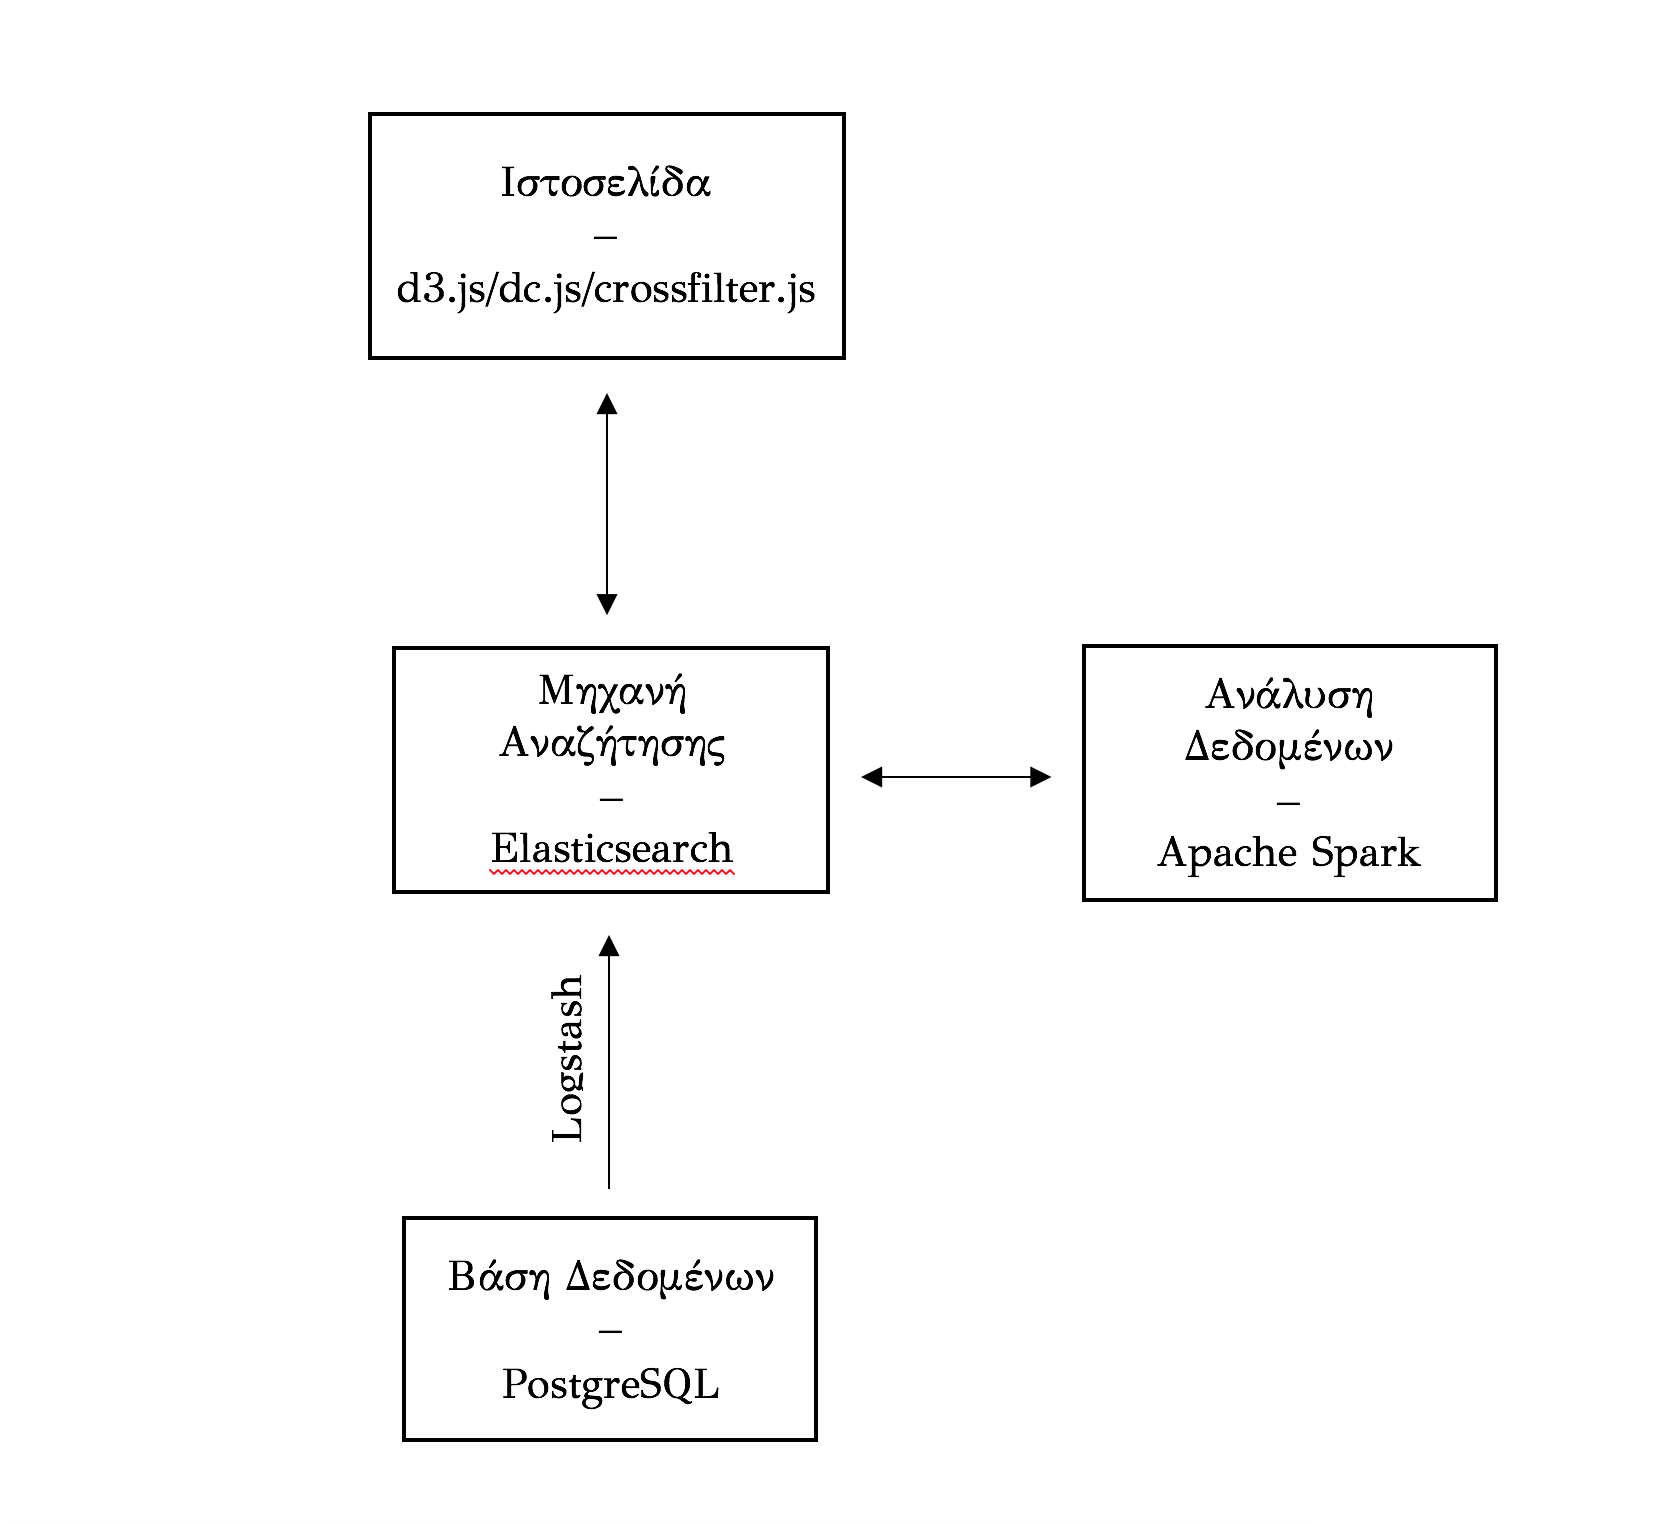
\includegraphics[width=\textwidth]{architecture}
  \label{fig:architecture}
\end{figure}

Τα δεδομένα 

\section{Docker}

Το Visfx είναι φτιαγμένο χρησιμοποιώντας το Docker. Το Docker είναι 

\section{Αποθήκευση και ανάκτηση Δεδομένων}
\subsection{PostgreSQL}
\subsection{Elasticsearch \& Logstash}

\section{Ανάλυση Δεδομέων}

\section{Παρουσίαση \& Απεικόνιση δεδομένων}
\subsection{d3.js, dc.js, crossfilter.js}
\clearemptydoublepage

\chapter{Σενάριο Χρήσης Visfx}\label{ch:chap4}
%!TEX root = ../main.tex



\section{Εισαγωγή}

Ο χρήστης της πλατφόρμας είναι ένας μηχανικός/data scientist ο οποίος δουλεύει σε μια εταιρία που αναπτύσσει μία πλατφόρμα Forex Trading. Αυτός ο μηχανικός δουλεύει πάνω σε ένα Σύστημα Συστάσεων (RS). Ο μηχανικός αυτός έχει στη διάθεση του ένα μεγάλο αριθμό από δεδομένα των συναλλαγών των πελατών τα οποία θέλει να αξιοποιήσει στο RS που υλοποιεί. Με άλλα λόγια έχει στη διάθεση του ένα σύνολο από έμμεσες αξιολογήσεις, από τις οποίες θα χρειαστεί να εξάγει κάποιες «ψευδο-αξιολογήσεις» με τις οποίες θα εκπαιδευτεί το RS.

Όπως αναφέραμε και προηγουμένως η εξαγωγή των ψευδο-αξιολογήσεων μπορεί να χωριστεί σε τρία στάδια:

\begin{enumerate}
	\item Ανάλυση και δημιουργία «διαισθήσεων» πάνω στα δεδομένα
	\item Επιλογή των χαρακτηριστικών των δεδομένων για τον υπολογισμό των ψευδο-αξιολογήσεων και αξιολόγηση των ψευδο-αξιολογήσεων
	\item Αξιολόγηση των αποτελεσμάτων του Συστήματος Συστάσεων \ldots
\end{enumerate} 	

Έτσι και το Visfx χωρίζεται αντίστοιχα σε τρεις ενότητες, στην Data Overview, Feature Selection, και Recommendations.

\section{Επισκόπηση Δεδομένων – Data Overview}

Ξεκινώντας στην καρτέλα Data Overview ο μηχανικός μπορεί να διαλέξει την χρονική περίοδο πάνω στην οποία θέλει να δουλέψει. Αρχικά χαιρετίζεται με ένα Parallel Coordinates διάγραμμα μέσω του οποίου μπορεί γρήγορα και αποτελεσματικά να δει το σύνολο των δεδομένων του και να κάνει οπτικοποιημένες αναζητήσεις πάνω σ’ αυτά. Ο χρήστης μπορεί να είτε να φιλτράρει τους άξονες μαρκάροντας περιοχές πάνω σ’ αυτούς, είτε να χρησιμοποιήσει τα πεδία αμέσως κάτω από το διάγραμμα. Κάθε γραμμή στο διάγραμμα αναπαριστά μία συναλλαγή, ενώ οι γραμμές με το ίδιο χρώμα είναι συναλλαγές από την ίδια χώρα. Για παράδειγμα ξεκινώντας από τα αριστερά βλέπουμε ότι ο Provider με ID 911888 που είναι από την Σιγκαπούρη άνοιξε μία συναλλαγή XAU/USD την τάδε ημερομηνία, έκλεισε την δείνα με μικρό Amount και το Net PnL ήταν μικρό αλλά αρνητικό.

\begin{figure}[H]
  \centering
  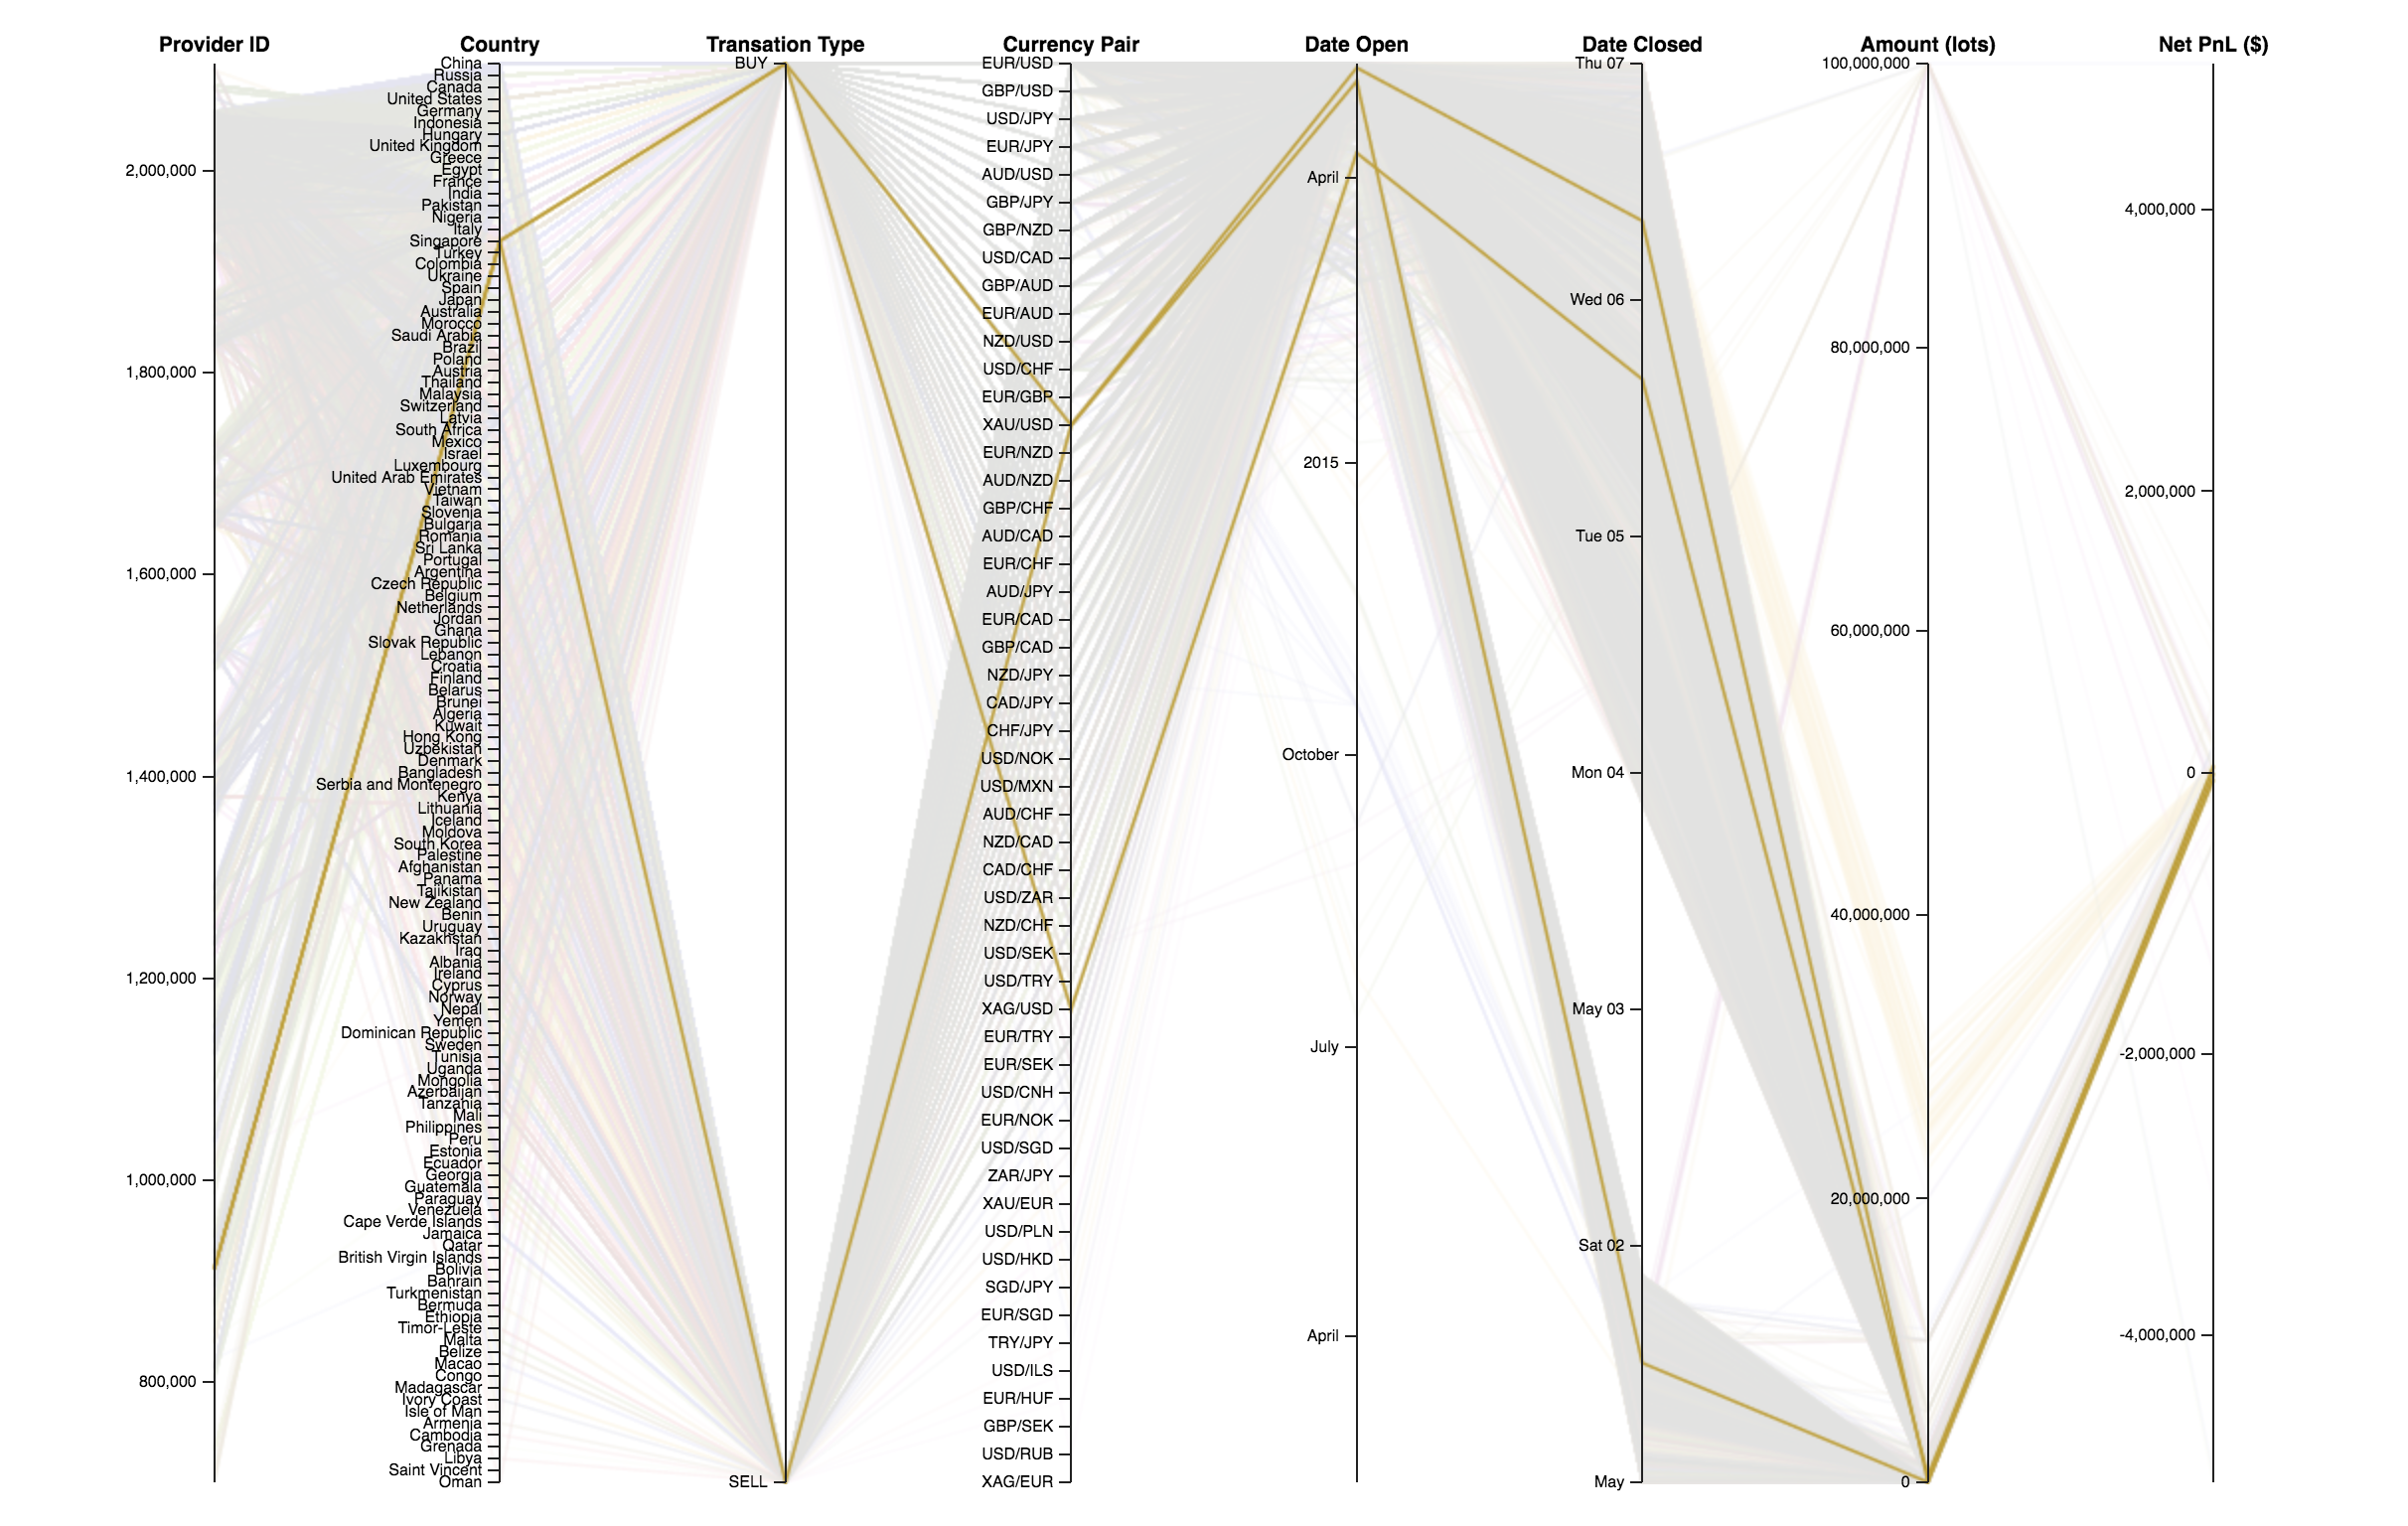
\includegraphics[width=\textwidth]{parcoords_single}
  \label{fig:parcoords_single}
\end{figure}

Επίσης ο χρήστης μπορεί να κάνει πιο περίπλοκες αναζητήσεις. Για παράδειγμα μπορεί να επιλέξει πάνω στους άξονες τις συναλλαγές που έγιναν από τις Ηνωμένες Πολιτείες της Αμερικής στο ζεύγος GBP/USD και USD/CAD και άνοιξαν μέσα στον Απρίλιο:

\begin{figure}[H]
  \centering
  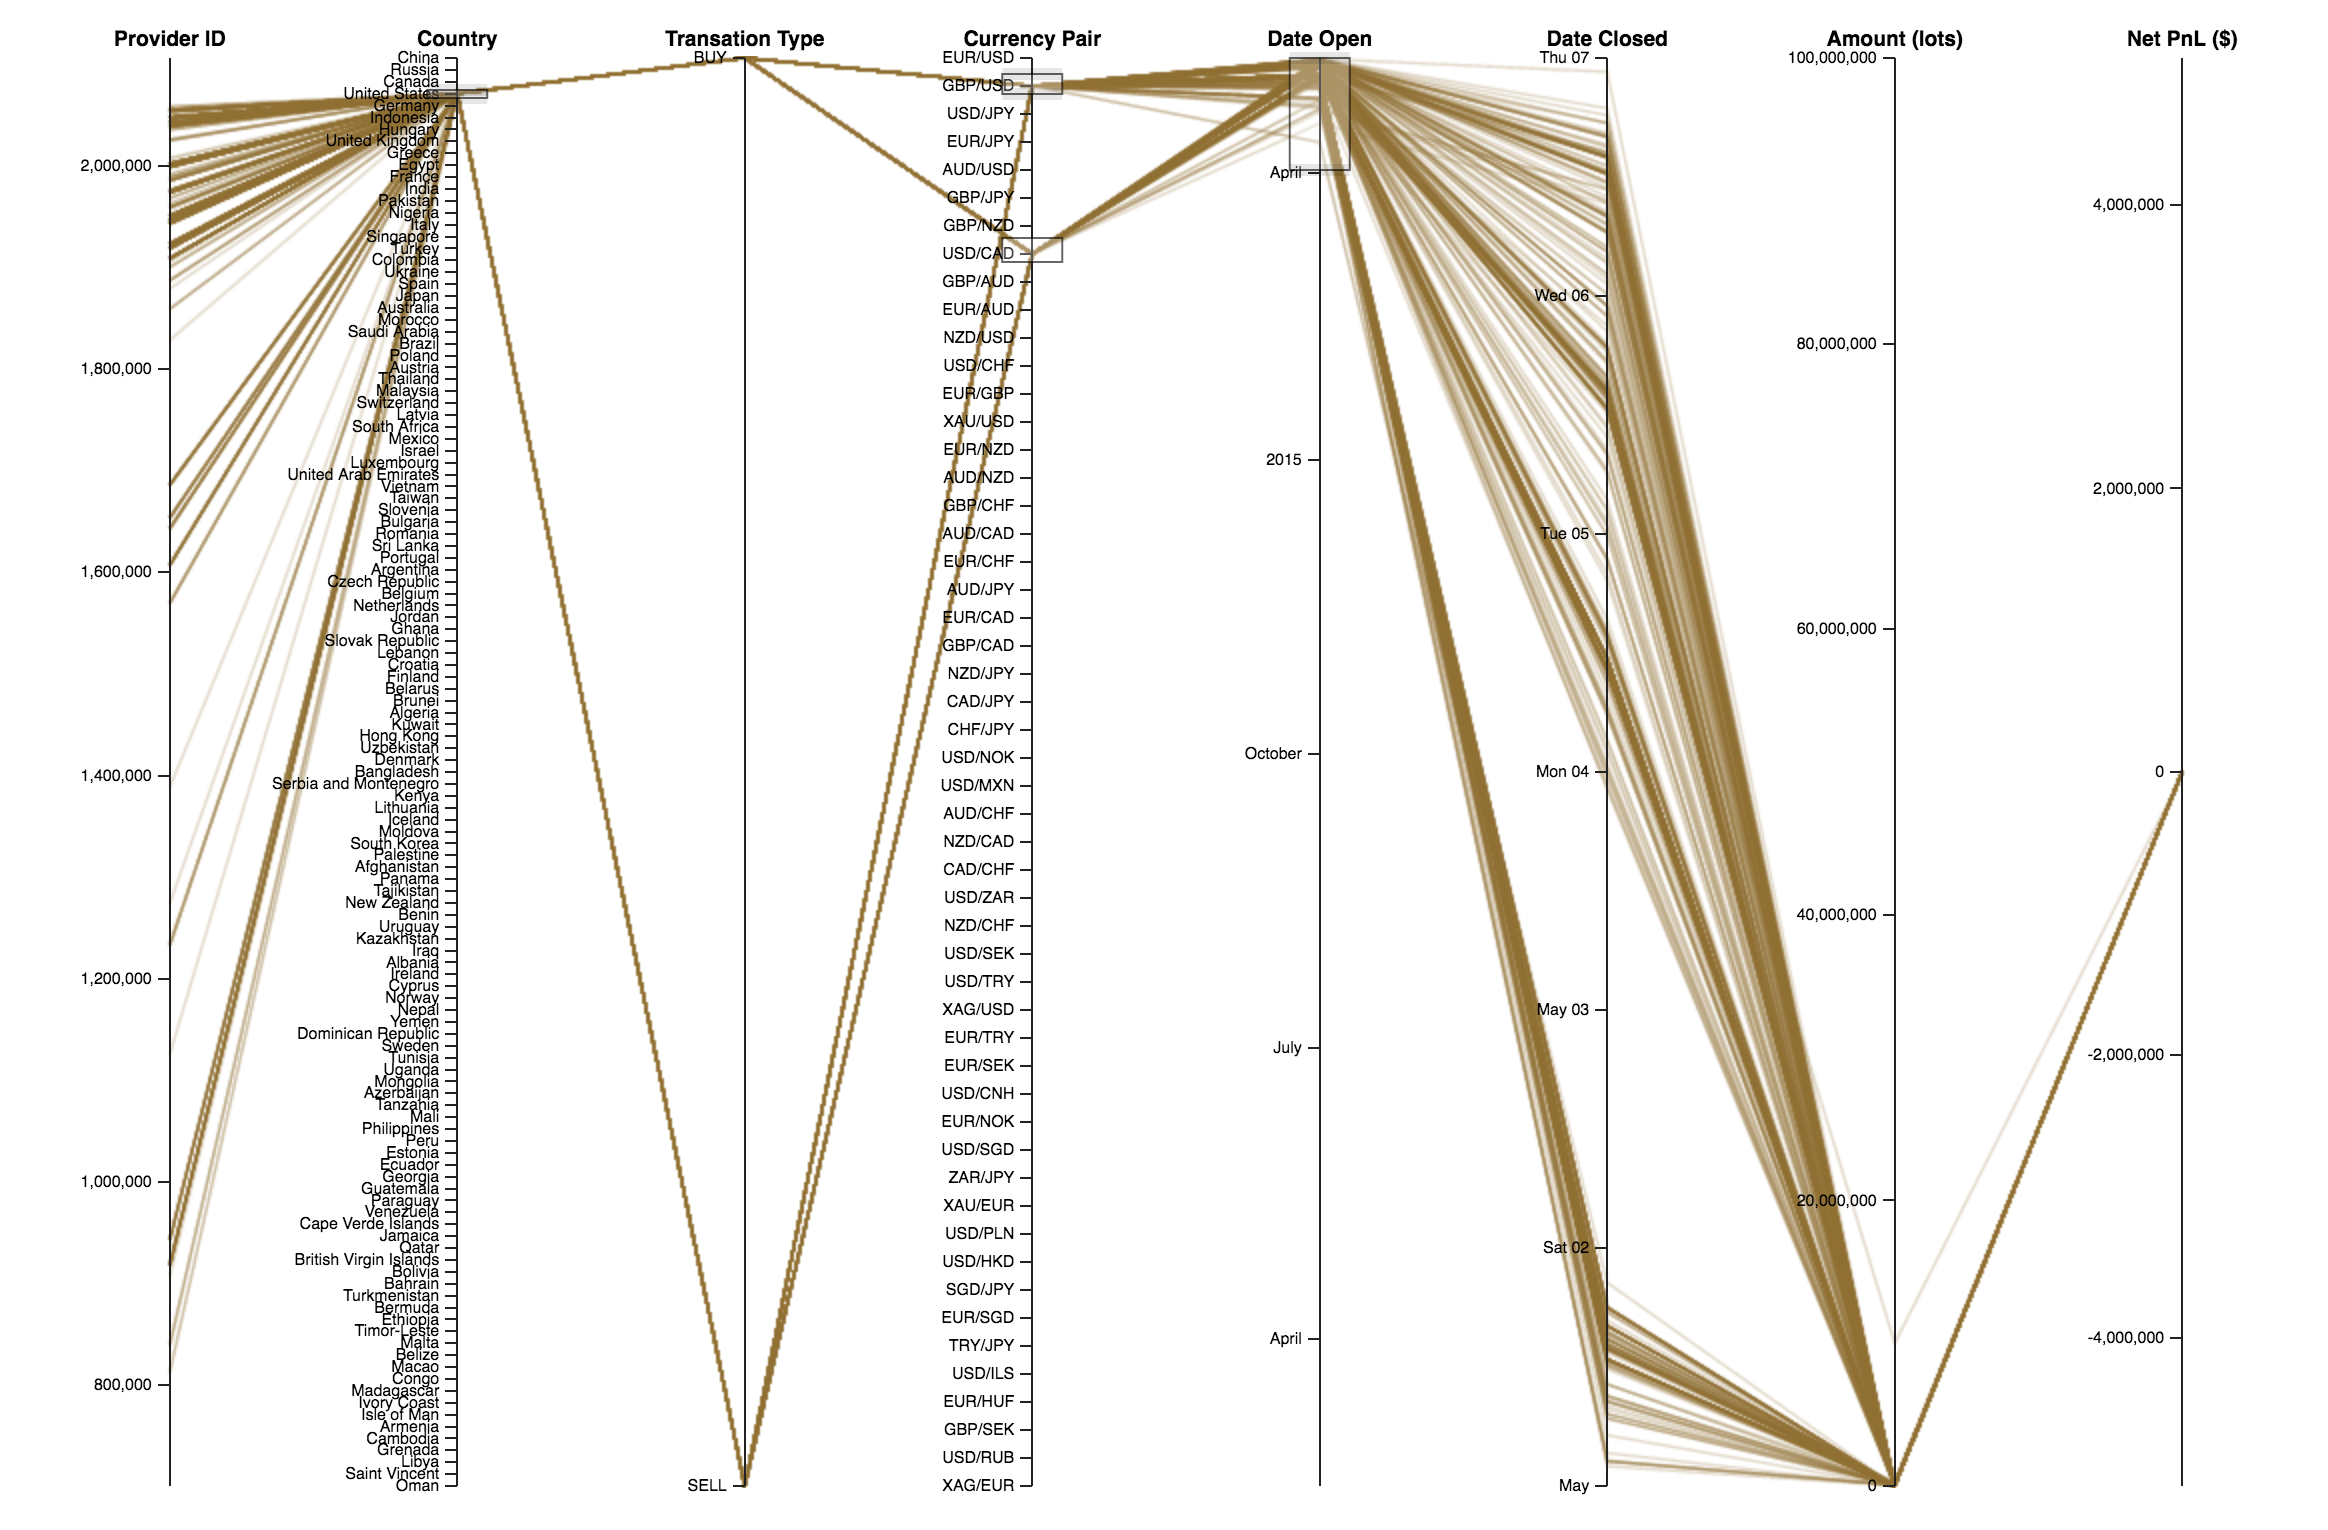
\includegraphics[width=\textwidth]{parcoords_complex}
  \label{fig:parcoords_complex}
\end{figure}

Κάνοντας αυτή την αναζήτηση μπορεί να δει πως συμπεριφέρονται οι χρηματιστές σε μία χώρα όταν συναλλάσσονται ένα συγκεκριμένο ζεύγος και ρυθμίζονται το παράθυρο του Date Open να δει πως η διάρκεια της συναλλαγής επηρεάζει τα κέρδη της.

Επεκτείνοντας περισσότερο, αν δούμε τις συναλλαγές για το ζεύγος EUR/USD βλέπουμε ότι αυτές που είχαν μικρότερη διάρκεια ήταν αρκετά πιο κερδοφόρες απ’ αυτές με διάρκεια πάνω από εβδομάδα. Γι’ αυτό επιλέξαμε στη συνέχεια σαν χαρακτηριστικό την διάρκεια των συναλλαγών (Trade Duration)

\begin{figure}[H]
  \centering
  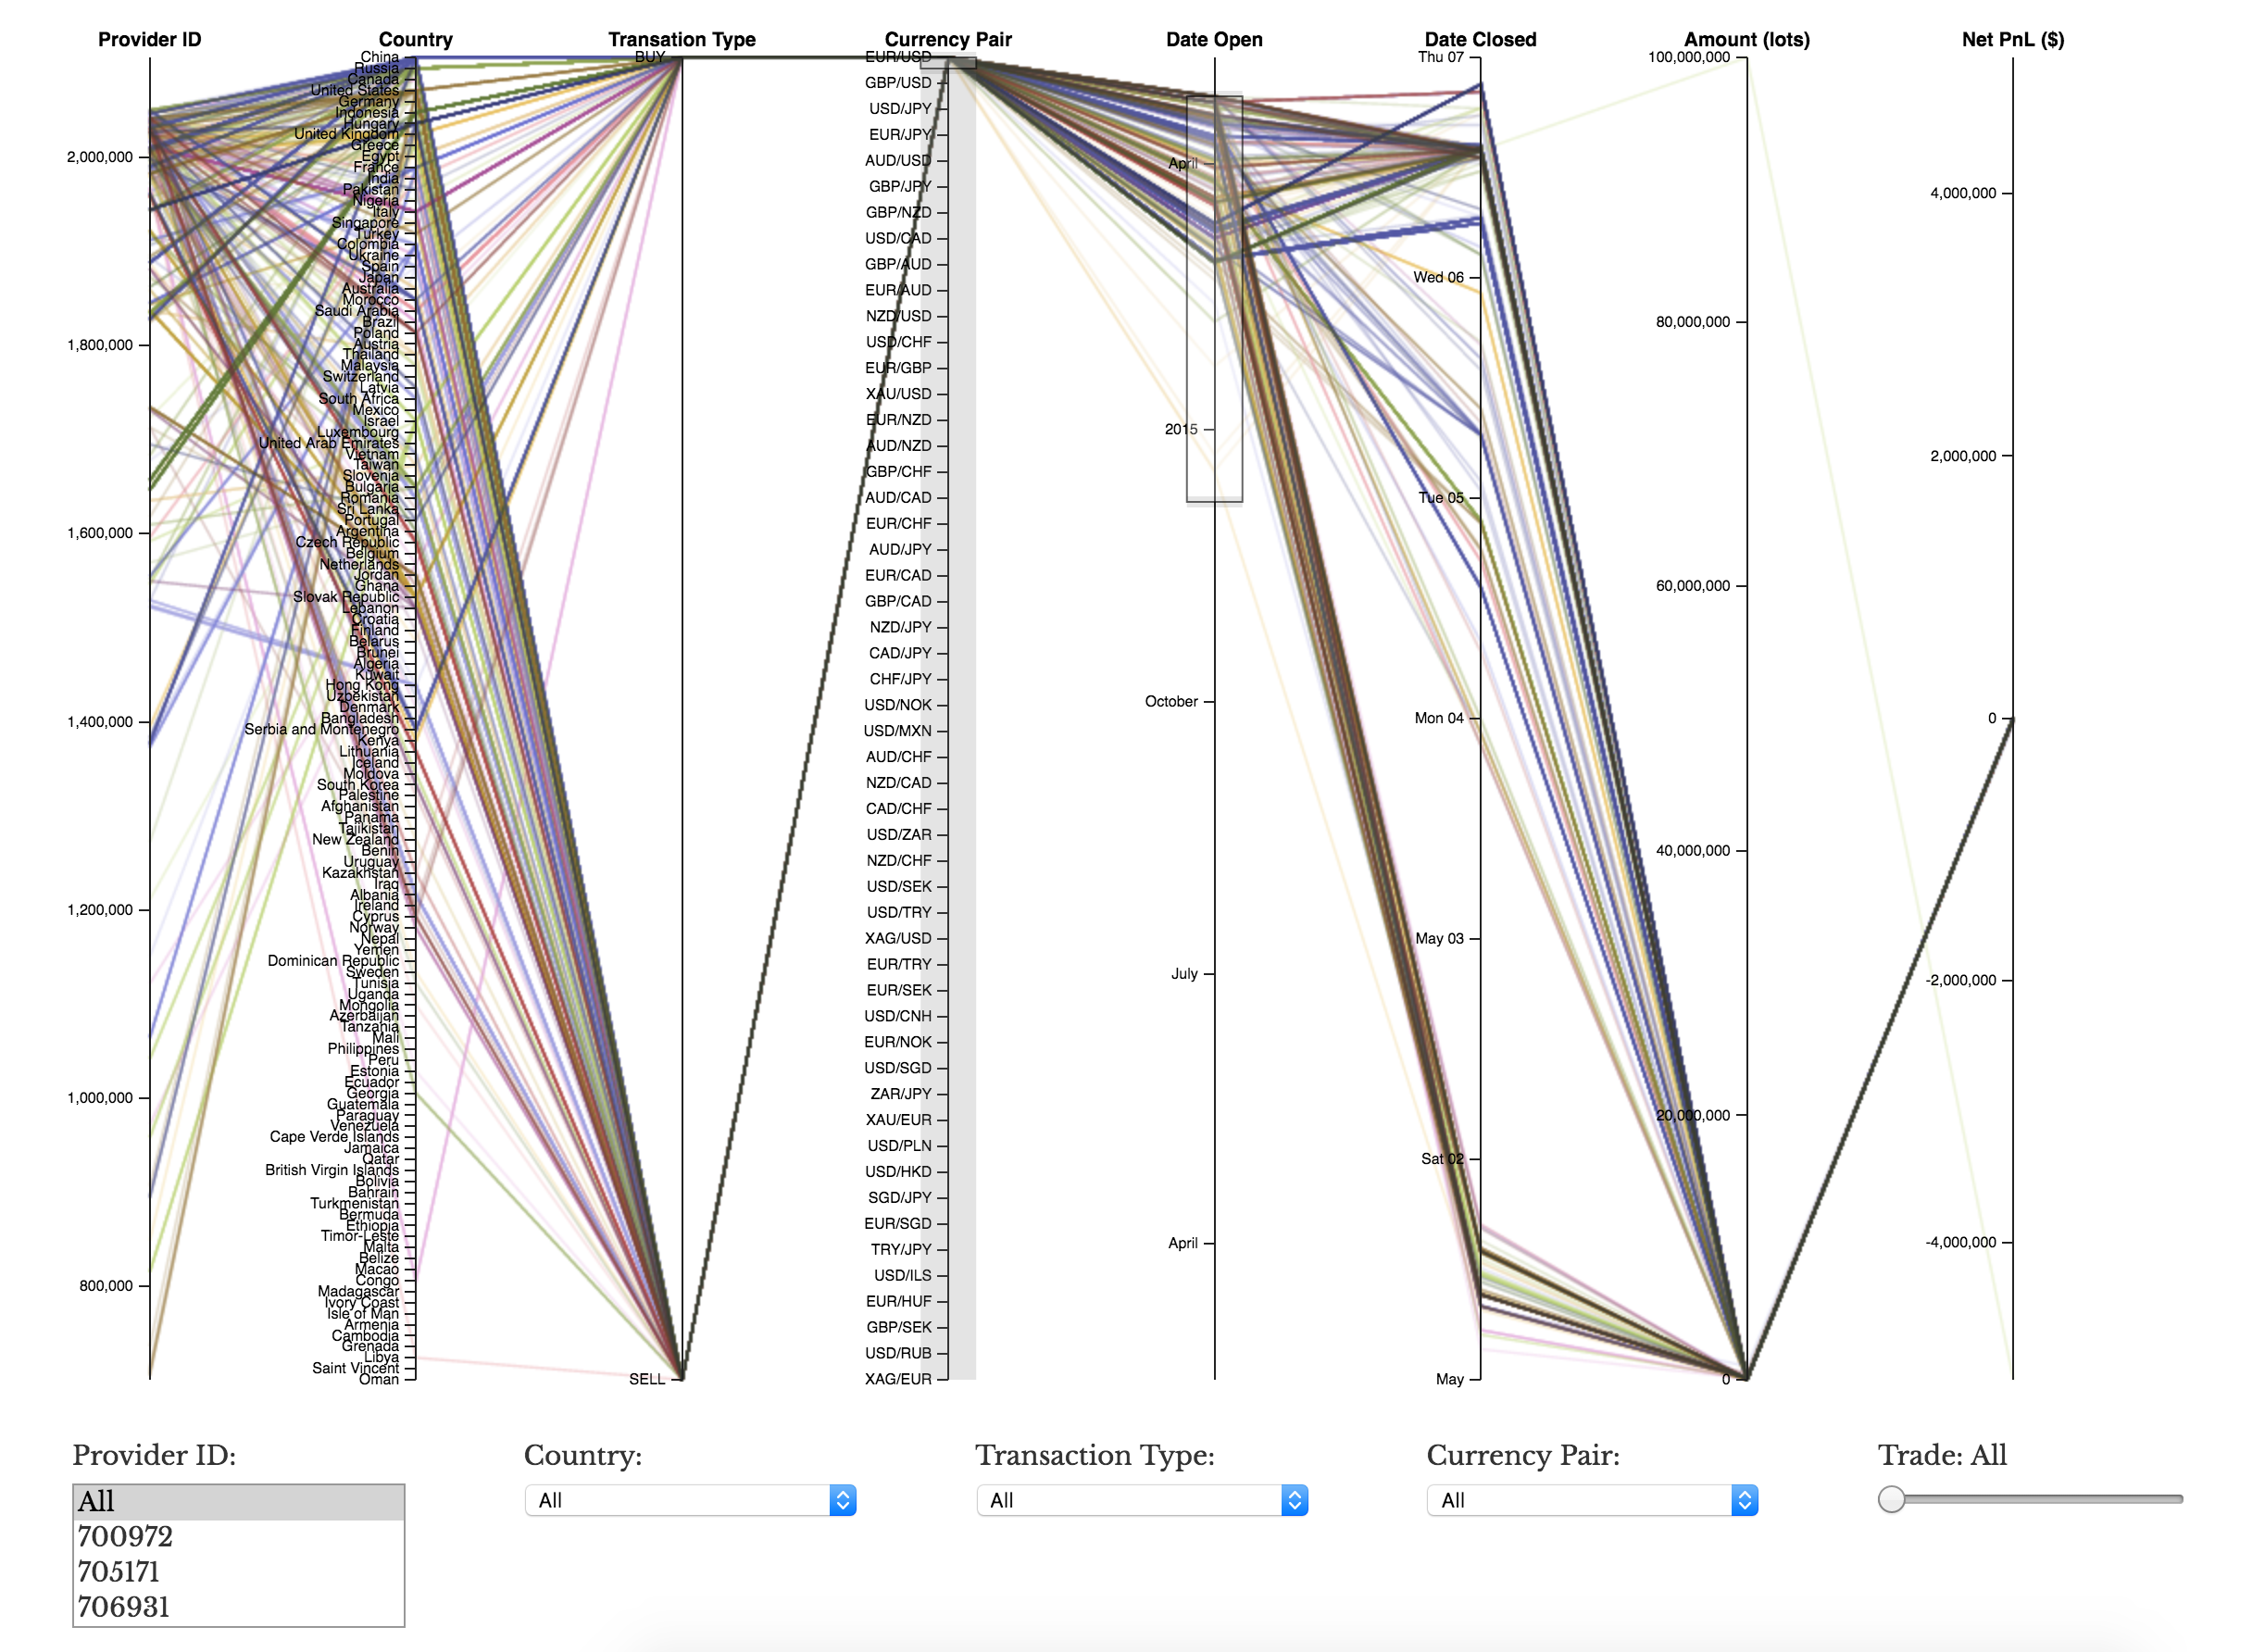
\includegraphics[width=\textwidth]{parcoords_late}
  \label{fig:parcoords_late}
\end{figure}
\hfill
\begin{figure}[H]
  \centering
  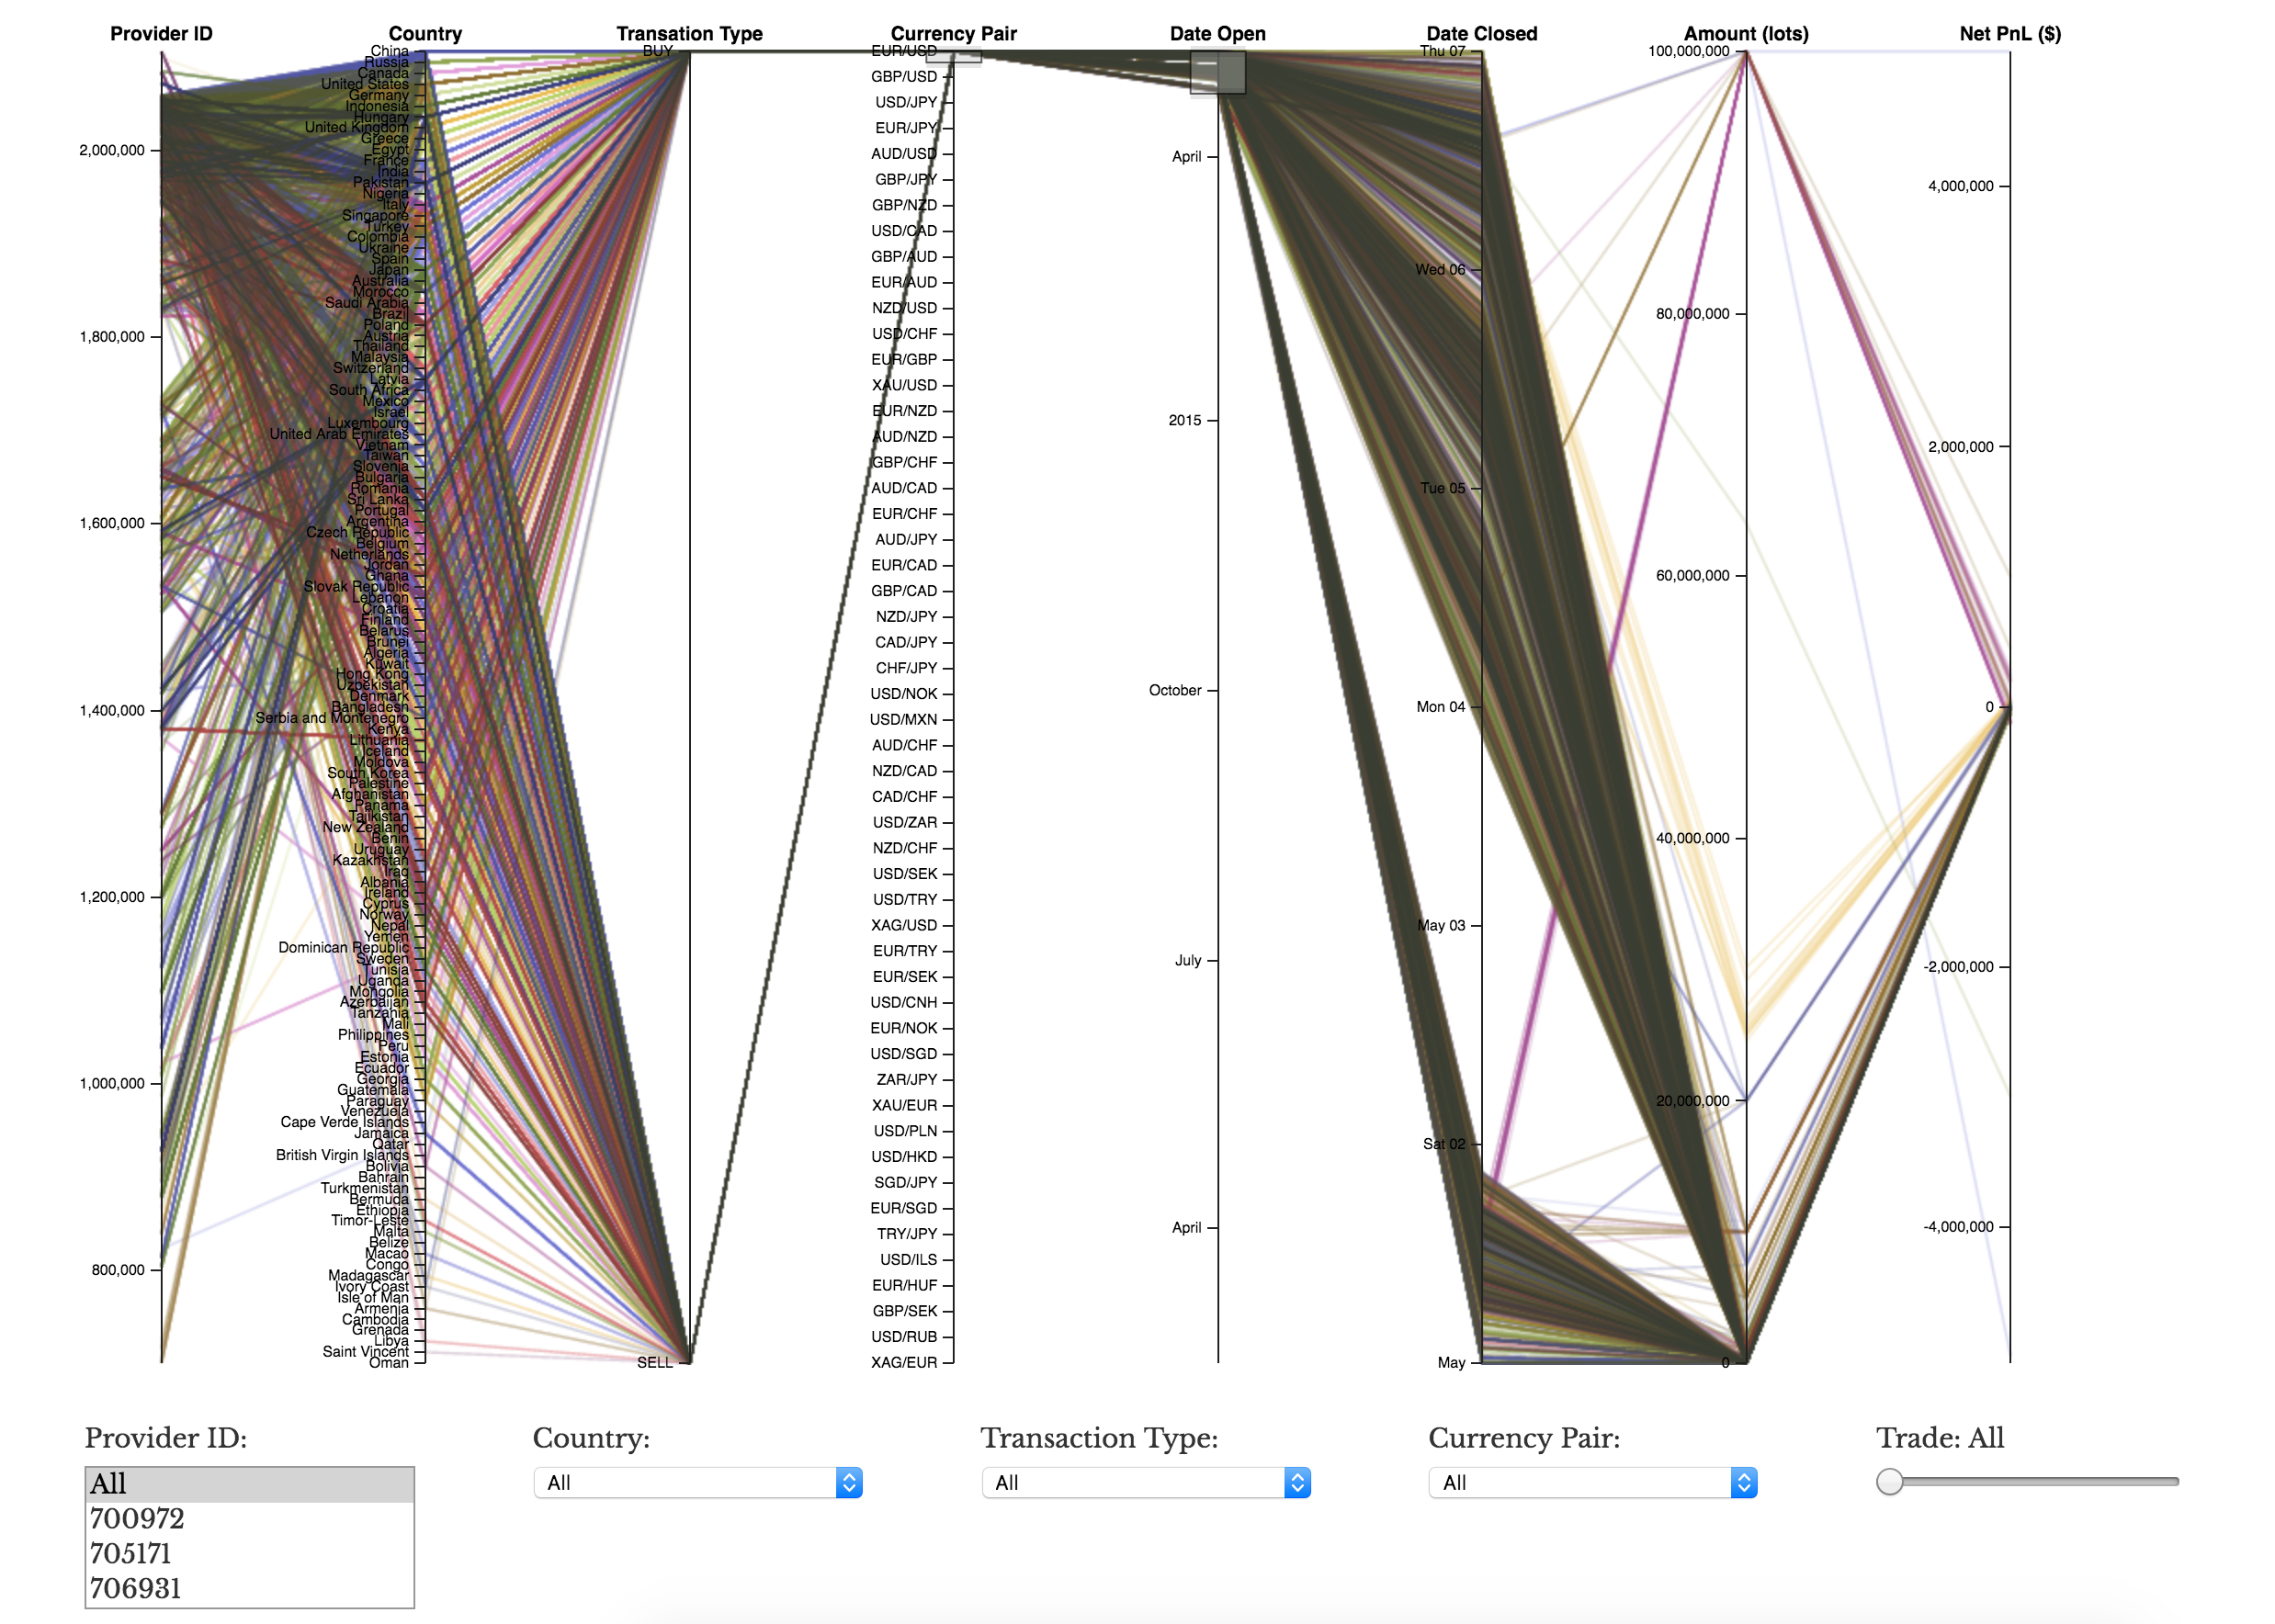
\includegraphics[width=\textwidth]{parcoords_early}
  \label{fig:parcoords_early}
\end{figure}

Στη συνέχεια ο χρήστης μπορεί δει πιο αναλυτικά πτυχές των δεδομένων μέσω των επόμενων γραφημάτων.

\begin{figure}[H]
  \centering
  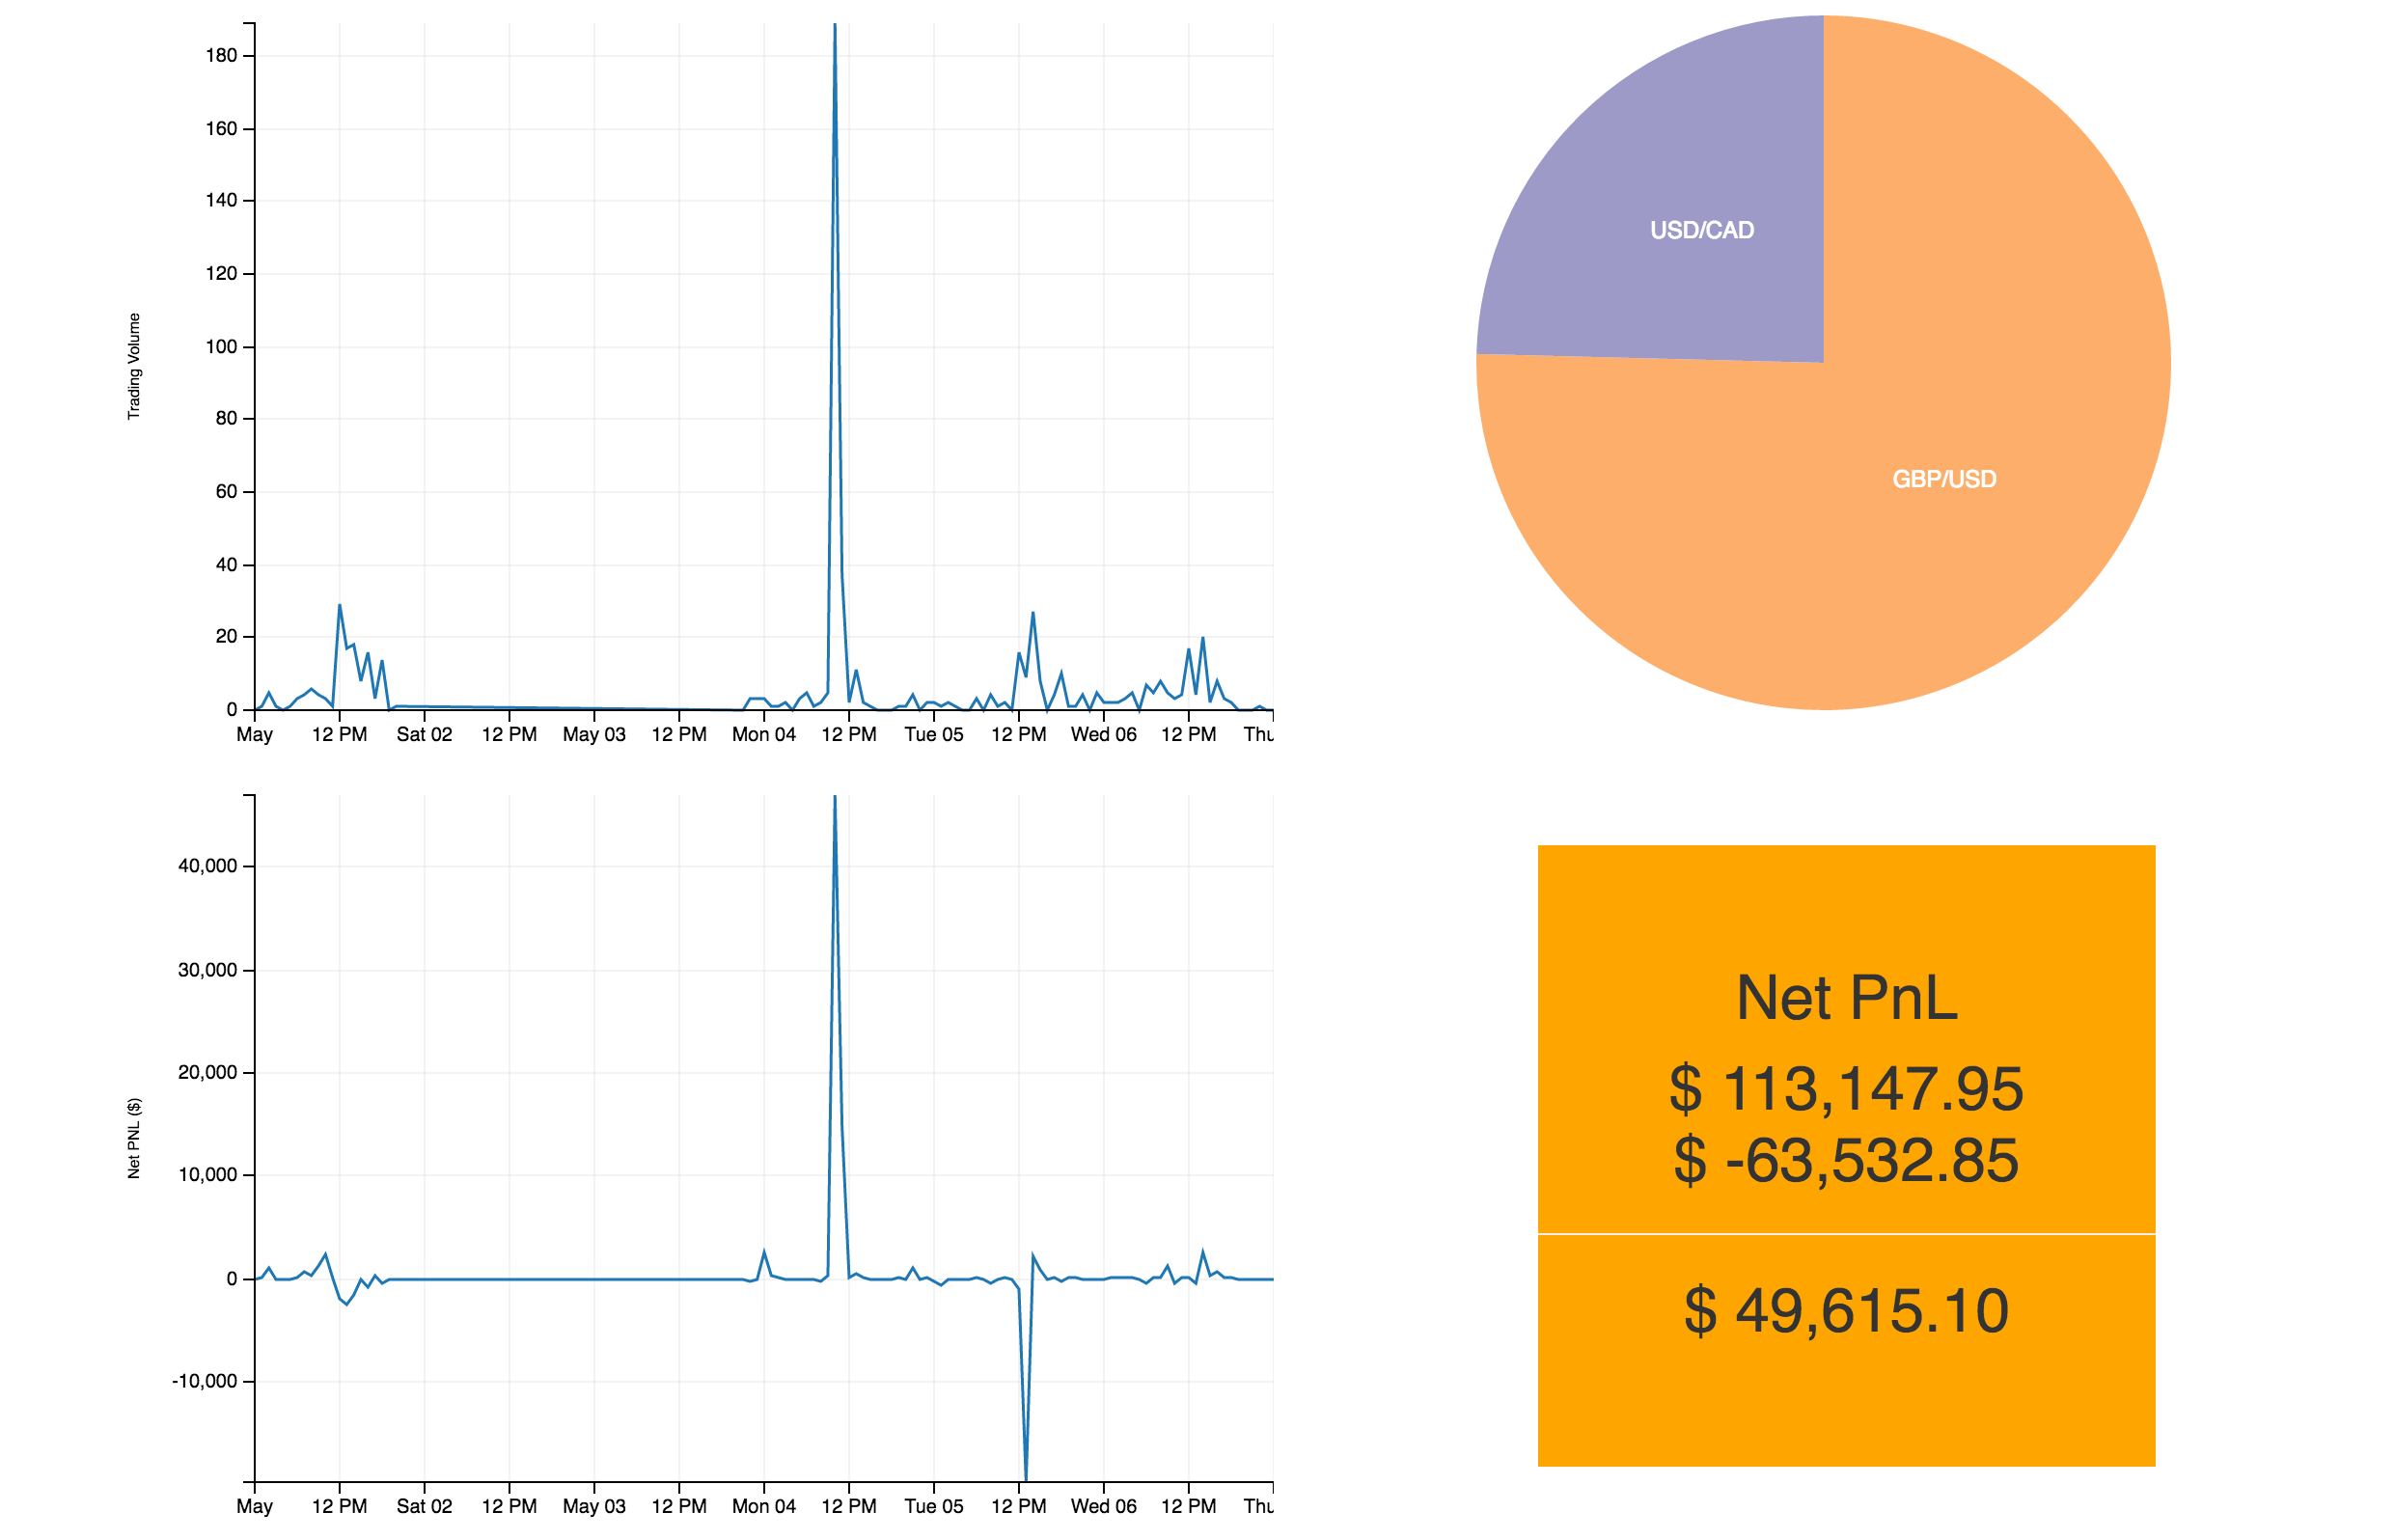
\includegraphics[width=\textwidth]{overview_1}
  \label{fig:overview_1}
\end{figure} 

\begin{figure}[H]
  \centering
  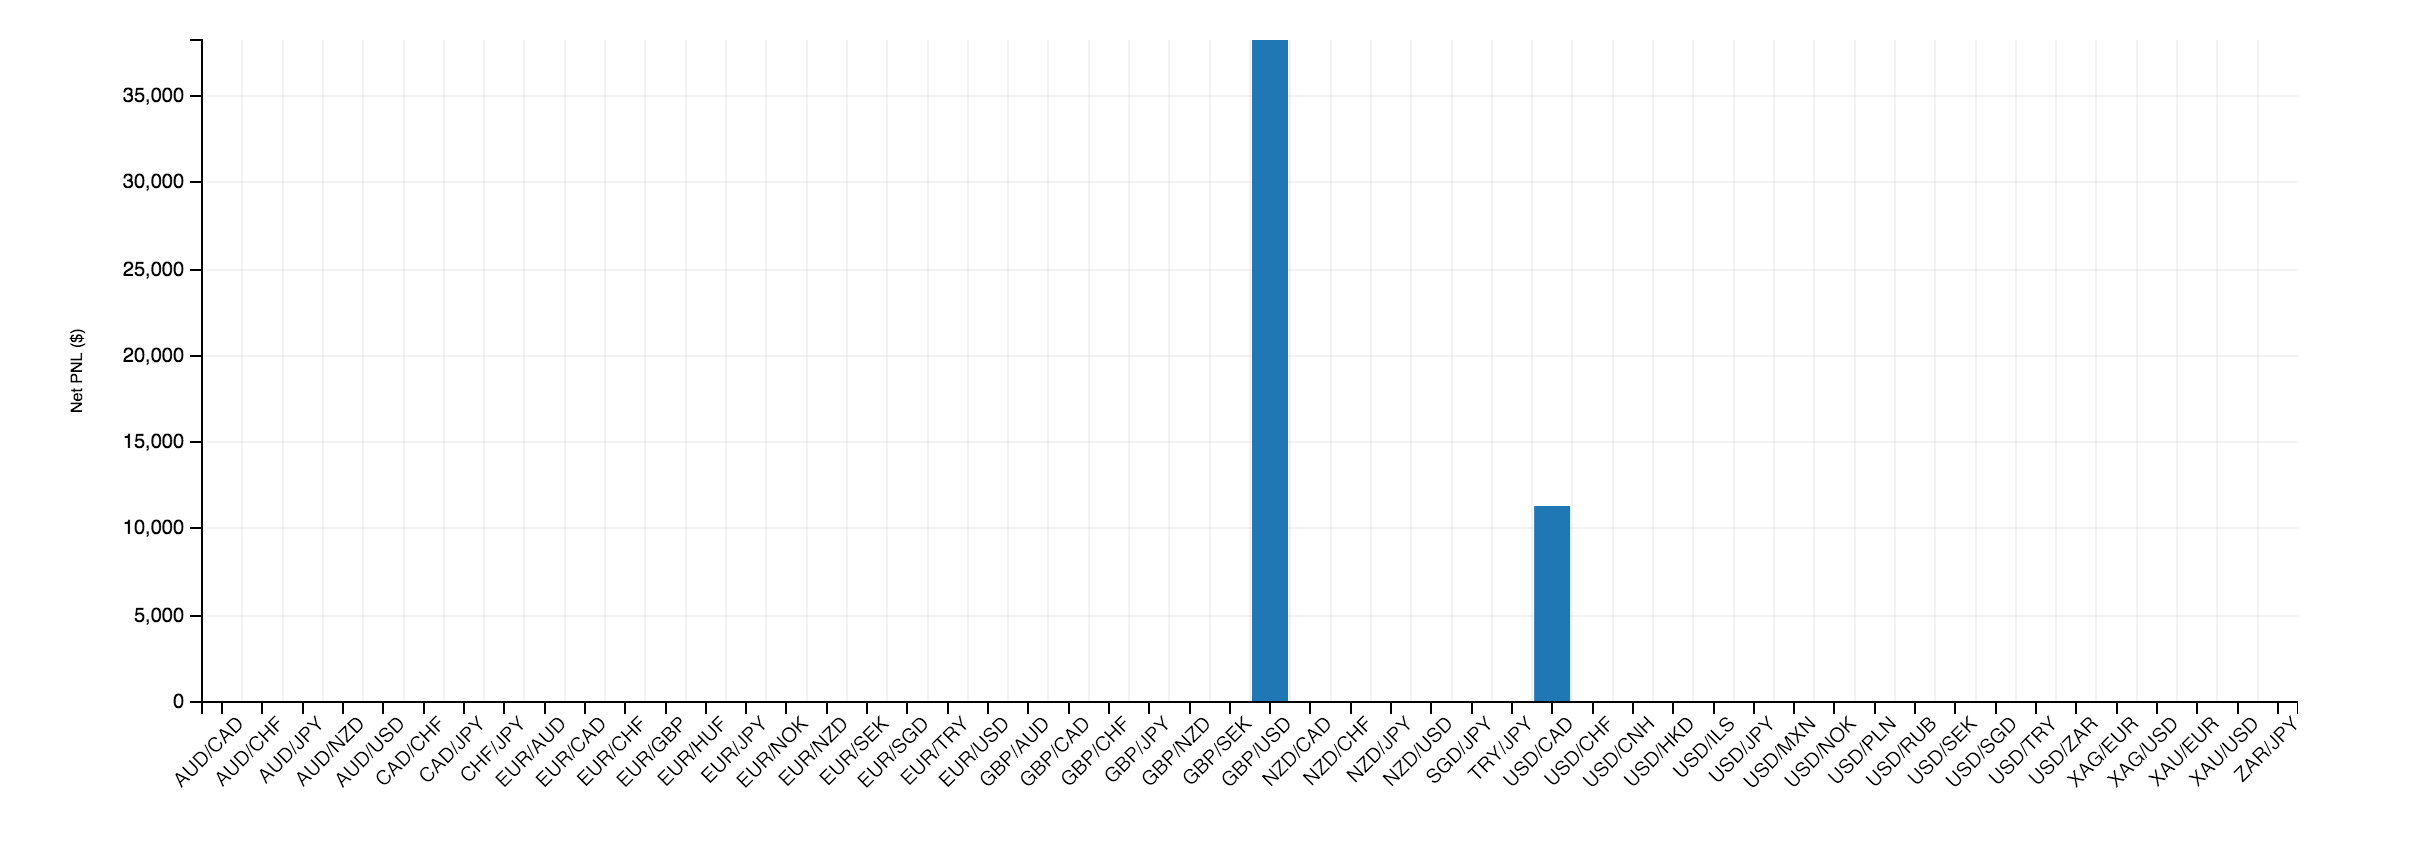
\includegraphics[width=\textwidth]{overview_2}
  \label{fig:overview_2}
\end{figure}

\begin{figure}[H]
  \centering
  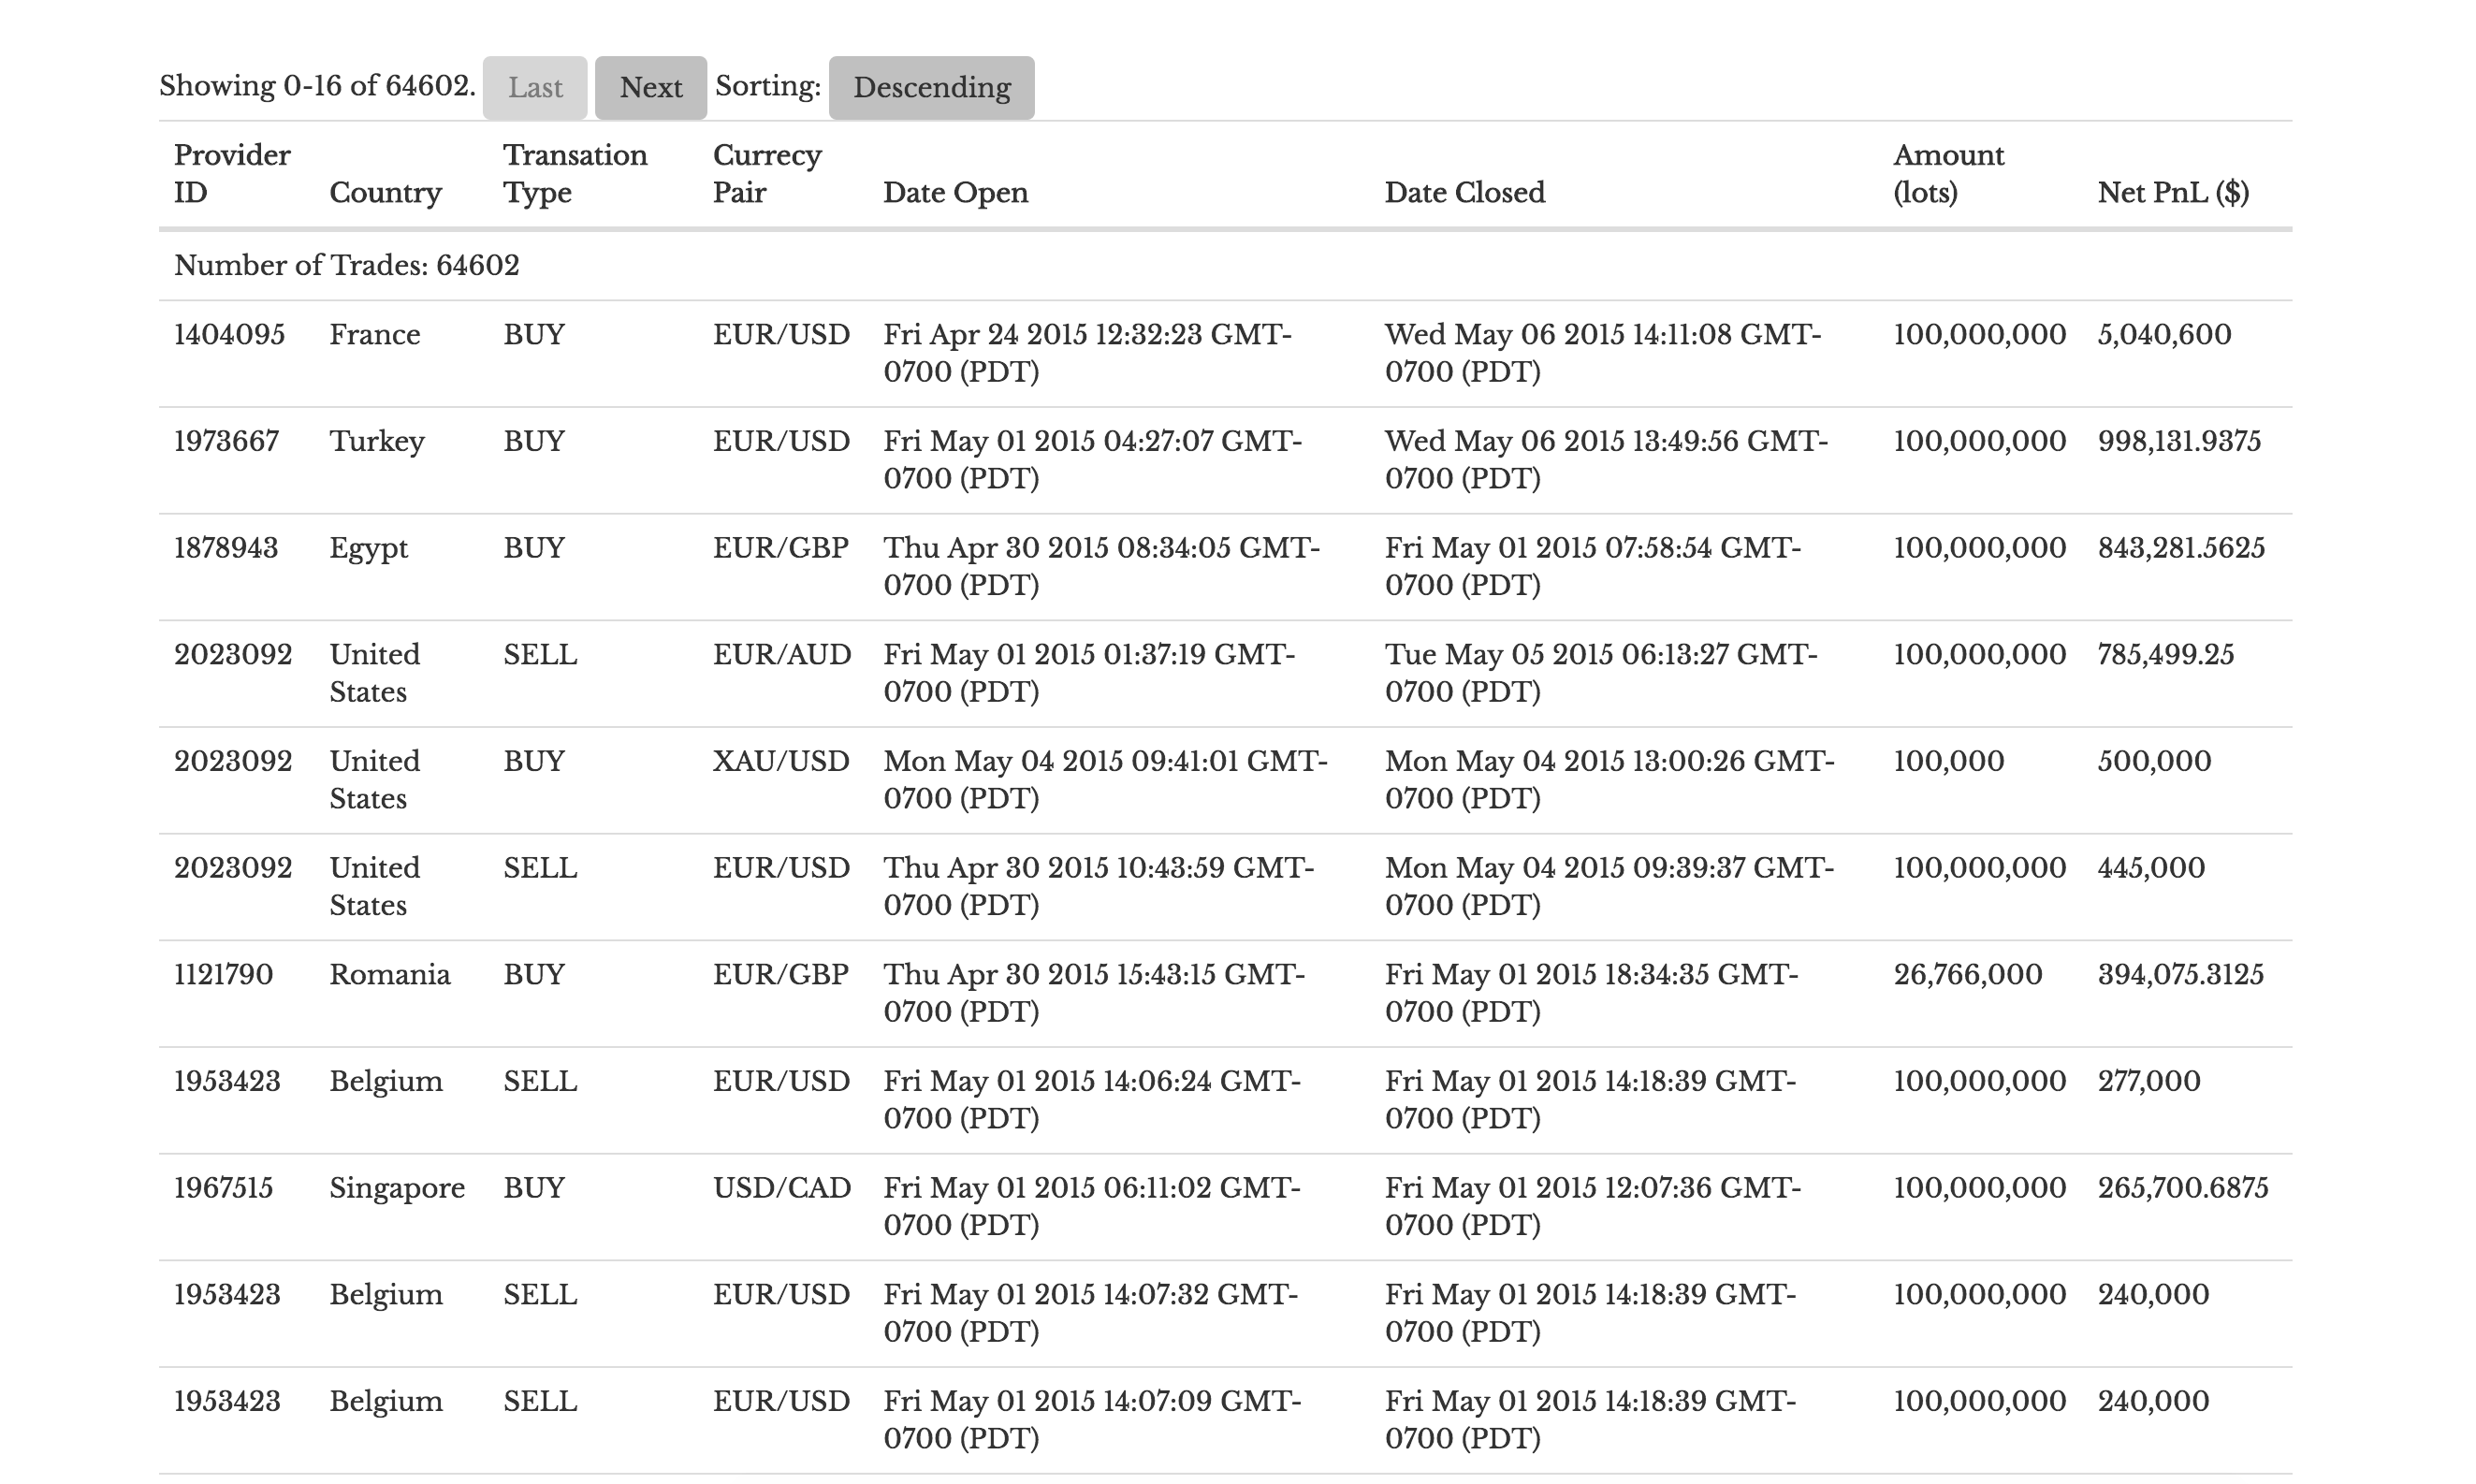
\includegraphics[width=\textwidth]{overview_3}
  \label{fig:overview_3}
\end{figure}

Τα διαγράμματα έχουν προσαρμοστεί και δείχνουν για παράδειγμα ποια ήταν τα νομισματικά ζεύγη που συναλλασσόταν αυτή τη στιγμή, πώς ήταν μοιρασμένα τα κέρδη και οι ζημιές ανά ζεύγος. Από τον πίνακα στο τέλος βλέπουμε ότι αυτή η αύξηση προήλθε κυρίως από μία κακή συναλλαγή ενός χρηματιστή που έχασε περίπου 5 εκατομμύρια δολάρια.

Έτσι μπορεί να δει οι συναλλαγές αυτές πότε έγιναν, ποιες ήταν επικερδείς και ποιες όχι, και πόσα χρήματα κινήθηκαν σ’ αυτές. Αντίστοιχα μπορεί να κάνει επιλογές πάνω σ’ αυτές τις απεικονίσεις και να δει πιο συγκεκριμένες πλευρές των δεδομένων του. 

Μ’ αυτό τον τρόπο μπορεί να αρχίσει να καταλαβαίνει ποια χαρακτηριστικά των συναλλαγών είναι πιο σημαντικά και μπορούν να χρησιμοποιηθούν για να εξαχθούν οι ψευδο-αξιολογήσεις. Για παράδειγμα: Ποια ζευγάρια βγάζουν το περισσότερο κέρδος; Oι συναλλαγές που έχουν μικρή διάρκεια – η διαφορά ανάμεσα στην ώρα ανοίγματος και κλεισίματος συναλλαγής – είναι καλύτερες ή χειρότερες; Τι σχέση παίζει ο αριθμός των συναλλαγών που γίνονται σε έναν ζεύγος;

Για παράδειγμα:

\begin{figure}[H]
	\centering
	\begin{minipage}{0.3\textwidth}
		\centering
		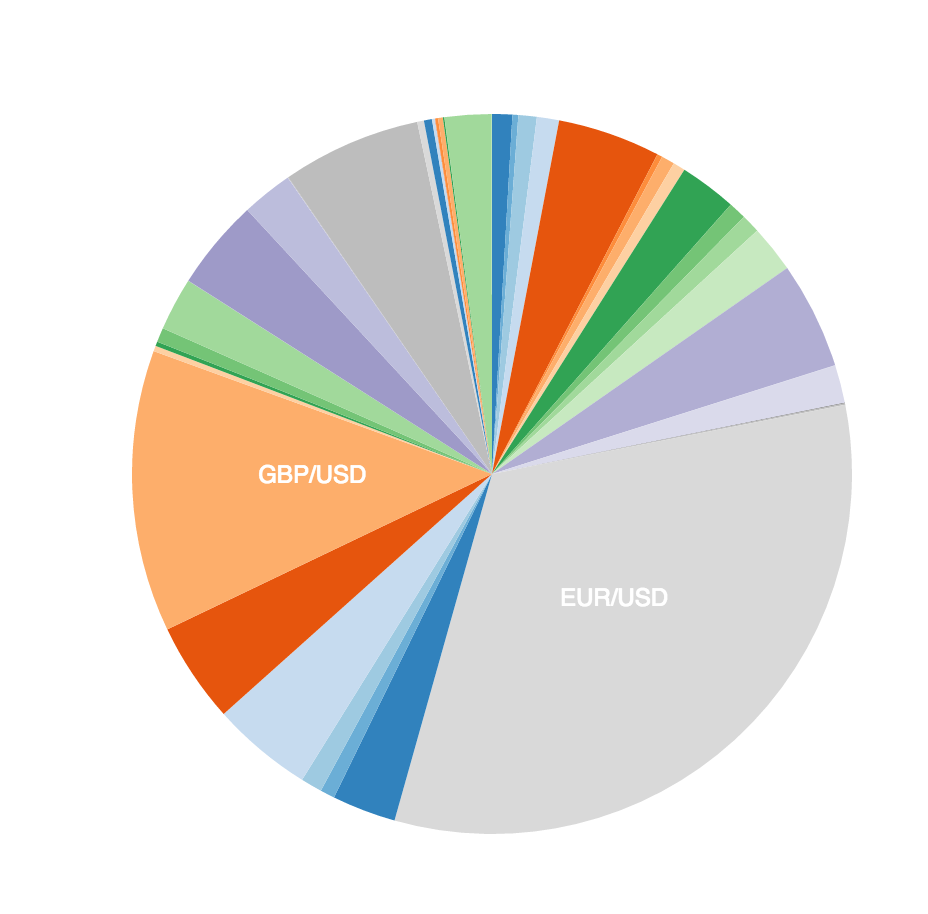
\includegraphics[width=\textwidth]{overview_4}
		\label{fig:overview_4}	
	\end{minipage}
	\hfill
	\begin{minipage}{0.7\textwidth}
		\centering
		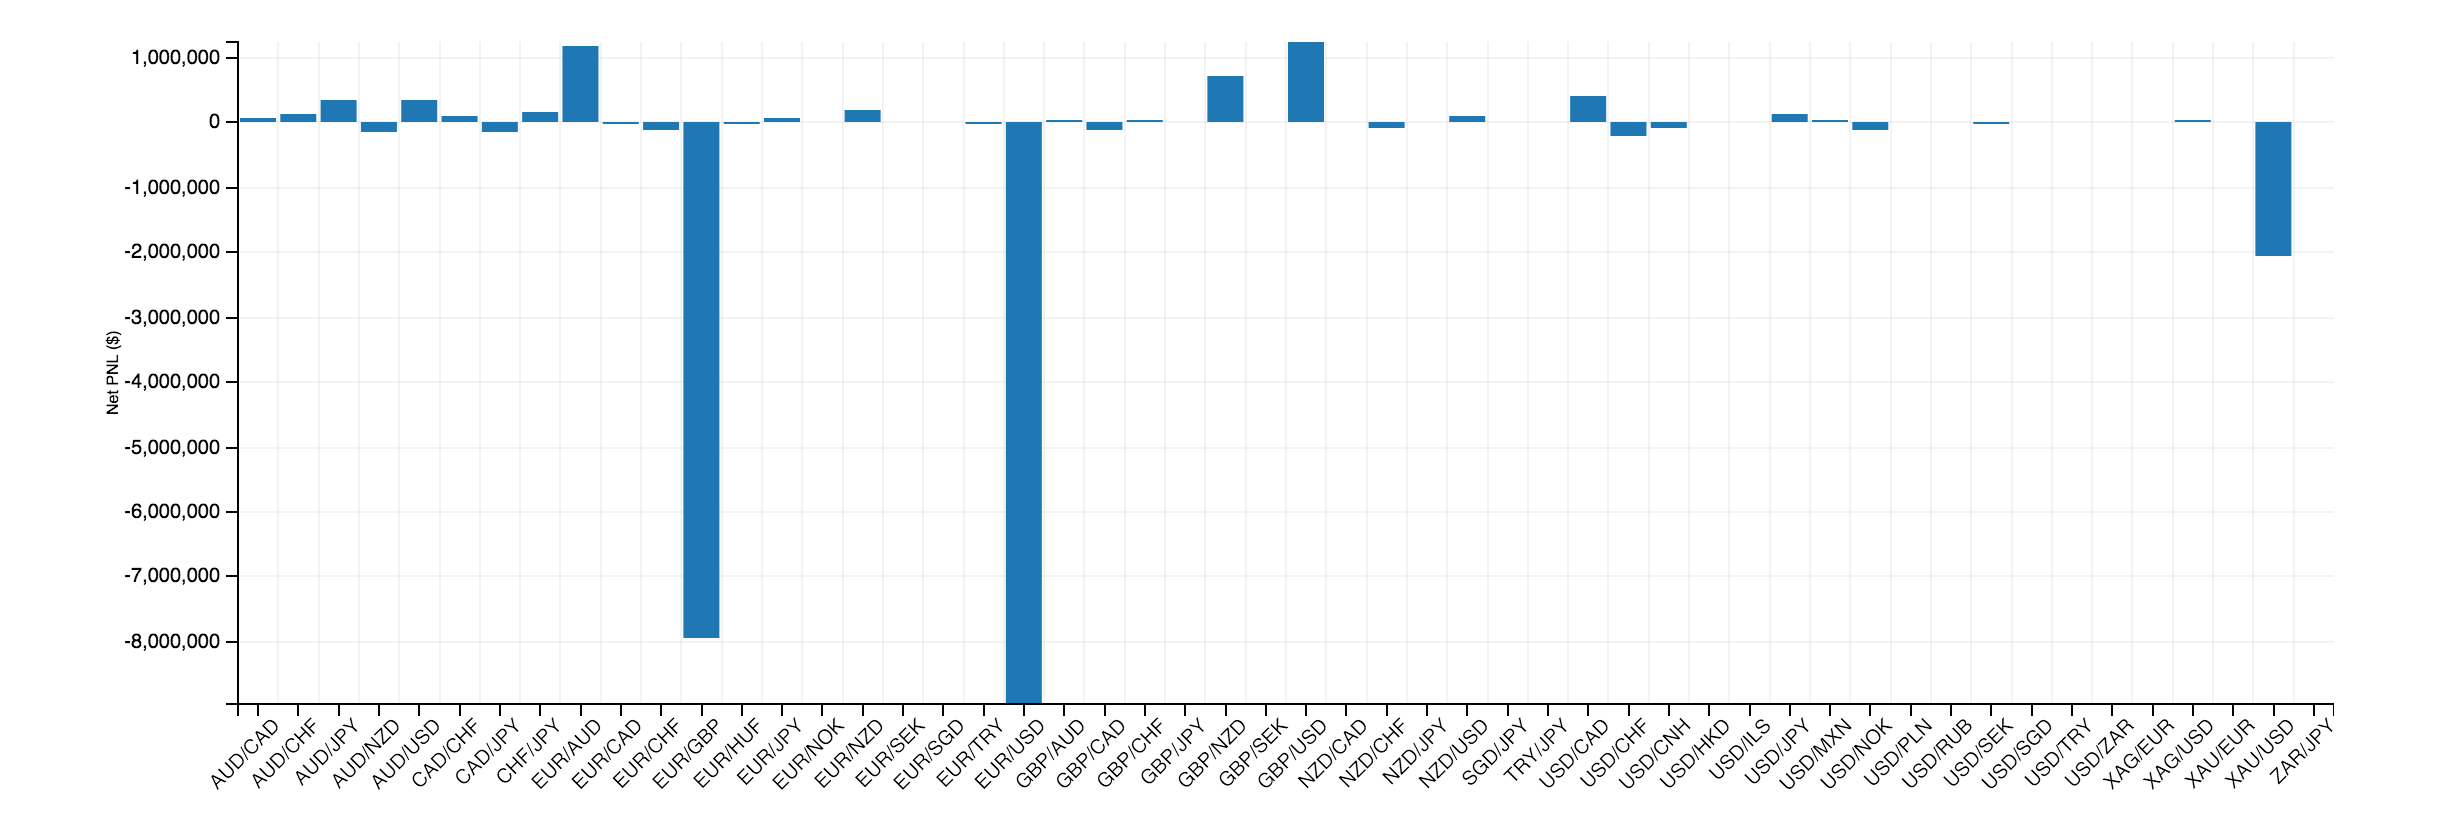
\includegraphics[width=\textwidth]{overview_5}
		\label{fig:overview_5}	
	\end{minipage}
\end{figure}

Βλέπουμε από το τελευταίο ραβδόγραμμα ότι τα ζεύγη που βγάζουν συνολικά το περισσότερο κέρδος αυτή την περίοδο είναι τα GBP/USD, EUR/AUD και GBP/NZD, ενώ οι περισσότερες ζημιές έχουν έρθει από τα EUR/USD, EUR/GBP και XAU/USD. Από την άλλη, τα ζεύγη που συναλλάχθηκαν περισσότερο είναι τα EUR/USD, GBP/USD, USD/JPY και EUR/JPY. Παρατηρούμε ότι παρόλο που το EUR/USD έχει τις περισσότερες ζημιές οι χρηματιστές το επιλέγουν τις περισσότερες φορές. Αν δούμε όμως αναλυτικά τις συναλλαγές και τις συγκρίνουμε μ’ αυτές του GBP/USD θα δούμε ότι στο EUR/USD οι καλύτερες συναλλαγές έχουν σημαντικά περισσότερα κέρδη απ’ ότι στο GBP/USD. Αυτό μας δείχνει ότι τα κέρδη (PnL) δεν μπορεί να είναι το αποκλειστικό χαρακτηριστικό για την αξιολόγηση μίας συναλλαγής. Ο αριθμός των συναλλαγών (Trade Count) μπορεί να περιέχει περισσότερη πληροφορία, γιατί ο χρηματιστής που έχει απ’ ευθείας γνώση της αγοράς επέλεξε συνειδητά να συναλλαχθεί το νομισματικό ζεύγος. Έτσι στη συνέχεια επιλέγουμε ως χαρακτηριστικά το Net PnL και το Trade Count μαζί με το Trade Duration.

\section{Επιλογή Χαρακτηριστικών – Feature Selection}

Αφού ο προγραμματιστής καταλήξει στα χαρακτηριστικά που θα χρησιμοποιήσει μπορεί να τα υλοποιήσει προγραμματιστικά και στη συνέχεια να τα δώσει πίσω στο Visfx ώστε να τα οπτικοποιήσει. 

Στη δικιά μας ανάλυση χρησιμοποιήσαμε τέσσερεις ομάδες χαρακτηριστικών: χαρακτηριστικά ανά συναλλαγή, ανά χρηματιστή, ανά νόμισμα, και ανά χώρα. Σε κάθε μία απ’ αυτές τις ομάδες χρησιμοποιήσαμε τα εξής χαρακτηριστικά: τον αριθμό των συναλλαγών, τη διάρκεια της συναλλαγής, το καθαρό κέρδος ή ζημιά (Net PnL – Profits and Losses), το συνολικό ποσό που συναλλάχθηκε και τον λόγο των κερδών προς αυτό το ποσό.

Εδώ ερχόμαστε στη δεύτερη καρτέλα του Visfx όπου μπορούμε να δούμε πως συμπεριφέρονται τα χαρακτηριστικά που επιλέξαμε. Πάλι, ο χρήστης μπορεί να φιλτράρει τα χαρακτηριστικά βάση διαφόρων παραγόντων και αντίστοιχα να δει τις απεικονίσεις.

\begin{figure}[H]
  \centering
  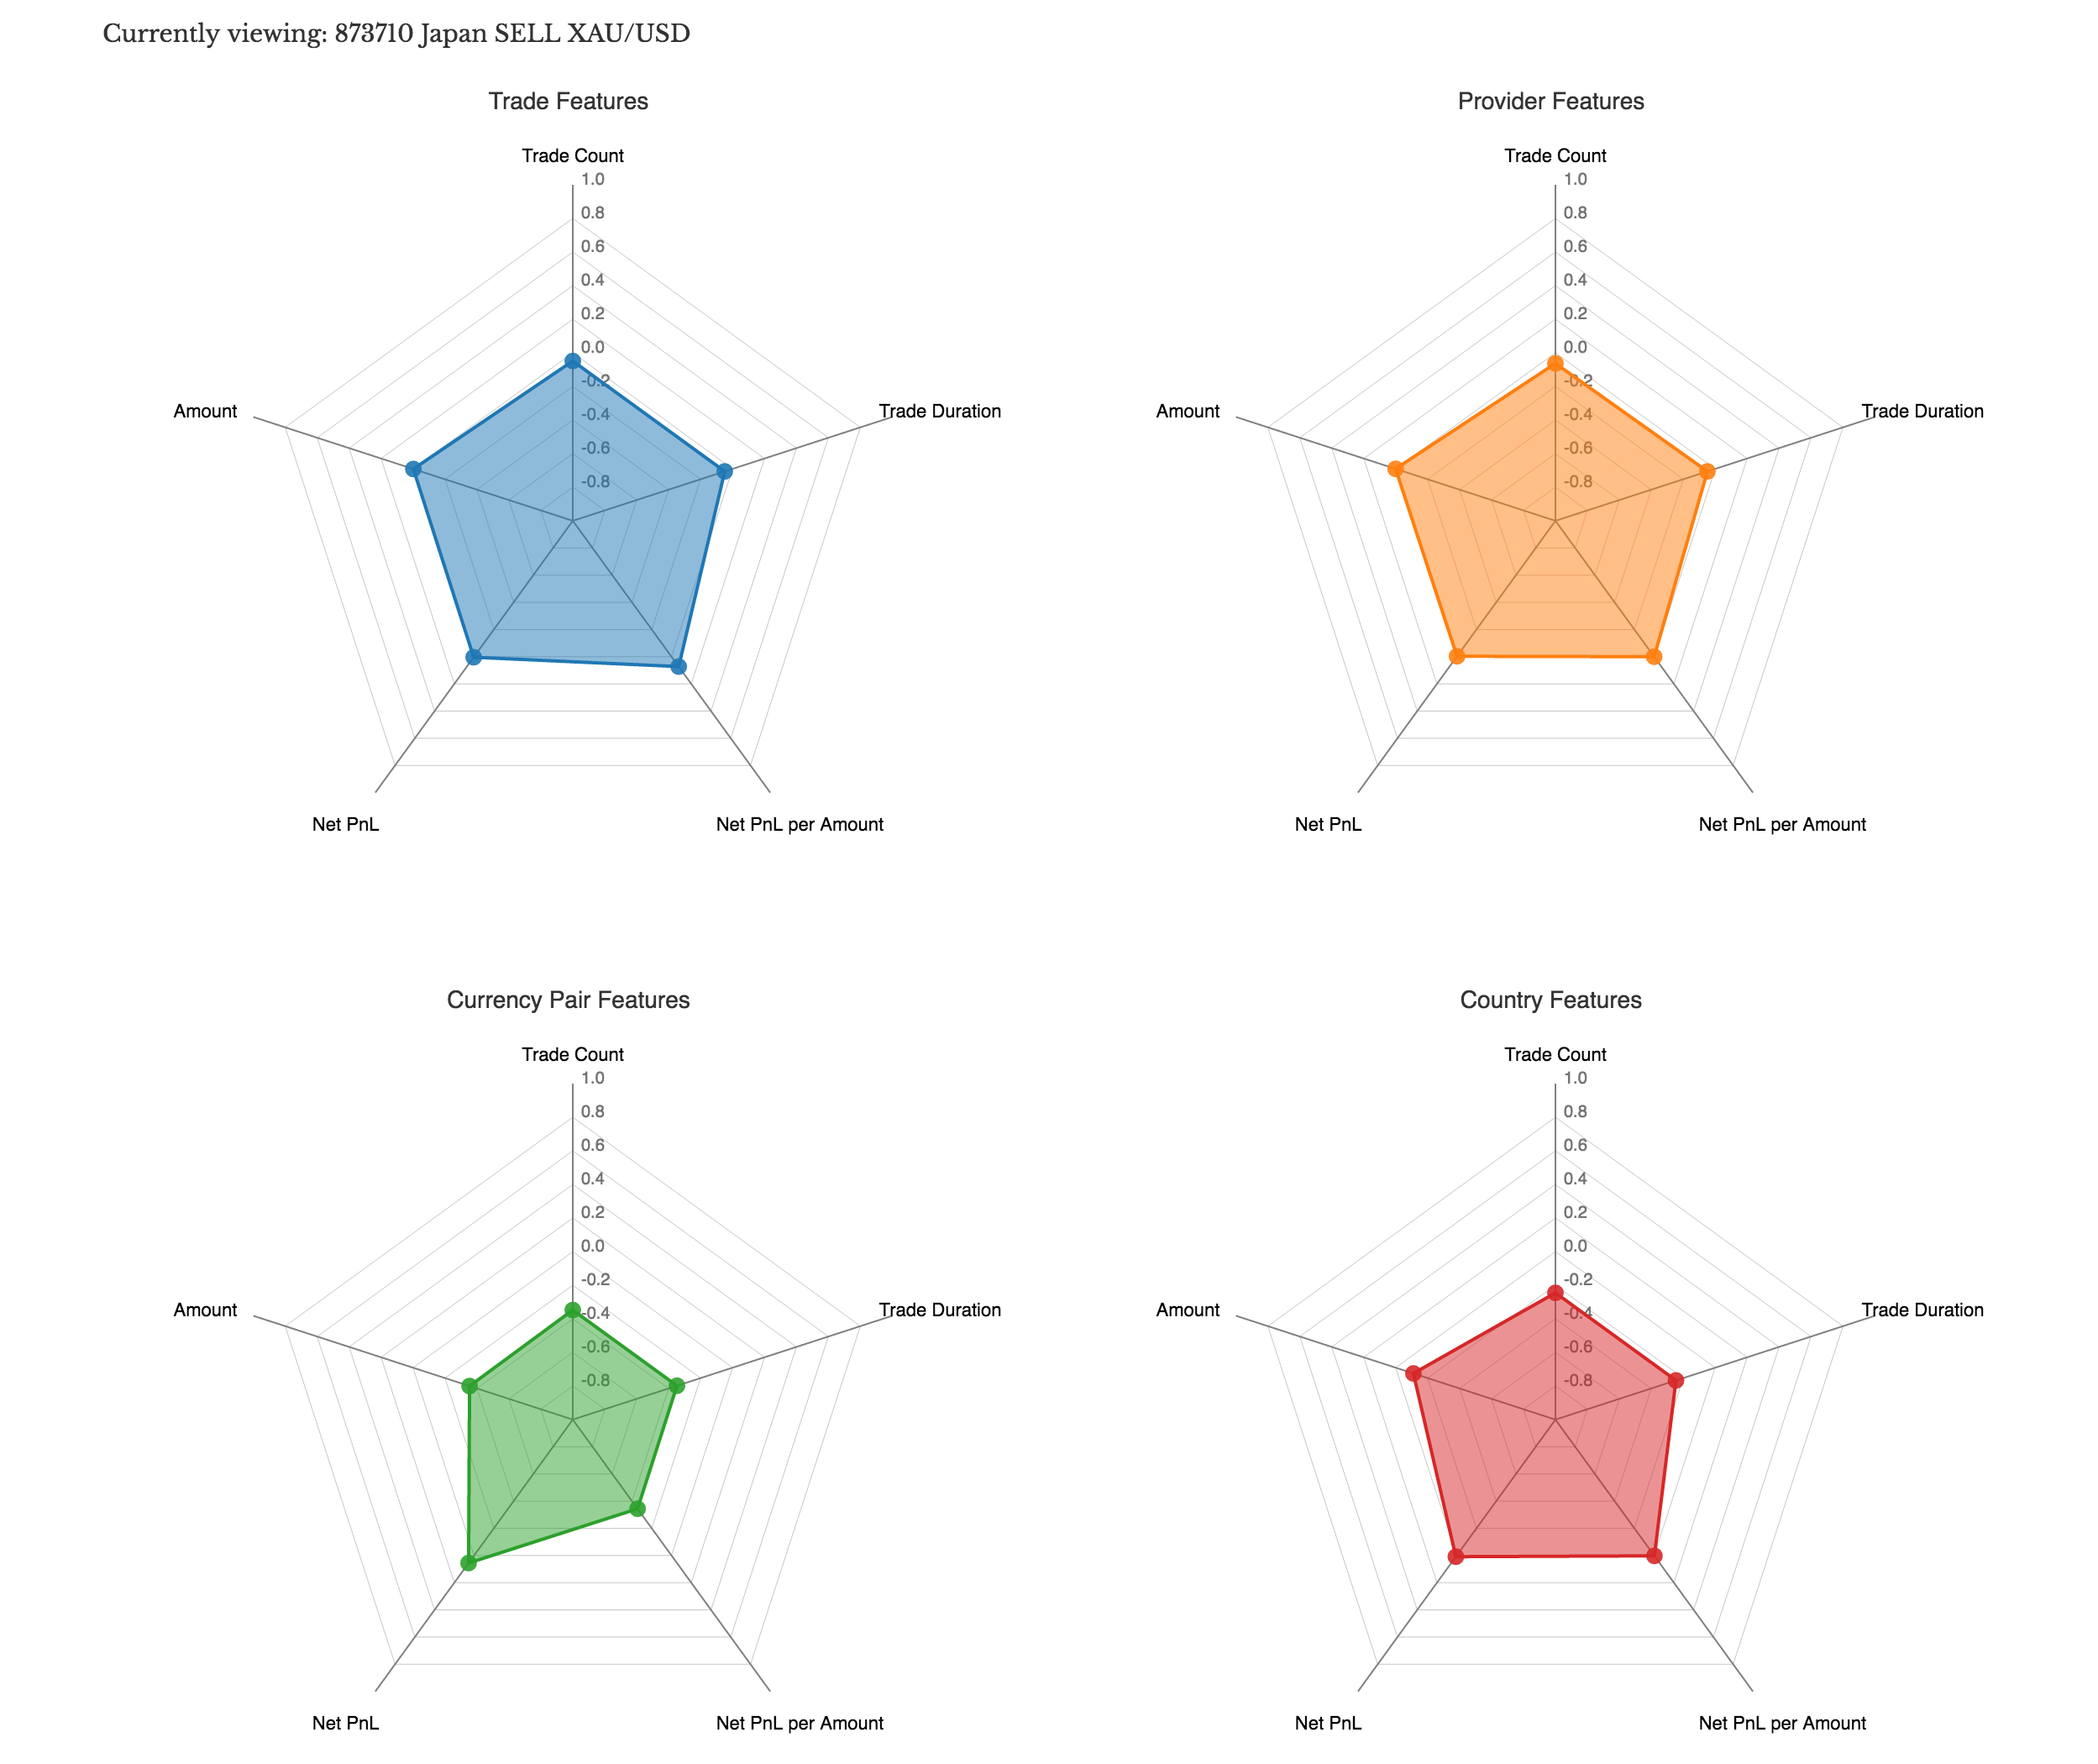
\includegraphics[width=\textwidth]{features_1}
  \label{fig:features_1}
\end{figure}

Παραπάνω βλέπουμε τις κανονικοποιημένες τιμές των χαρακτηριστικών που επιλέξαμε για μια συγκεκριμένη συναλλαγή. Βλέπουμε ότι η συγκεκριμένη συναλλαγή βρίσκεται στον κοντά στο μέσο όρο στα περισσότερα χαρακτηριστικά της, όπως το ίδιο συμβαίνει και με τον συγκεκριμένο χρηματιστή. Από την άλλη βλέπουμε ότι το Ασήμι συναλλάσσεται λίγες φορές (trade count κάτω από τον μέσο όρο) αλλά έχει κέρδη πάνω από τον μέσο όρο. Ενώ για την χώρα, στην περίπτωσή μας η Ιαπωνία, κάνει λιγότερες συναλλαγές από τον μέσο όρο, αλλά και οι συναλλαγές που κάνουν οι χρηματιστές από αυτή τη χώρα έχουν σημαντικά μικρότερη διάρκεια από το μέσο όρο.

Πέρα από τις διαισθήσεις που μπορούμε να αποκτήσουμε πάνω στα δεδομένα μας – ο οποίες μπορούν να χρησιμοποιηθούν σαν ανάδραση για να επιλέξουμε ποια από τα χαρακτηριστικά που διαλέξαμε θα κρατήσουμε ή θα αλλάξουμε – μελετώντας πως συμπεριφέρονται τα οι τιμές των χαρακτηριστικών στις διάφορες συναλλαγές, χρηματιστές, νομίσματα ή χώρες μπορούμε να σκεφτούμε πως θα τις συνδυάσουμε ώστε να βγάλουμε την ψευδο-αξιολόγηση για κάθε συναλλαγή.

Ξανά, στη δικιά μας ανάλυση, επιλέξαμε να μην κρατήσουμε το χαρακτηριστικό Amount, γιατί παρατηρήσαμε ότι είχε μεγάλη διακύμανση ή οποία όμως δεν ήταν σχετική με την ποιότητα της συναλλαγής—γι’ αυτό το λόγο πετάξαμε και το χαρακτηριστικό Net PnL per Amount. 

Αφού επιλέξουμε ποια χαρακτηριστικά θα κρατήσουμε μπορούμε να δούμε πως αυτά συμπεριφέρονται στο σύνολο των συναλλαγών μας. Αφού περάσουμε τις τιμές των χαρακτηριστικών για κάθε συναλλαγή στο Visfx, τρέχουμε το Spark script points.py και εξάγουμε την MDS χωρική απεικόνιση των δεδομένων μας βάση τα επιλεγμένα χαρακτηριστικά. Επίσης μπορούμε να δώσουμε τα βάρη που επιλέξαμε (στη δική μας ανάλυση βγήκαν από τη μέθοδο PCA) και να δούμε με χρώμα πώς κινούνται οι ψευδο-αξιολογήσεις στις συναλλαγές μας. Η κλίμακα είναι από το 0 στο 5 και από το κόκκινο στο μπλε.

\begin{figure}[H]
  \centering
  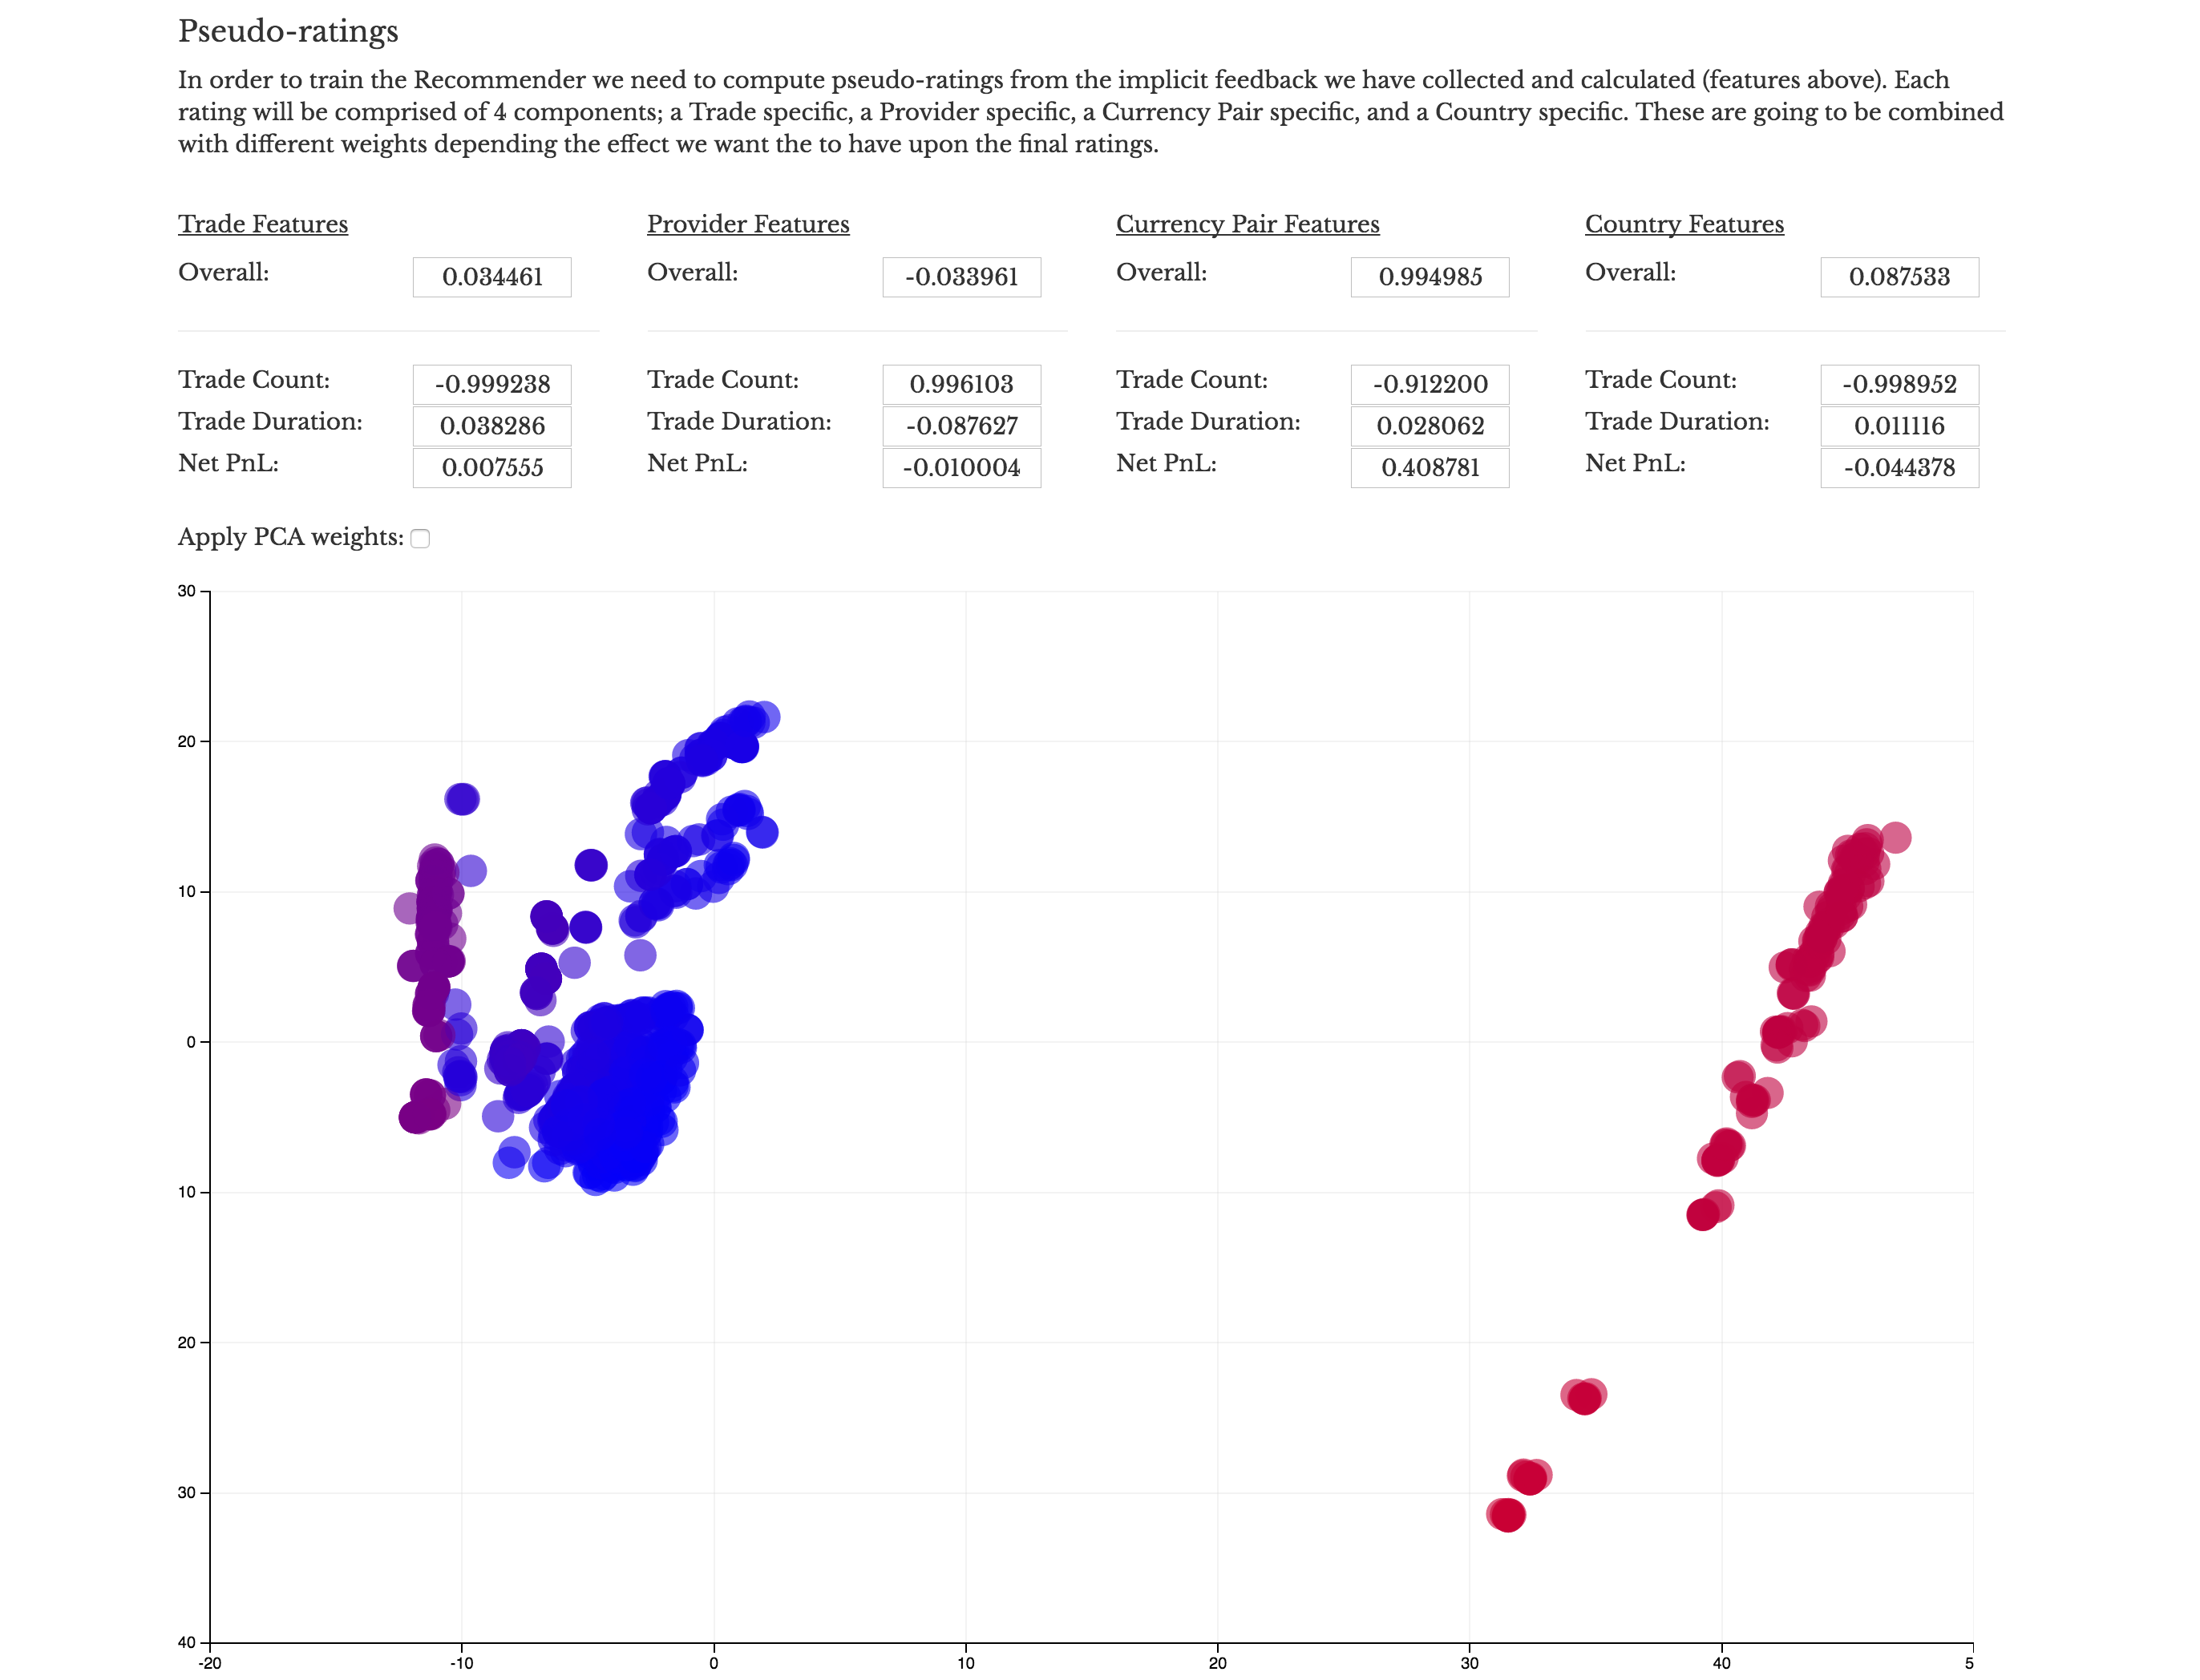
\includegraphics[width=\textwidth]{features_2}
  \label{fig:features_2}
\end{figure}

Εδώ μπορούμε αμέσως να δούμε ότι δημιουργούνται διάφορες ομάδες στις συναλλαγές μας οποίες βαθμολογούνται επίσης διαφορετικά. Έχοντας από τις προηγούμενες απεικονίσεις αποκτήσει γνώση των δεδομένων μας μπορούμε να αξιολογήσουμε αν οι συγκεκριμένες συναλλαγές (που φέρνοντας το ποντίκι πάνω σε κάθε σημείο μπορούμε να δούμε λεπτομέρειες γι’ αυτό) έχουν βαθμολογηθεί σωστά και αμέσως να κάνουμε αλλαγές στον τρόπο υπολογισμού των ψευδο-αξιολογήσεων. Ακόμα αλλάζοντας τις επιλογές στην κορυφή της σελίδα μπορούμε να φιλτράρουμε τα σημεία που εμφανίζονται στο MDS διάγραμμα. 

\begin{figure}[H]
  \centering
  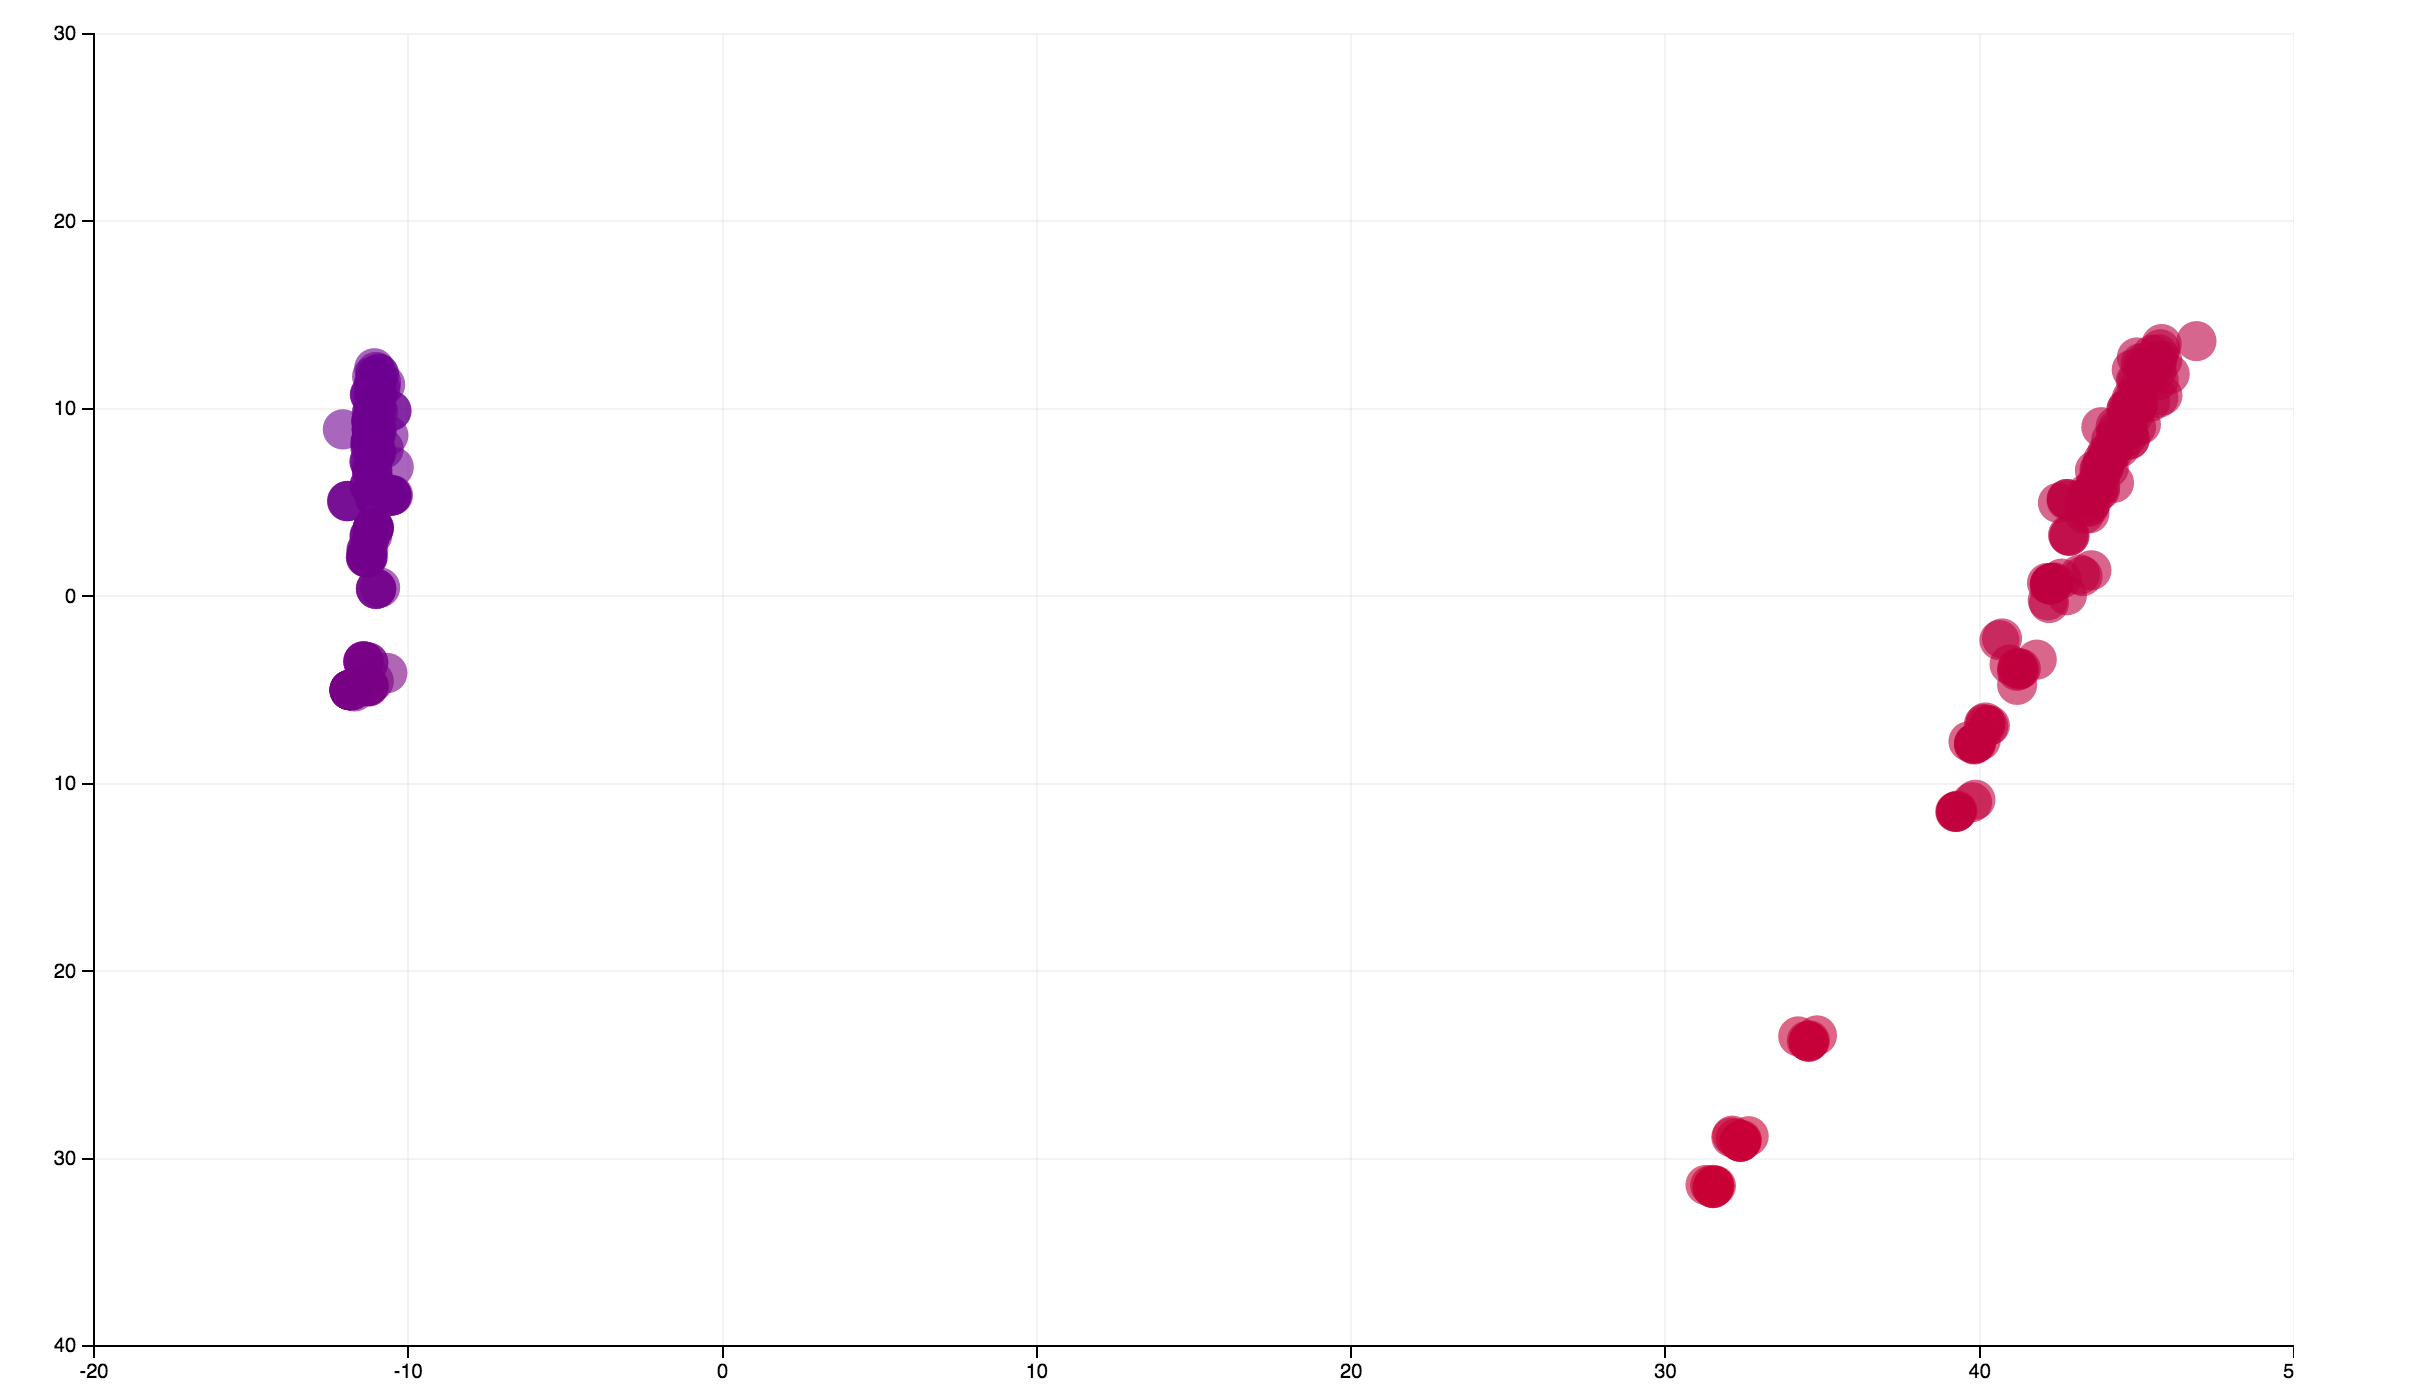
\includegraphics[width=\textwidth]{features_3}
  \label{fig:features_3}
\end{figure}

Παραπάνω φαίνονται οι συναλλαγές που έκαναν χρηματιστές στο ζεύγος EUR/USD και παρακάτω στο GBP/USD

\begin{figure}[H]
  \centering
  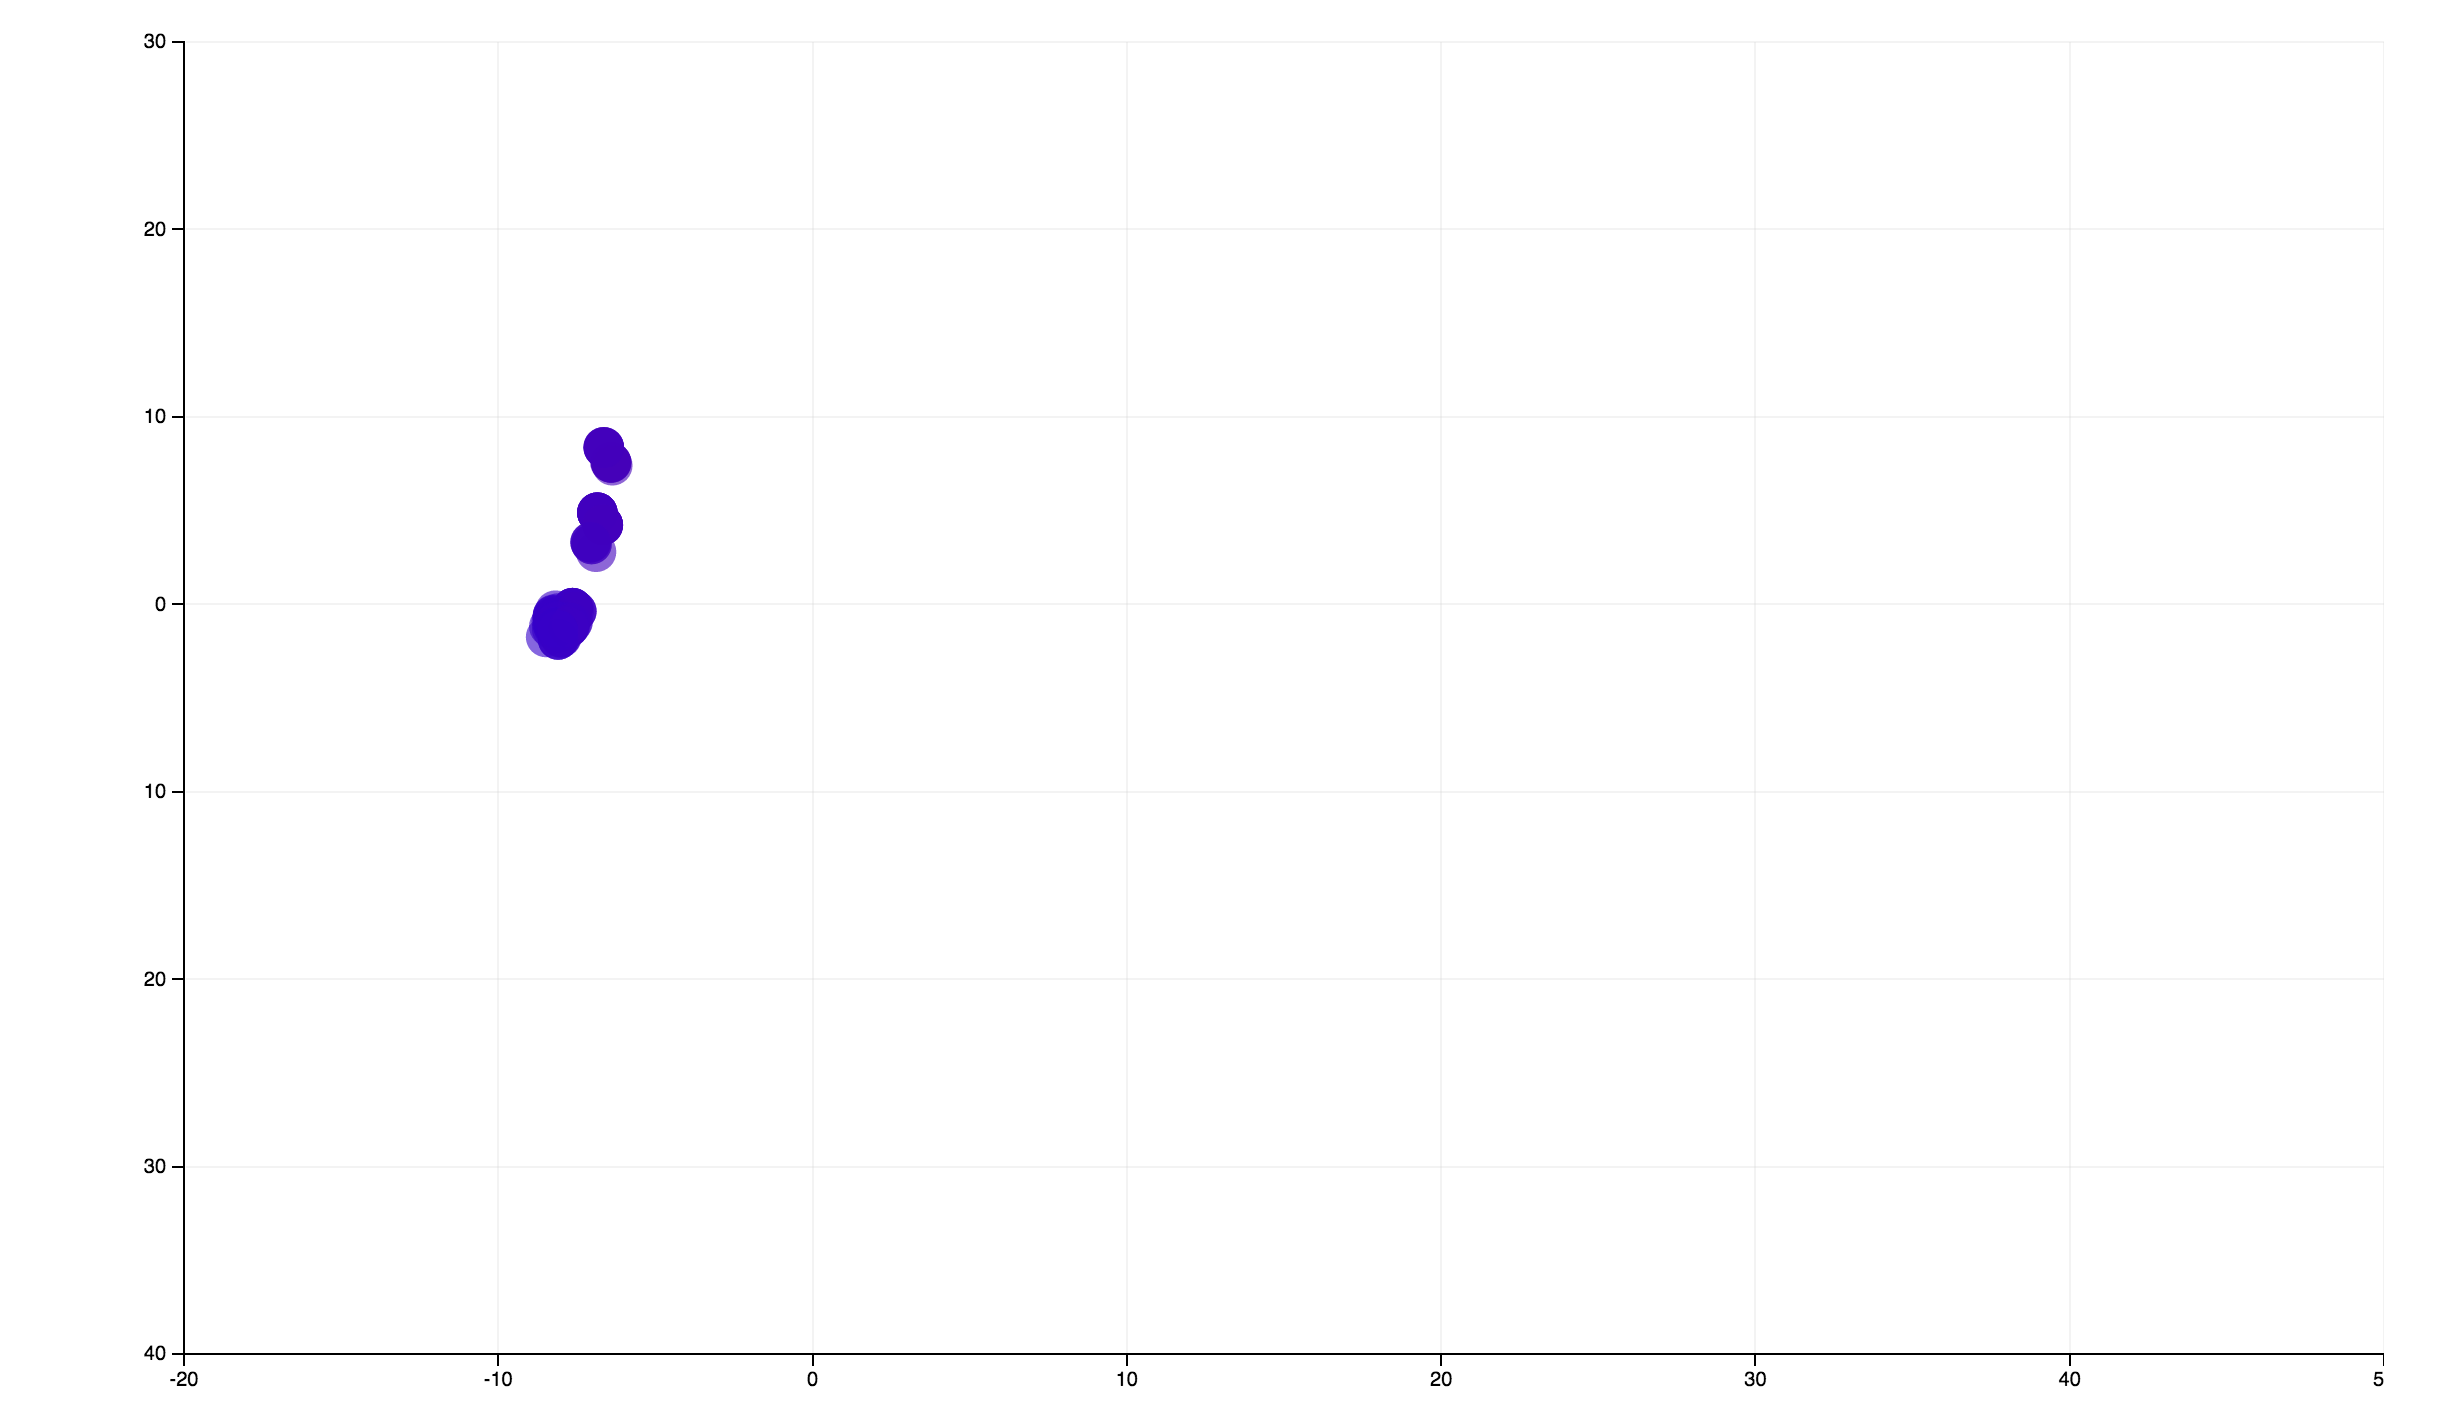
\includegraphics[width=\textwidth]{features_4}
  \label{fig:features_4}
\end{figure}

Παρατηρείται γενικά το φαινόμενο λόγω των ζημιών ότι το EUR/USD βαθμολογείται χαμηλά (κόκκινα και μοβ σημεία) ενώ από την άλλη το GBP/USD βαθμολογείται υψηλά λόγω της δημοφιλίας του και των κερδών του. Έτσι δημιουργείται ένας βρόχος οπτικής ανάδρασης, όπου οι αλλαγές στον τρόπο υπολογισμού των ψευδο-αξιολογήσεων είναι άμεσα εμφανείς και μπορούμε άμεσα να πάρουμε αποφάσεις. Για παράδειγμα αν είχαμε χρησιμοποιήσει διαφορετικά βάρη και αντί το χαρακτηριστικό Net PnL το Net PnL per Amount θα είχαμε τα ακόλουθα αποτελέσματα:

\begin{figure}[H]
  \centering
  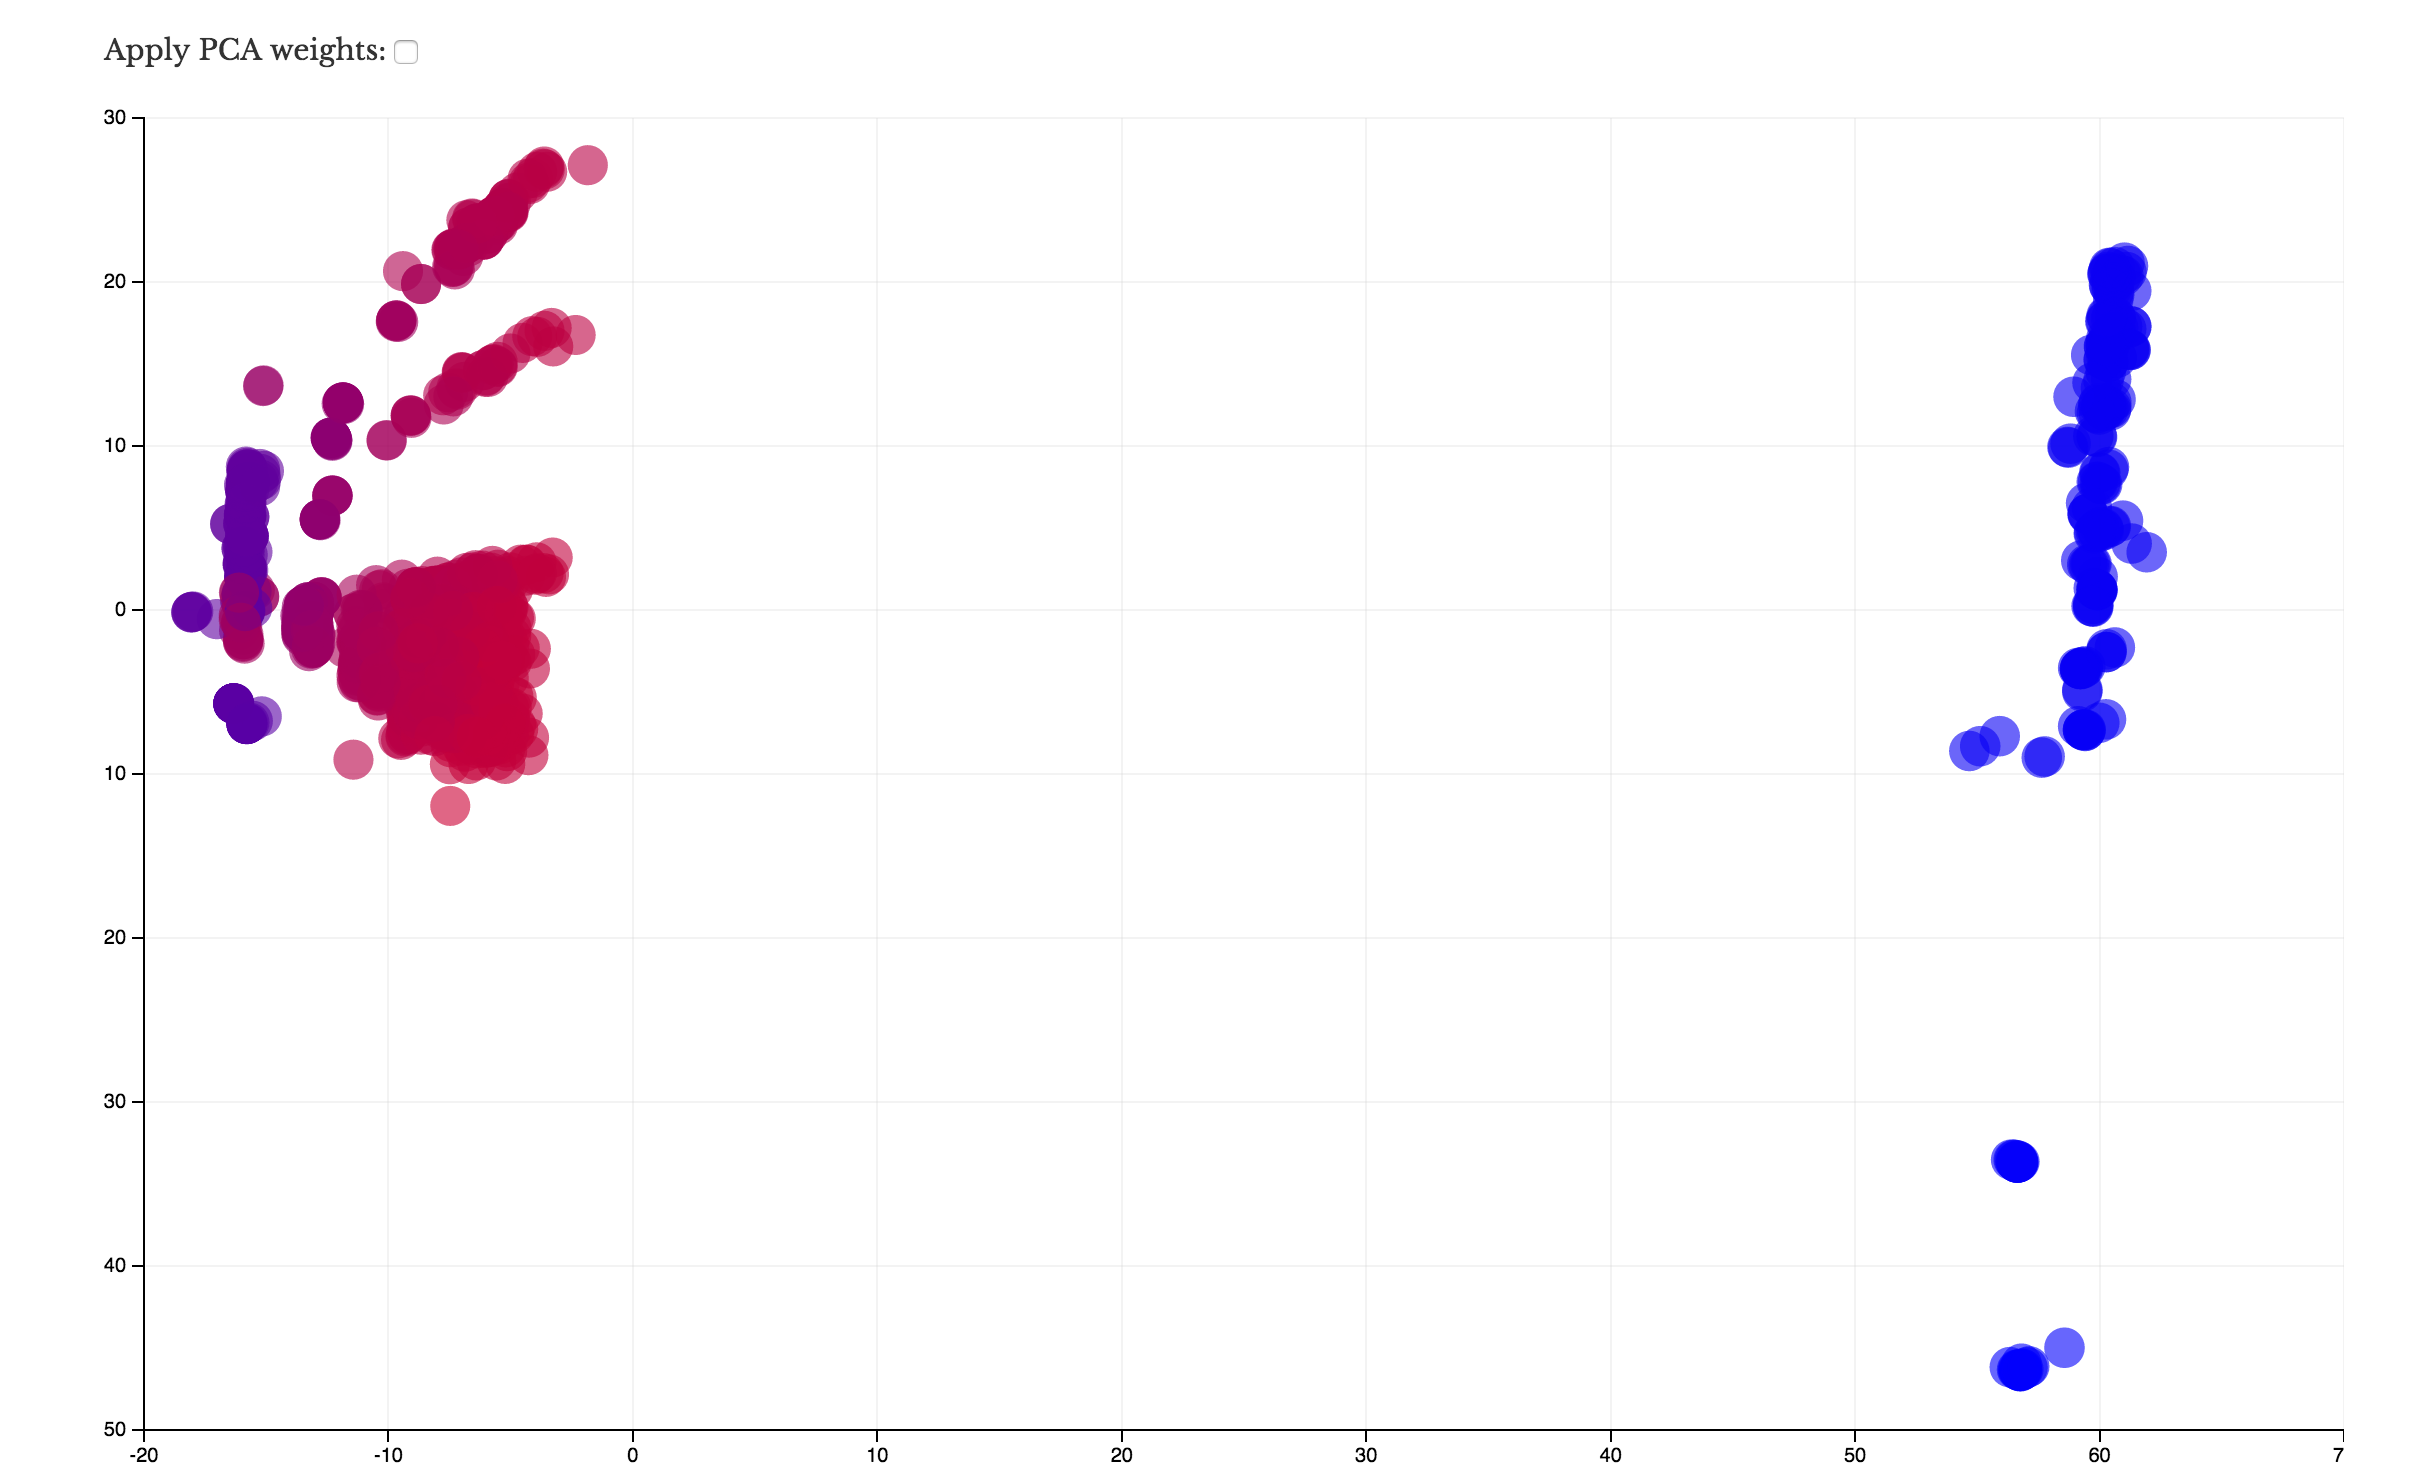
\includegraphics[width=\textwidth]{features_5}
  \label{fig:features_5}
\end{figure}

Αυτό είναι ένα σενάριο το οποίο είχα αρχικά χρησιμοποιήσει αλλά τελικά απορρίψει. Όπως βλέπουμε και στο διάγραμμα, οι συναλλαγές EUR/USD έχουν βαθμολογηθεί υπέρμετρα υψηλότερα από όλες τις υπόλοιπες. Αυτό συνέβη γιατί όπως είδαμε και στην ανάλυση των δεδομένων το ζεύγος αυτό είναι πολύ δημοφιλές, οι χρηματιστές το συναλλάσουν πολλές φορές και βάζουν αντίστοιχα μεγάλα ποσά (amount), αλλά όχι αντίστοιχα κερδοφόρο. Επίσης λόγω της φύσης του αλγορίθμου η δημοφιλία ενός ζεύγους λαμβάνεται ήδη υπόψιν συνεπώς δε θέλουμε να του δώσουμε υπέρμετρα υψηλή αξιολόγηση.

\section{Παρουσίαση Συστάσεων}

Τέλος έχοντας καταλήξει στον τρόπο υπολογισμού των ψευδο-αξιολογήσεων, μπορούμε να τρέξουμε το RS και να αξιολογήσουμε τις επιδόσεις του. Αυτό γίνεται στην τρίτη και τελευταία καρτέλα του Visfx, Recommendations. Εδώ μπορούμε να δούμε μία άμεση επισκόπηση των συστάσεων που δίνουμε στους χρηματιστές μέσω ενός Parallel Coordinates διάγραμμα, όπου με μπλε χρώμα είναι σημειωμένες οι πραγματοποιημένες συναλλαγές και με κόκκινο οι προτάσεις που δώσαμε. 

\begin{figure}[H]
  \centering
  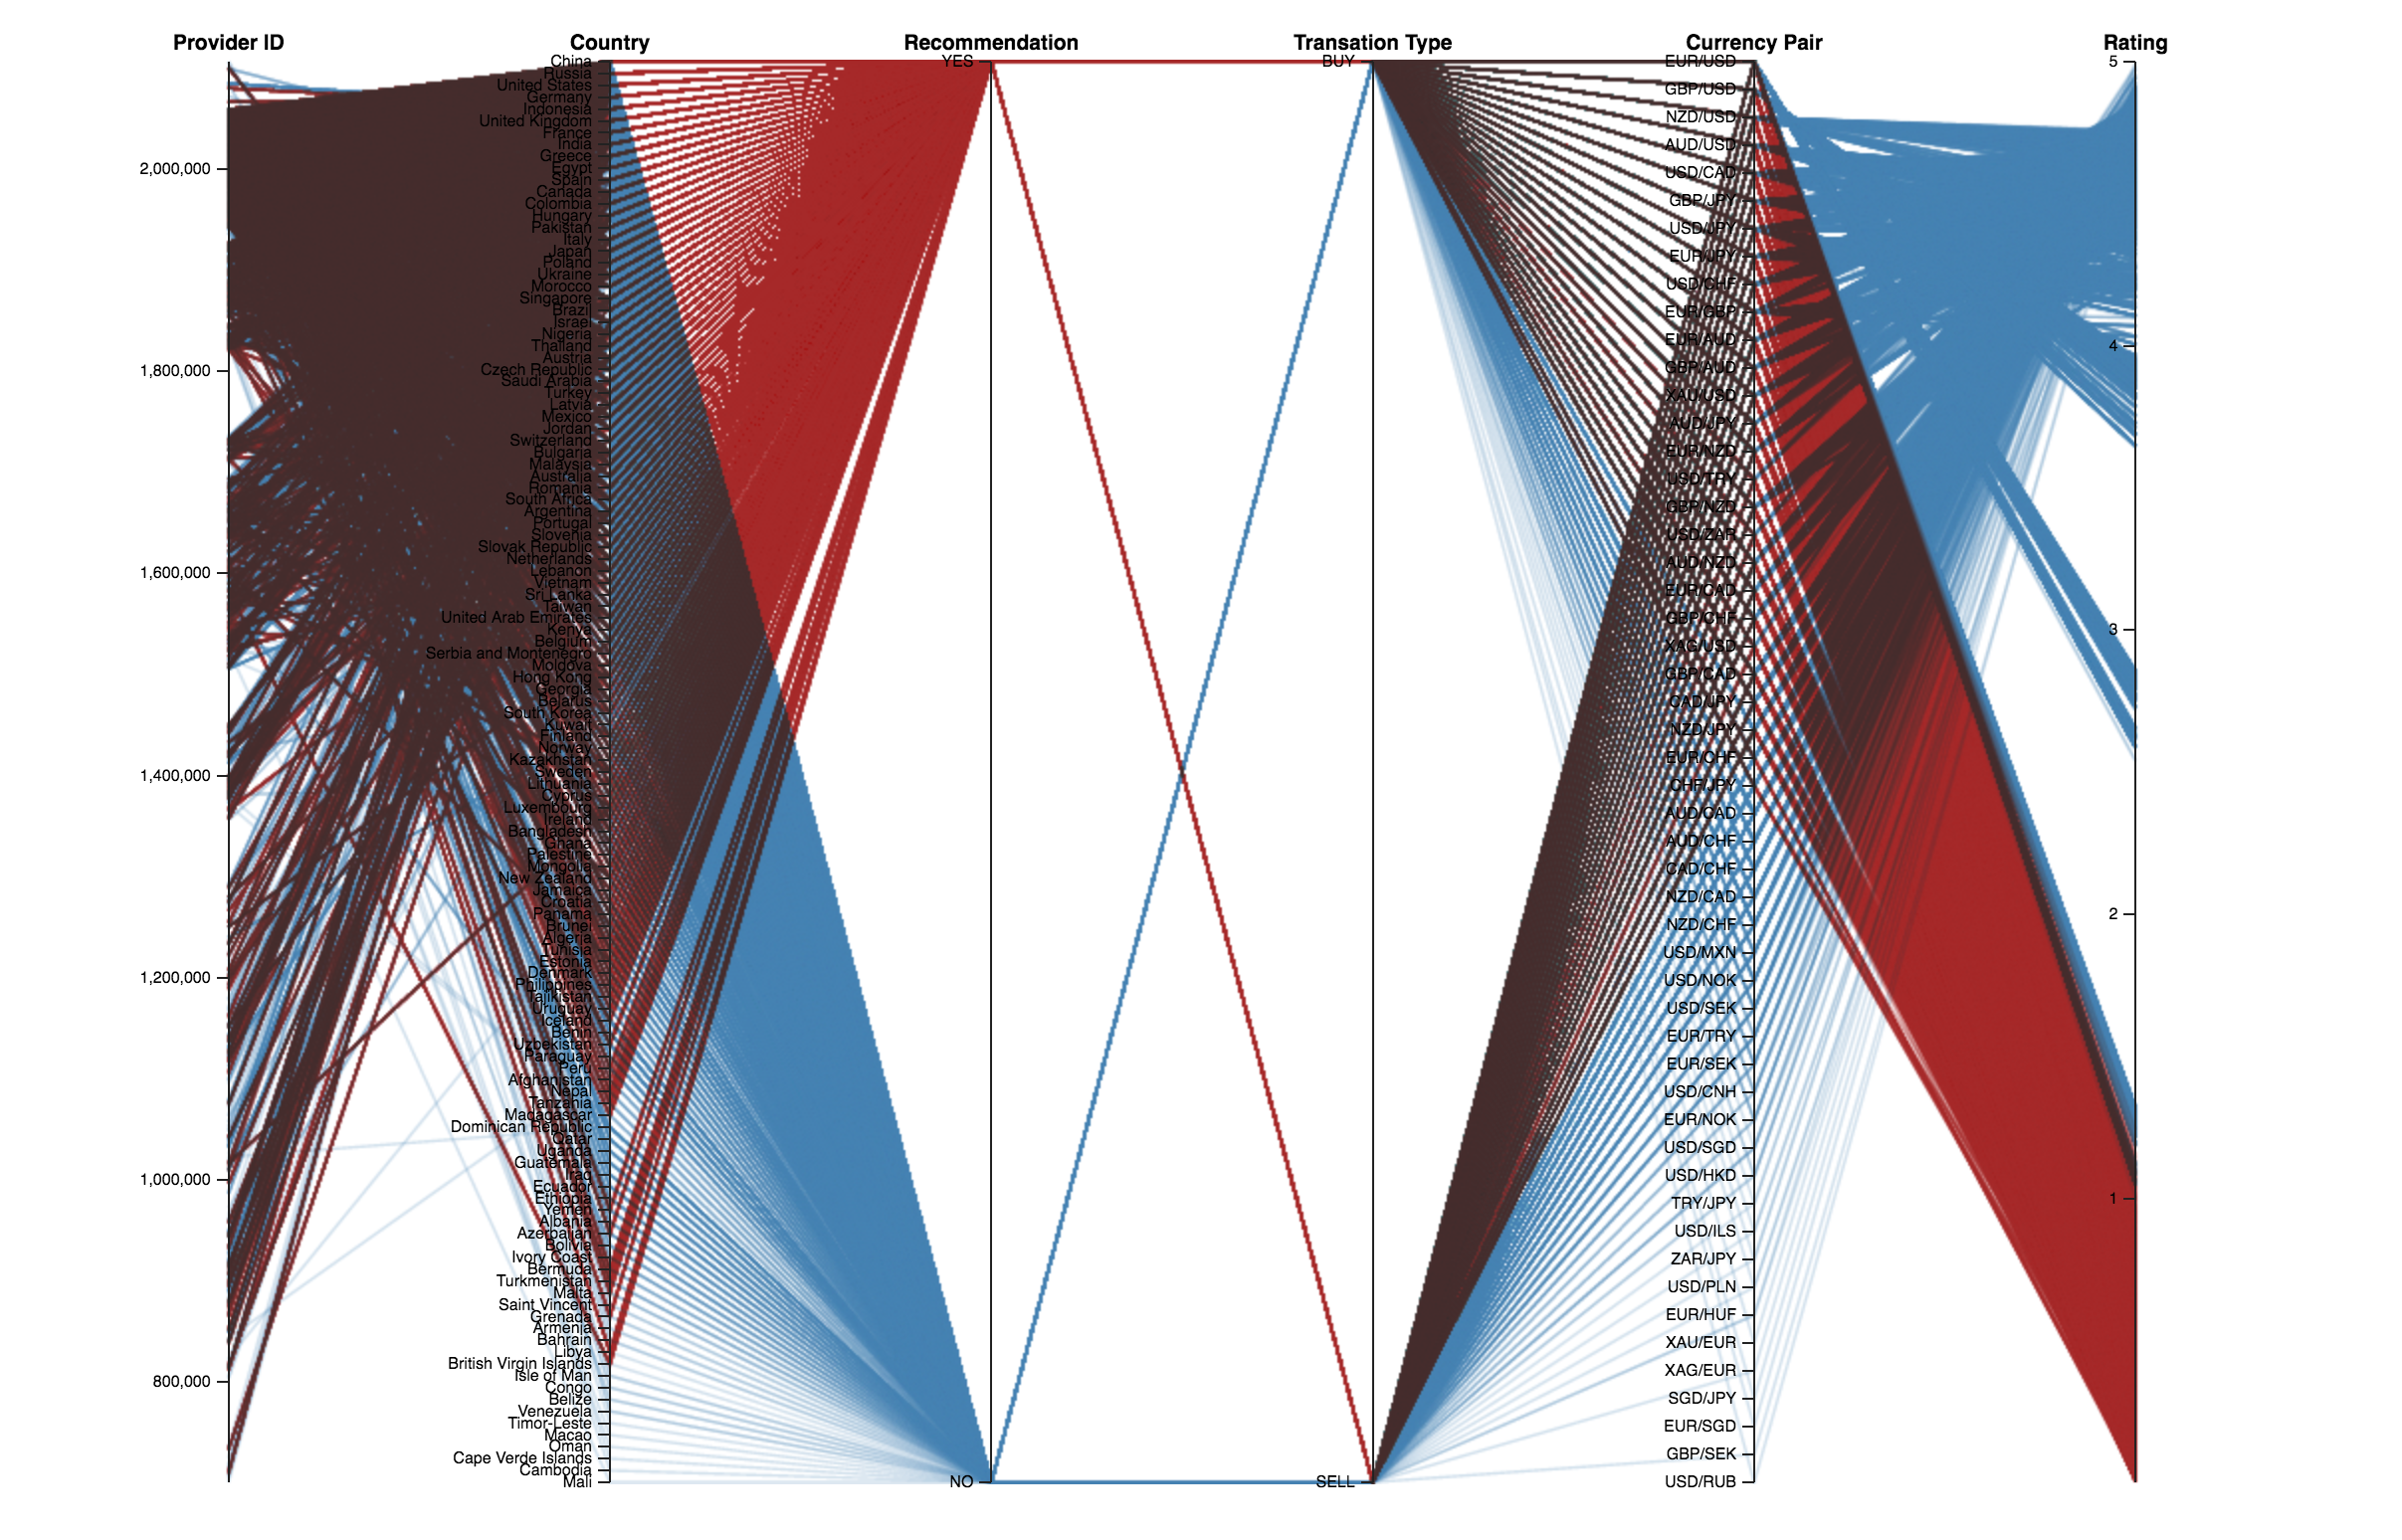
\includegraphics[width=\textwidth]{recommendations_1}
  \label{fig:recommendations_1}
\end{figure}

Στη συνέχεια μπορούμε να επιλέξουμε συγκεκριμένους χρηματιστές και να δούμε τις συναλλαγές που πραγματοποίησαν στο διάστημα το οποίο είχαμε χρησιμοποιήσει για να εκπαιδεύσουμε το RS, τις συναλλαγές που τους προτείναμε για την επόμενη μέρα, αλλά και τι όντως έπραξαν την επόμενη μέρα, ώστε να αξιολογήσουμε την απόδοση του RS.

\begin{figure}[H]
  \centering
  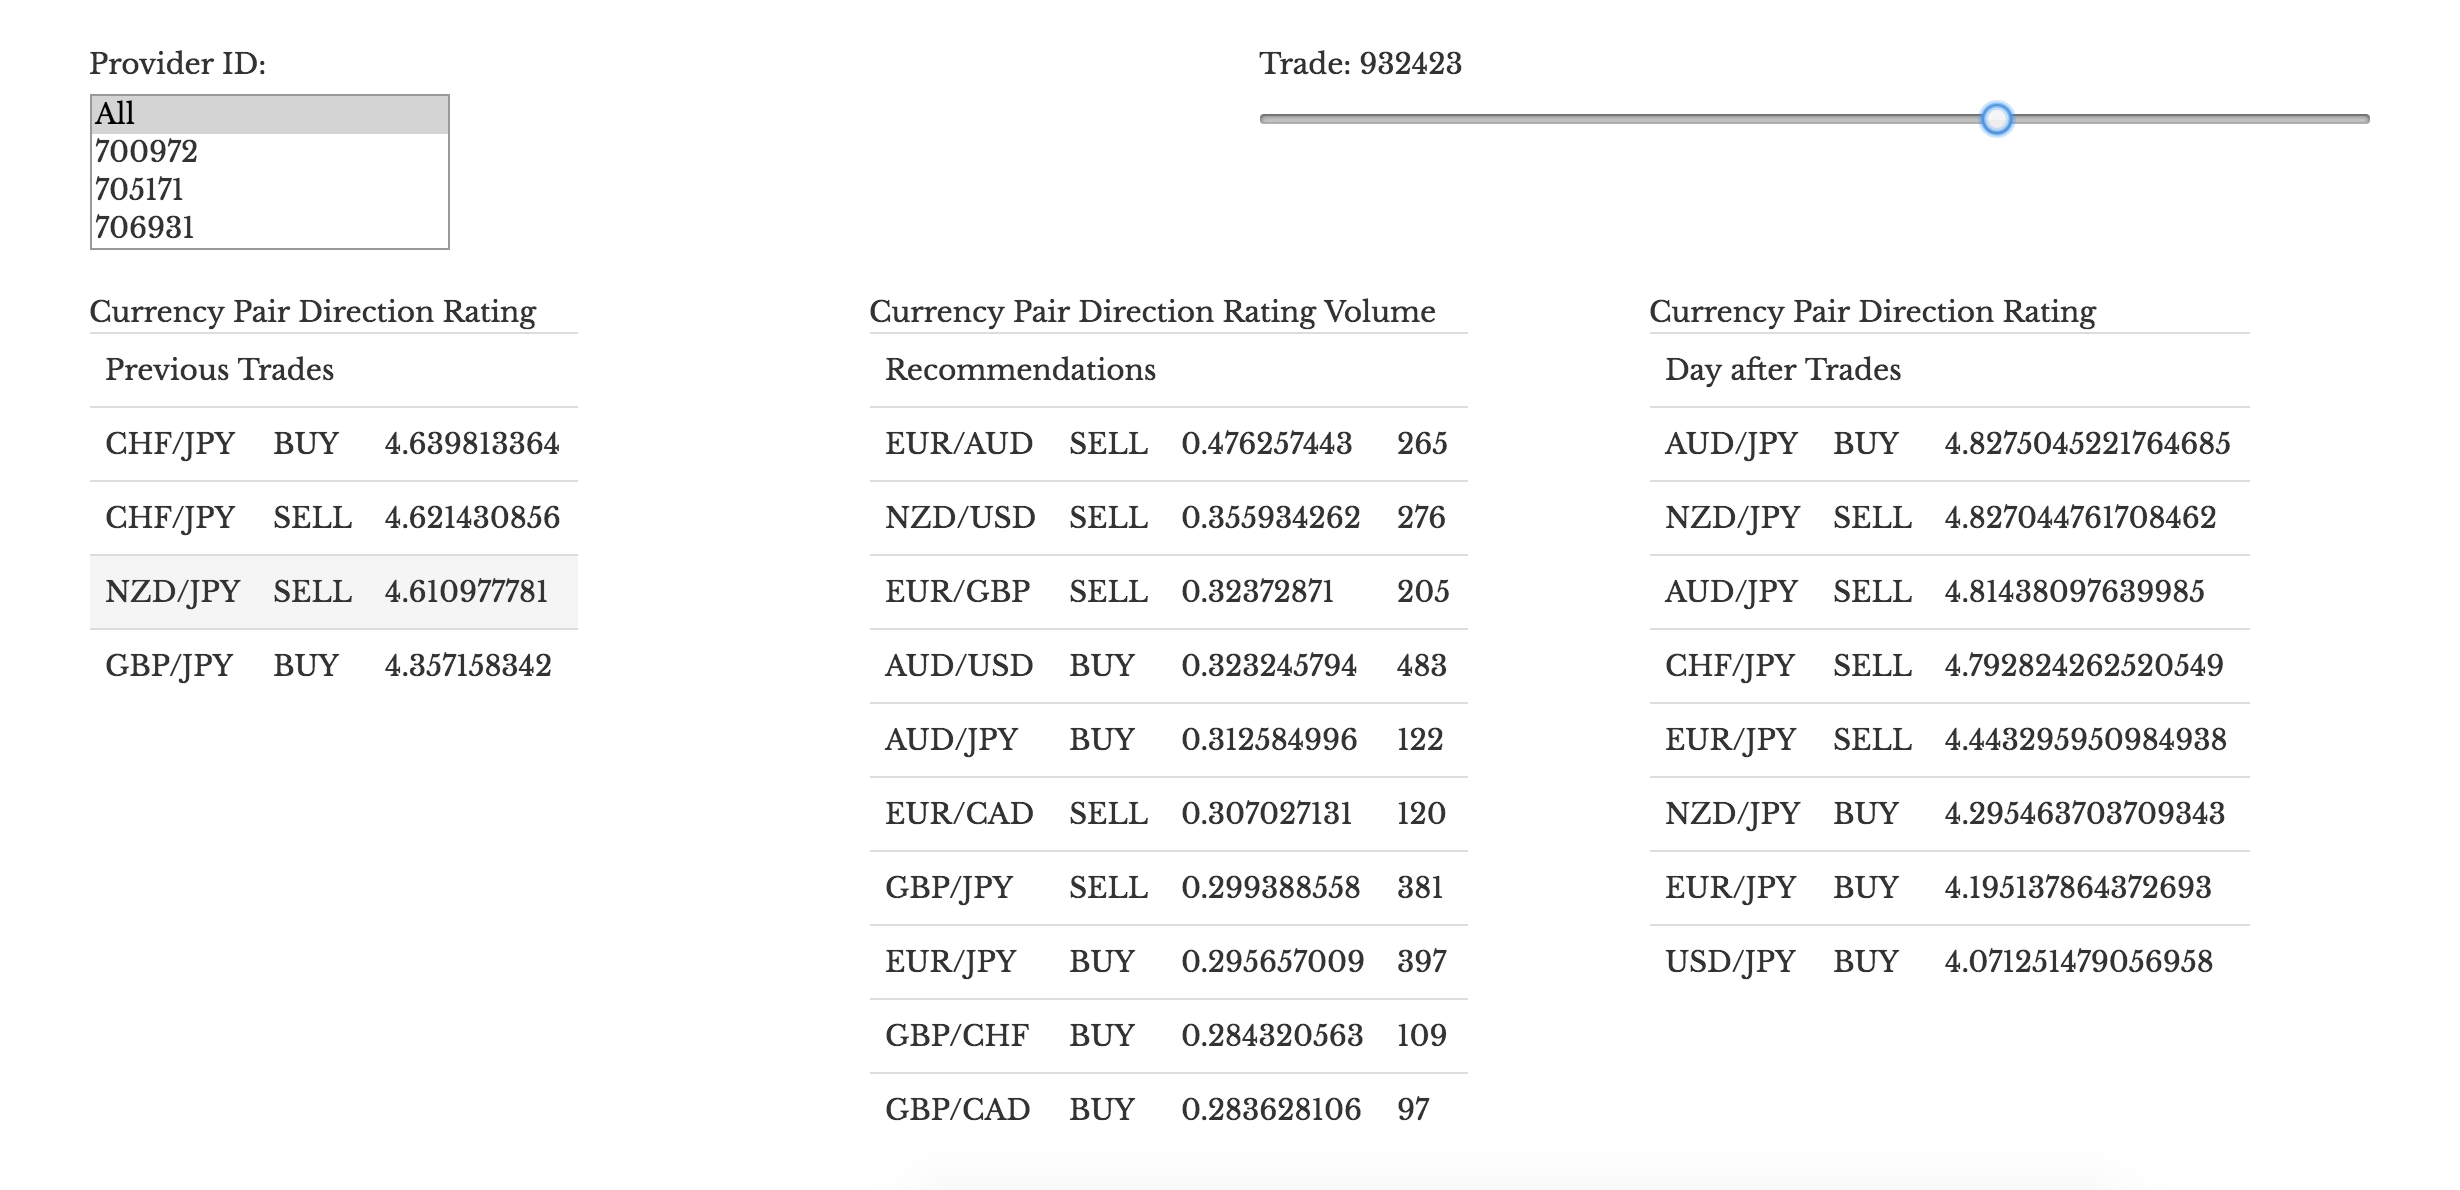
\includegraphics[width=\textwidth]{recommendations_2}
  \label{fig:recommendations_2}
\end{figure}

\begin{figure}[H]
  \centering
  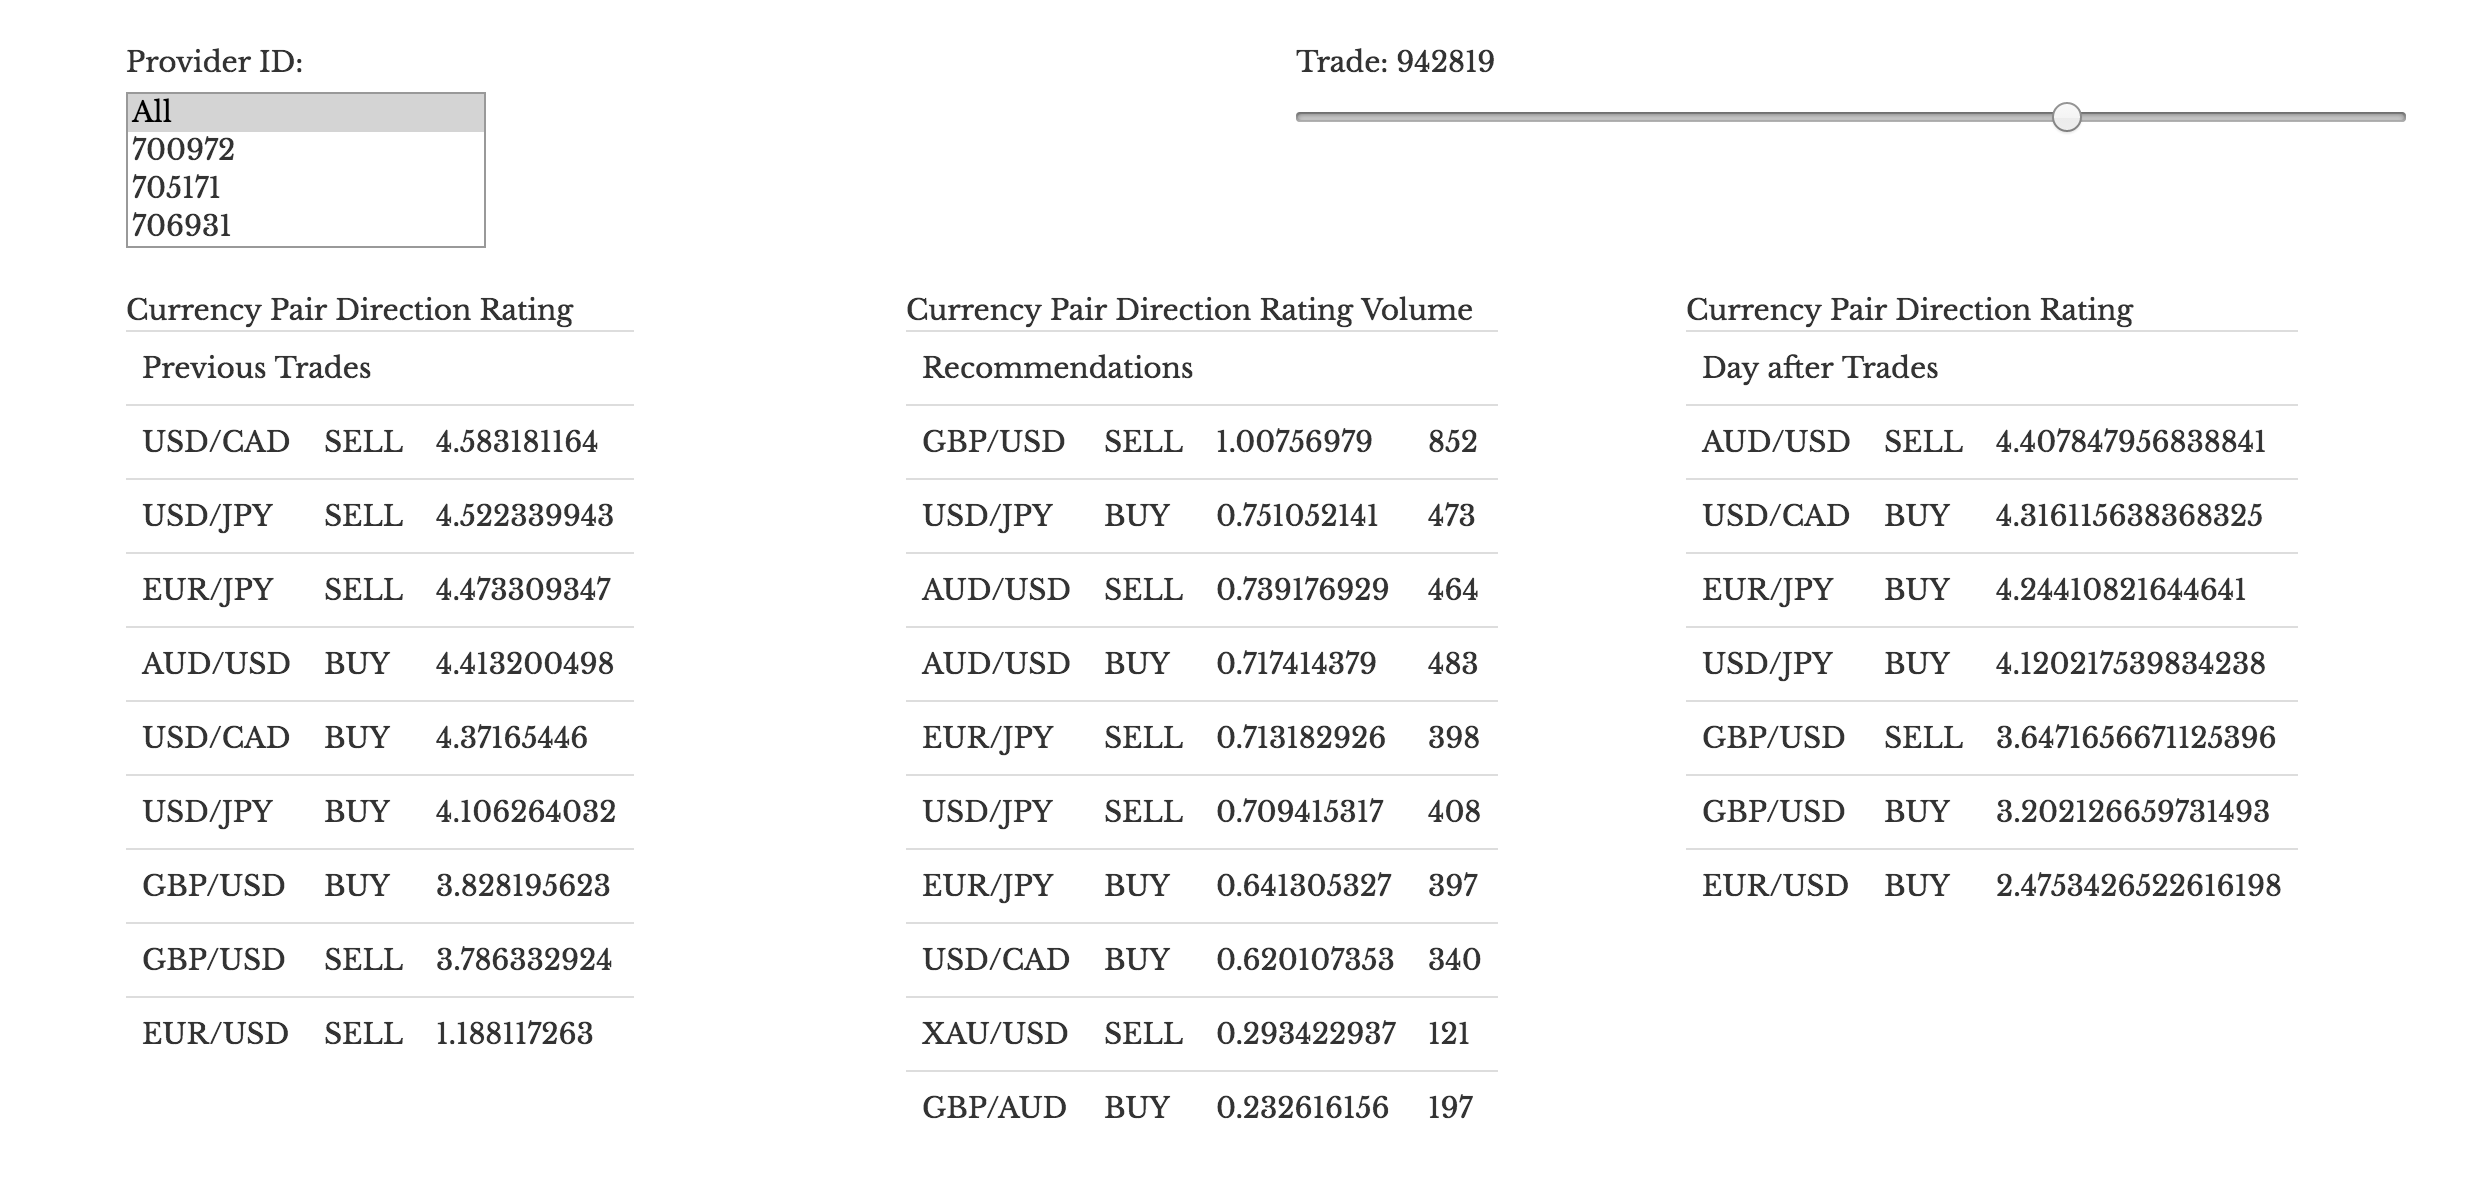
\includegraphics[width=\textwidth]{recommendations_3}
  \label{fig:recommendations_3}
\end{figure}

Όπως βλέπουμε παραπάνω υπάρχει αντιστοιχία στις περισσότερες περιπτώσεις μεταξύ των συστάσεων και των συναλλαγών που πραγματοποίησε ο χρηματιστής την επόμενη εβδομάδα. Αυτό που παρατηρείται σε πολλές περιπτώσεις είναι ότι οι χρηματιστές έχουν ένα σετ από νομισματικά ζεύγη που αγοράζουν ή πουλάνε τακτικά, όμως αυτό δε σημαίνει ότι μία σύσταση πέρα από τα συνηθισμένα ζευγάρια είναι κακή. 

Γι’ αυτό, επίσης παρατίθενται οι τιμές που είχαν πάρει τα νομισματικά ζεύγη που προτείναμε κατά την περίοδο εκπαίδευσης του RS αλλά και τις μέρες που αφορά η παραγόμενη σύσταση ώστε να δούμε αν οι προτάσεις μας θα μπορούσαν να είναι κερδοφόρες σ’ αυτήν την περίοδο, ώστε να αξιολογήσουμε πόσο επικερδής θα ήταν μία συναλλαγή που θα άνοιγε και έκλεινε αυτή την περίοδο. 

\begin{figure}[H]
  \centering
  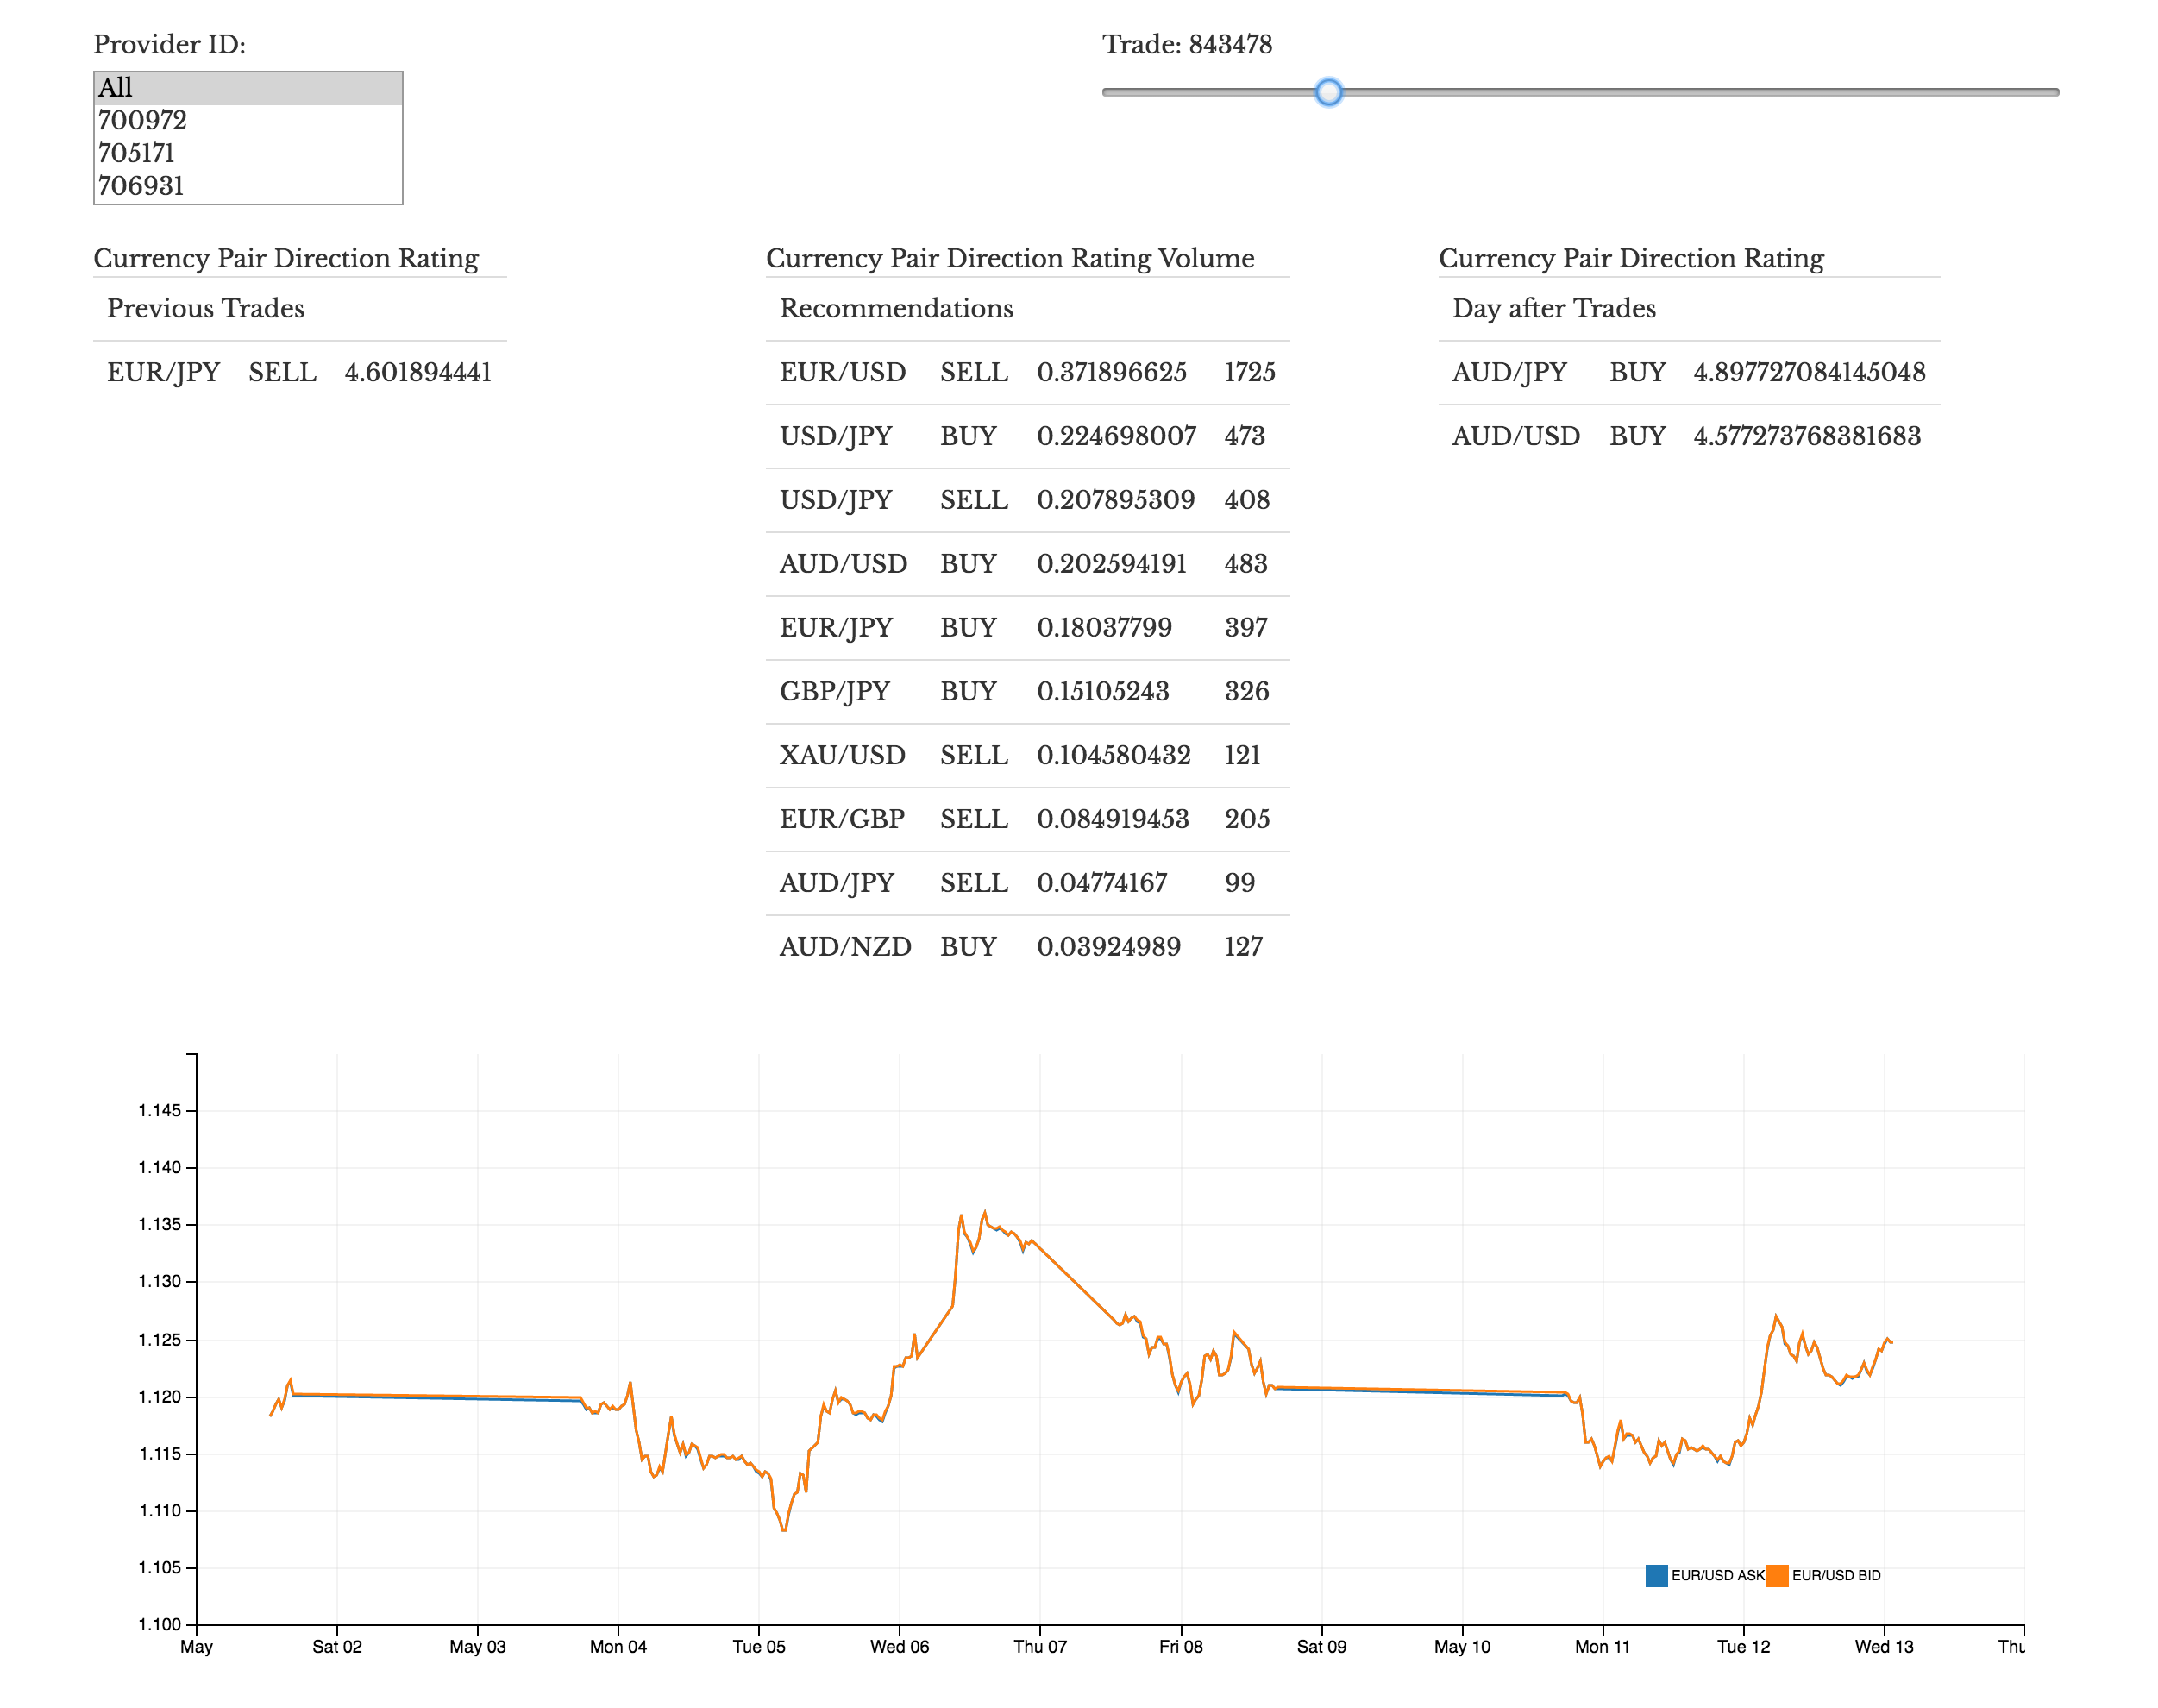
\includegraphics[width=\textwidth]{recommendations_4}
  \label{fig:recommendations_4}
\end{figure}

Όπως βλέπουμε στο παραπάνω γράφημα θα μπορούσε να ανοίξει μία BUY συναλλαγή στο EUR/USD στις 04/05 και να κλείσει στις 07/05 όπου η τιμή αυξήθηκε από 1.118 σε 1.133.

Μ’ αυτόν τον τρόπο μπορούμε να αξιολογήσουμε την ποιότητα του RS συγκρίνοντας τις συστάσεις μας με το τι πραγματικά έκανε ο χρηματιστής, και να δούμε αν χρειάζεται να μεταβάλουμε τα χαρακτηριστικά του RS ώστε να δίνει καλύτερες συστάσεις.

\clearemptydoublepage

\chapter{Συμπεράσματα}\label{ch:chap4}
\input{chapters/chapter_7.tex}
\clearemptydoublepage

%!TEX root = ./main.tex

\begin{thebibliography}{99}

\bibitem{c1} S. C. Park, M. K. Park, and M. G. Kang, “Super-resolution image reconstruction:
A technical overview,” IEEE Signal Processing Magazine, vol. 20, no. 3, pp. 21–36,
May 2003.
\bibitem{keren} D. Keren, S. Peleg, and R. Brada, “Image sequence enhancement using subpixel
displacements,” in IEEE Computer Society Conference on Computer Vision and
Pattern Recognition, June 1988, pp. 742–746.
\bibitem{hardie} R. Hardie, K. Barnard, and E. Armstrong, “Joint MAP registration and high resolution image estimation using a sequence of undersampled images,” IEEE Transactions on Image Processing, vol. 6, no. 12, pp. 1621–1633, December 1997.
\bibitem{patti} A. Patti, M. Sezan, and A. Tekalp, “High-resolution image reconstruction from
a low-resolution image sequence in the presence of time-varying motion blur,” in
Proceedings of the IEEE International Conference on Image Processing, Austin,
TX, vol. 1, 1994, pp. 343–347.
\bibitem{hardie2} R. C. Hardie, K. J. Barnard, J. G. Bognar, E. E. Armstrong, and E. A. Watson, “High resolution image reconstruction from a sequence of rotated and translated
frames and its application to an infrared imaging system,” Optical Engineering,
vol. 37, no. 1, pp. 247–260, January 1998.
\bibitem{alam} M. S. Alam, J. G. Bognar, R. C. Hardie, and B. J. Yasuda, “Infrared image registration and high-resolution reconstruction using multiple translationally shifted aliased video frames,” IEEE Transactions on Instrumentation and Measurement, vol. 49,
no. 5, pp. 923–915, October 2000.
\bibitem{tsai} R. Y. Tsai and T. S. Huang, “Multiframe image restoration and registration,” in Advances in Computer Vision and Image Processing: Image Reconstruction from Incomplete Observations, T. S. Huang, Ed., vol. 1. London: JAI Press, 1984, pp. 317–339.
\bibitem{kim} N. K. Bose, H. C. Kim, and H. M. Valenzuela, “Recursive total least squares algorithm for image reconstruction from noisy undersampled frames,” Multidimensional Systems and Signal Processing, vol. 4, no. 3, pp. 253–268, July 1993.
\bibitem{yang} J. Yang, J. Wright, T. Huang, and Yi Ma. Image super-resolution via sparse representation. IEEE Transactions on Image Processing (TIP), vol. 19, issue 11, 2010.
\bibitem{ransac} Martin A. Fischler and Robert C. Bolles (June 1981). “Random Sample Consensus: A Paradigm for Model Fitting with Applications to Image Analysis and Automated Cartography”. Comm. of the ACM 24 (6): 381–395
\bibitem{wired_ff_algo} Jordan Ellenberg, ”Fill in the Blanks: Using Math to Turn Lo-Res Datasets Into Hi-Res Samples”, 22 February 2010, Wired Magazine \url{http://www.wired.com/2010/02/ff_algorithm/}
\bibitem{incoherence} D.L. Donoho and X. Huo, “Uncertainty principles and ideal atomic decomposition,” IEEE Trans. Inform. Theory, vol. 47, no. 7, pp. 2845–2862, Nov. 2001.
\bibitem{candes} E. Candes, “Compressive sensing,” in Proceedings of the International Congress of Mathematicians, vol. 3, pp. 1433–1452, 2006.
\bibitem{donoho} D. L. Donoho, “Compressed sensing,” IEEE Transactions on Information Theory, vol. 52, no. 4, pp. 1289–1306, 2006.
\bibitem{proakis_sampling} John G. Proakis, Dimitris G. Manolakis , “Digital Signal Processing - Principles, Algorithms, Implementations” 4th edition (Pearson International Edition), Pearson Education, Chapter 1.4.2: The Sampling Theorem 
\bibitem{gonzalez_2d_fft} Rafael C. Gonzalez, Richard E. Woods , “Digital Image Processing” 3rd edition (Pearson International Edition), Pearson Education, Chapter 1.4.2: The 2D Discrete Fourier Transform and its Inverse
\bibitem{shift_add_fusion} S. Farsiu, M. Elad, P. Milanfar, “Fast and Robust Multiframe Super Resolution” IEEE Transactions on Image Processing, vol. 13, no. 10, October 2004
\bibitem{imregintro} ”Image Registration", in Wikipedia: The Free Encyclopedia; (Wikimedia Foundation Inc., updated 2 December 2014, 15:50 UTC) \url{http://en.wikipedia.org/wiki/Image_registration}
\bibitem{cs_intro} M. Davenport, M. Duarte, Y. Eldar, G. Kutyniok, ”Introduction to Compressed Sensing”, Stanford University - Department of Statistics
\bibitem{convexmin} F. Bach, R. Jenatton, J. Mairal, G. Obozinski, ”Convex Optimization with Sparsity-Inducing Norms”, Institut National de Recherche en Informatique et en Automatique (INRIA)
\bibitem{red_dict} H. Rauhut, K. Schnass, and P. Vandergheynst, “Compressed sensing and redundant dictionaries,” IEEE Transactions on Information Theory, vol. 54, no. 5, May 2008.
\bibitem{denoising_dict} M. Elad and M. Aharon, “Image denoising via sparse and redundant representations over learned dictionaries,” IEEE Transactions on Image Processing, vol. 15, pp. 3736–3745, 2006.
\bibitem{im_vid_rest} J. Mairal, G. Sapiro, and M. Elad, “Learning multiscale sparse representations for image and video restoration,” Multiscale Modeling and Simulation, vol. 7, pp. 214–241, 2008.
\bibitem{ksvd_dict} M. Aharon, M. Elad, and A. Bruckstein, “K-SVD: An algorithm for designing overcomplete dictionaries for sparse representation,” IEEE Transactions on Signal Processing, vol. 54, no. 11, pp. 4311–4322, Nov. 2006.
\bibitem{sparse_coding_dict} H. Lee, A. Battle, R. Raina, and A. Y. Ng, “Efficient sparse coding algorithms,” in Advances in Neural Information Processing Systems (NIPS), pp. 801–808, 2007.
\bibitem{human_sparse} B. Olshausen and D. Field, “Sparse coding with an overcomplete basis set: A strategy employed by V1?,” Vision Research, vol. 37, no. 23, pp. 3311–3325, 1997.
\bibitem{nphard} ”NP-hard", in Wikipedia: The Free Encyclopedia; (Wikimedia Foundation Inc., updated 9 April 2015, 15:30 UTC) \url{http://en.wikipedia.org/wiki/NP-hard}
\bibitem{nphard1} D. L. Donoho, “For most large underdetermined systems of linear equations, the minimal $l_1$-norm solution is also the sparsest solution,” Communications on Pure and Applied Mathematics, vol. 59, no. 6, pp. 797–829, 2006.
\bibitem{nphard2} “For most large underdetermined systems of linear equations, the minimal $l_1$-norm near-solution approximates the sparsest near-solution,” Communications on Pure and Applied Mathematics, vol. 59, no. 7, pp. 907–934, 2006.
\bibitem{lasso} R. Tibshirani, “Regression shrinkage and selection via the lasso,” Jour- nal of Royal Statistical Society, Series B, vol. 58, no. 1, 1996.
\bibitem{dict_training} Jianchao Yang, Zhaowen Wang, Zhe Lin, and Thomas Huang. Coupled dictionary training for image super-resolution. IEEE Transactions on Image Processing (TIP), vol. 21, issue 8, pages 3467-3478, 2012.
\bibitem{srexample} W. T. Freeman, T. R. Jones, and E. C. Pasztor, “Example-based superresolution,” IEEE Computer Graphics and Applications, vol. 22, pp. 56–65, 2002.
\bibitem{lowlevel} W. T. Freeman, E. C. Pasztor, and O. T. Carmichael, “Learning low-level vision,” International Journal of Computer Vision, vol. 40, no. 1, pp. 25–47, 2000.
\bibitem{sr_neigh} H. Chang, D.-Y. Yeung, and Y. Xiong, “Super-resolution through neighbor embedding,” in IEEE Conference on Computer Vision and Pattern Classifi- cation (CVPR), vol. 1, pp. 275–282, 2004.
\bibitem{imhal} J. Sun, N. N. Zheng, H. Tao, and H. Shum, “Image hallucination with primal sketch priors,” in IEEE Conference on Computer Vision and Pattern Recognition (CVPR), vol. 2, 2003, pp. 729–736.
\bibitem{imfill} imfill, Image Processing Toolbox Documentation, MathWorks \\ \url{http://www.mathworks.com/help/images/ref/imfill.html}
\bibitem{imresize} imresize, Image Processing Toolbox Documentation, MathWorks \\ \url{http://www.mathworks.com/help/images/ref/imresize.html}
\bibitem{k-term} A. Cohen, W. Dahmen, R. DeVorce, "Compressed sensing and best k-term approximation", in the Journal of the American Mathematical Society, vol. 22, pp. 211-231 , 2009.




\end{thebibliography}

\clearemptydoublepage

\pagestyle{empty}

\vspace*{\fill}
\hline
\begin{flushleft}
	Πανεπιστήμιο Πατρών, Πολυτεχνική Σχολή \\
	Τμήμα Ηλεκτρολόγων Μηχανικών και Τεχνολογίας Υπολογιστών \\
	\me \\
	© \monthyear \ -- Με την επιφύλαξη παντός δικαιώματος.\\
\end{flushleft}
\hline


\end{document}
